\documentclass[tikz,crop,convert={density=200,outext=.png},border=0.4cm]{standalone}

\usepackage{pgfplots}
\usepackage{amsmath}
\usetikzlibrary{arrows.meta}
\usepackage{physics}
\usepackage{xcolor}
\definecolor{clr_1}{RGB}{0,68,27}
\definecolor{clr_2}{RGB}{153,216,201}
\definecolor{clr_3}{RGB}{77,0,75}
\definecolor{clr_4}{RGB}{140,150,198}
\pgfplotsset{compat=newest,
    %width=6cm,
    %height=3cm,
    scale only axis=true,
    max space between ticks=25pt,
    try min ticks=5,
    every axis/.style={
        axis y line=middle,
        axis x line=middle,
        axis line style={thick,->,>=latex, shorten >=-.3cm}
    },
    every axis plot/.append style={thick},
    tick style={black, thick},
}
\tikzset{
    semithick/.style={line width=0.8pt},
}
\usepgfplotslibrary{groupplots}
\usepgfplotslibrary{dateplot}
% Document begins
\begin{document}
% =========================================================================================================
% Tau trans figure
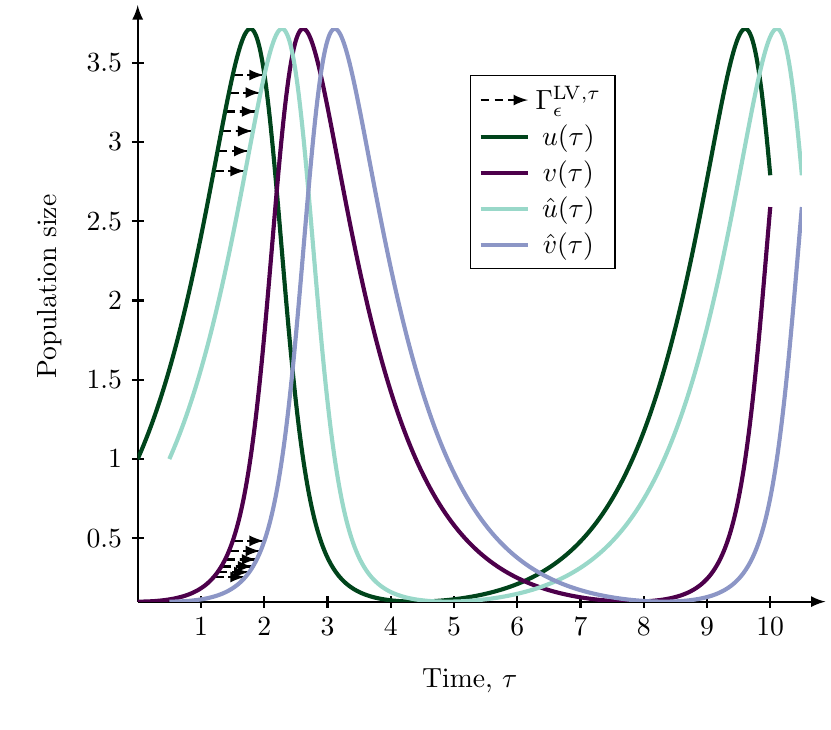
\begin{tikzpicture}
  % The axis of the plot
\begin{axis}[
    xlabel={Time, $\tau$},
    ylabel={Population size},
    x label style={at={(axis description cs:0.5,-0.1)},anchor=north},
    y label style={at={(axis description cs:-0.1,0.55)},rotate=90,anchor=south},
    scaled x ticks = false,
    legend style={at={(axis description cs:0.5,0.75)},anchor=west,nodes={scale=1.00, transform shape}},    
    grid style=dashed,
]
\addplot[
color=black,->,>=latex,densely dashed
]
coordinates {%
(1.2024048096192383,nan)
(1.2124048096192384,2.8173084568794162)
(1.2224048096192384,2.8173084568794162)
(1.2324048096192384,2.8173084568794162)
(1.2424048096192384,2.8173084568794162)
(1.2524048096192384,2.8173084568794162)
(1.2624048096192384,2.8173084568794162)
(1.2724048096192384,2.8173084568794162)
(1.2824048096192384,2.8173084568794162)
(1.2924048096192384,2.8173084568794162)
(1.3024048096192384,2.8173084568794162)
(1.3124048096192384,2.8173084568794162)
(1.3224048096192385,2.8173084568794162)
(1.3324048096192382,2.8173084568794162)
(1.3424048096192385,2.8173084568794162)
(1.3524048096192383,2.8173084568794162)
(1.3624048096192383,2.8173084568794162)
(1.3724048096192383,2.8173084568794162)
(1.3824048096192383,2.8173084568794162)
(1.3924048096192383,2.8173084568794162)
(1.4024048096192383,2.8173084568794162)
(1.4124048096192383,2.8173084568794162)
(1.4224048096192383,2.8173084568794162)
(1.4324048096192383,2.8173084568794162)
(1.4424048096192383,2.8173084568794162)
(1.4524048096192383,2.8173084568794162)
(1.4624048096192384,2.8173084568794162)
(1.4724048096192384,2.8173084568794162)
(1.4824048096192384,2.8173084568794162)
(1.4924048096192384,2.8173084568794162)
(1.5024048096192384,2.8173084568794162)
(1.5124048096192384,2.8173084568794162)
(1.5224048096192384,2.8173084568794162)
(1.5324048096192384,2.8173084568794162)
(1.5424048096192384,2.8173084568794162)
(1.5524048096192384,2.8173084568794162)
(1.5624048096192382,2.8173084568794162)
(1.5724048096192385,2.8173084568794162)
(1.5824048096192382,2.8173084568794162)
(1.5924048096192385,2.8173084568794162)
(1.6024048096192383,2.8173084568794162)
(1.6124048096192385,2.8173084568794162)
(1.6224048096192383,2.8173084568794162)
(1.6324048096192383,2.8173084568794162)
(1.6424048096192383,2.8173084568794162)
(1.6524048096192383,2.8173084568794162)
(1.6624048096192383,2.8173084568794162)
(1.6724048096192383,2.8173084568794162)
(1.6824048096192383,2.8173084568794162)
(1.6924048096192383,2.8173084568794162)
};
\addlegendentry{$\Gamma^{\mathrm{LV},\tau}_{\epsilon}$}
\addplot[
forget plot,
color=black,->,>=latex,densely dashed
]
coordinates {%
(1.2024048096192383,nan)
(1.2124048096192384,0.2551487208308566)
(1.2224048096192384,0.2551487208308566)
(1.2324048096192384,0.2551487208308566)
(1.2424048096192384,0.2551487208308566)
(1.2524048096192384,0.2551487208308566)
(1.2624048096192384,0.2551487208308566)
(1.2724048096192384,0.2551487208308566)
(1.2824048096192384,0.2551487208308566)
(1.2924048096192384,0.2551487208308566)
(1.3024048096192384,0.2551487208308566)
(1.3124048096192384,0.2551487208308566)
(1.3224048096192385,0.2551487208308566)
(1.3324048096192382,0.2551487208308566)
(1.3424048096192385,0.2551487208308566)
(1.3524048096192383,0.2551487208308566)
(1.3624048096192383,0.2551487208308566)
(1.3724048096192383,0.2551487208308566)
(1.3824048096192383,0.2551487208308566)
(1.3924048096192383,0.2551487208308566)
(1.4024048096192383,0.2551487208308566)
(1.4124048096192383,0.2551487208308566)
(1.4224048096192383,0.2551487208308566)
(1.4324048096192383,0.2551487208308566)
(1.4424048096192383,0.2551487208308566)
(1.4524048096192383,0.2551487208308566)
(1.4624048096192384,0.2551487208308566)
(1.4724048096192384,0.2551487208308566)
(1.4824048096192384,0.2551487208308566)
(1.4924048096192384,0.2551487208308566)
(1.5024048096192384,0.2551487208308566)
(1.5124048096192384,0.2551487208308566)
(1.5224048096192384,0.2551487208308566)
(1.5324048096192384,0.2551487208308566)
(1.5424048096192384,0.2551487208308566)
(1.5524048096192384,0.2551487208308566)
(1.5624048096192382,0.2551487208308566)
(1.5724048096192385,0.2551487208308566)
(1.5824048096192382,0.2551487208308566)
(1.5924048096192385,0.2551487208308566)
(1.6024048096192383,0.2551487208308566)
(1.6124048096192385,0.2551487208308566)
(1.6224048096192383,0.2551487208308566)
(1.6324048096192383,0.2551487208308566)
(1.6424048096192383,0.2551487208308566)
(1.6524048096192383,0.2551487208308566)
(1.6624048096192383,0.2551487208308566)
(1.6724048096192383,0.2551487208308566)
(1.6824048096192383,0.2551487208308566)
(1.6924048096192383,0.2551487208308566)
};
\addplot[
forget plot,
color=black,->,>=latex,densely dashed
]
coordinates {%
(1.2625250501002003,nan)
(1.2725250501002003,2.9437143206651966)
(1.2825250501002003,2.9437143206651966)
(1.2925250501002004,2.943714320665196)
(1.3025250501002004,2.9437143206651966)
(1.3125250501002004,2.9437143206651966)
(1.3225250501002004,2.943714320665196)
(1.3325250501002004,2.9437143206651966)
(1.3425250501002004,2.9437143206651966)
(1.3525250501002004,2.9437143206651966)
(1.3625250501002004,2.9437143206651966)
(1.3725250501002004,2.9437143206651966)
(1.3825250501002002,2.943714320665196)
(1.3925250501002004,2.9437143206651966)
(1.4025250501002002,2.9437143206651966)
(1.4125250501002002,2.9437143206651966)
(1.4225250501002003,2.9437143206651966)
(1.4325250501002003,2.9437143206651966)
(1.4425250501002003,2.9437143206651966)
(1.4525250501002003,2.9437143206651966)
(1.4625250501002003,2.9437143206651966)
(1.4725250501002003,2.9437143206651966)
(1.4825250501002003,2.9437143206651966)
(1.4925250501002003,2.9437143206651966)
(1.5025250501002003,2.943714320665196)
(1.5125250501002003,2.9437143206651966)
(1.5225250501002003,2.9437143206651966)
(1.5325250501002003,2.9437143206651966)
(1.5425250501002004,2.9437143206651966)
(1.5525250501002004,2.9437143206651966)
(1.5625250501002004,2.9437143206651966)
(1.5725250501002004,2.9437143206651966)
(1.5825250501002004,2.9437143206651966)
(1.5925250501002004,2.9437143206651966)
(1.6025250501002004,2.9437143206651966)
(1.6125250501002004,2.9437143206651966)
(1.6225250501002004,2.9437143206651966)
(1.6325250501002002,2.9437143206651966)
(1.6425250501002004,2.9437143206651966)
(1.6525250501002002,2.9437143206651966)
(1.6625250501002005,2.9437143206651966)
(1.6725250501002003,2.9437143206651966)
(1.6825250501002003,2.9437143206651966)
(1.6925250501002003,2.9437143206651966)
(1.7025250501002003,2.9437143206651966)
(1.7125250501002003,2.9437143206651966)
(1.7225250501002003,2.9437143206651966)
(1.7325250501002003,2.9437143206651966)
(1.7425250501002003,2.943714320665196)
(1.7525250501002003,2.9437143206651966)
};
\addplot[
forget plot,
color=black,->,>=latex,densely dashed
]
coordinates {%
(1.2625250501002003,nan)
(1.2725250501002003,0.2856885142698433)
(1.2825250501002003,0.2856885142698433)
(1.2925250501002004,0.2856885142698433)
(1.3025250501002004,0.2856885142698433)
(1.3125250501002004,0.2856885142698433)
(1.3225250501002004,0.2856885142698433)
(1.3325250501002004,0.2856885142698433)
(1.3425250501002004,0.2856885142698433)
(1.3525250501002004,0.2856885142698433)
(1.3625250501002004,0.2856885142698433)
(1.3725250501002004,0.2856885142698433)
(1.3825250501002002,0.2856885142698433)
(1.3925250501002004,0.2856885142698433)
(1.4025250501002002,0.2856885142698433)
(1.4125250501002002,0.2856885142698433)
(1.4225250501002003,0.2856885142698433)
(1.4325250501002003,0.2856885142698433)
(1.4425250501002003,0.2856885142698433)
(1.4525250501002003,0.2856885142698433)
(1.4625250501002003,0.2856885142698433)
(1.4725250501002003,0.2856885142698433)
(1.4825250501002003,0.2856885142698433)
(1.4925250501002003,0.2856885142698433)
(1.5025250501002003,0.2856885142698433)
(1.5125250501002003,0.2856885142698433)
(1.5225250501002003,0.2856885142698433)
(1.5325250501002003,0.2856885142698433)
(1.5425250501002004,0.2856885142698433)
(1.5525250501002004,0.2856885142698433)
(1.5625250501002004,0.2856885142698433)
(1.5725250501002004,0.2856885142698433)
(1.5825250501002004,0.2856885142698433)
(1.5925250501002004,0.2856885142698433)
(1.6025250501002004,0.2856885142698433)
(1.6125250501002004,0.2856885142698433)
(1.6225250501002004,0.2856885142698433)
(1.6325250501002002,0.2856885142698433)
(1.6425250501002004,0.2856885142698433)
(1.6525250501002002,0.2856885142698433)
(1.6625250501002005,0.2856885142698433)
(1.6725250501002003,0.2856885142698433)
(1.6825250501002003,0.2856885142698433)
(1.6925250501002003,0.2856885142698433)
(1.7025250501002003,0.2856885142698433)
(1.7125250501002003,0.2856885142698433)
(1.7225250501002003,0.2856885142698433)
(1.7325250501002003,0.2856885142698433)
(1.7425250501002003,0.2856885142698433)
(1.7525250501002003,0.2856885142698433)
};
\addplot[
forget plot,
color=black,->,>=latex,densely dashed
]
coordinates {%
(1.3226452905811623,nan)
(1.3326452905811623,3.0696059555025323)
(1.3426452905811623,3.0696059555025323)
(1.3526452905811623,3.069605955502533)
(1.3626452905811623,3.0696059555025323)
(1.3726452905811624,3.0696059555025323)
(1.3826452905811624,3.069605955502533)
(1.3926452905811624,3.0696059555025323)
(1.4026452905811624,3.0696059555025323)
(1.4126452905811624,3.0696059555025323)
(1.4226452905811624,3.0696059555025323)
(1.4326452905811624,3.069605955502532)
(1.4426452905811624,3.069605955502533)
(1.4526452905811622,3.0696059555025323)
(1.4626452905811624,3.0696059555025323)
(1.4726452905811622,3.0696059555025323)
(1.4826452905811622,3.0696059555025323)
(1.4926452905811622,3.0696059555025323)
(1.5026452905811623,3.0696059555025323)
(1.5126452905811623,3.0696059555025323)
(1.5226452905811623,3.0696059555025323)
(1.5326452905811623,3.0696059555025323)
(1.5426452905811623,3.069605955502532)
(1.5526452905811623,3.0696059555025323)
(1.5626452905811623,3.069605955502533)
(1.5726452905811623,3.0696059555025323)
(1.5826452905811623,3.0696059555025323)
(1.5926452905811623,3.0696059555025323)
(1.6026452905811623,3.0696059555025323)
(1.6126452905811623,3.0696059555025323)
(1.6226452905811624,3.0696059555025323)
(1.6326452905811624,3.0696059555025323)
(1.6426452905811624,3.0696059555025323)
(1.6526452905811624,3.0696059555025323)
(1.6626452905811624,3.0696059555025323)
(1.6726452905811624,3.0696059555025323)
(1.6826452905811622,3.0696059555025323)
(1.6926452905811624,3.0696059555025323)
(1.7026452905811622,3.0696059555025323)
(1.7126452905811624,3.0696059555025323)
(1.7226452905811622,3.0696059555025323)
(1.7326452905811625,3.0696059555025323)
(1.7426452905811622,3.0696059555025323)
(1.7526452905811623,3.069605955502533)
(1.7626452905811623,3.069605955502532)
(1.7726452905811623,3.0696059555025323)
(1.7826452905811623,3.0696059555025323)
(1.7926452905811623,3.0696059555025323)
(1.8026452905811623,3.069605955502533)
(1.8126452905811623,3.0696059555025323)
};
\addplot[
forget plot,
color=black,->,>=latex,densely dashed
]
coordinates {%
(1.3226452905811623,nan)
(1.3326452905811623,0.32232155791556755)
(1.3426452905811623,0.32232155791556755)
(1.3526452905811623,0.32232155791556755)
(1.3626452905811623,0.32232155791556755)
(1.3726452905811624,0.32232155791556755)
(1.3826452905811624,0.32232155791556755)
(1.3926452905811624,0.32232155791556755)
(1.4026452905811624,0.32232155791556755)
(1.4126452905811624,0.32232155791556755)
(1.4226452905811624,0.32232155791556755)
(1.4326452905811624,0.32232155791556755)
(1.4426452905811624,0.32232155791556755)
(1.4526452905811622,0.32232155791556755)
(1.4626452905811624,0.32232155791556755)
(1.4726452905811622,0.32232155791556755)
(1.4826452905811622,0.32232155791556755)
(1.4926452905811622,0.32232155791556755)
(1.5026452905811623,0.32232155791556755)
(1.5126452905811623,0.32232155791556755)
(1.5226452905811623,0.32232155791556755)
(1.5326452905811623,0.32232155791556755)
(1.5426452905811623,0.32232155791556755)
(1.5526452905811623,0.32232155791556755)
(1.5626452905811623,0.32232155791556755)
(1.5726452905811623,0.32232155791556755)
(1.5826452905811623,0.32232155791556755)
(1.5926452905811623,0.32232155791556755)
(1.6026452905811623,0.32232155791556755)
(1.6126452905811623,0.32232155791556755)
(1.6226452905811624,0.32232155791556755)
(1.6326452905811624,0.32232155791556755)
(1.6426452905811624,0.32232155791556755)
(1.6526452905811624,0.32232155791556755)
(1.6626452905811624,0.32232155791556755)
(1.6726452905811624,0.32232155791556755)
(1.6826452905811622,0.32232155791556755)
(1.6926452905811624,0.32232155791556755)
(1.7026452905811622,0.32232155791556755)
(1.7126452905811624,0.32232155791556755)
(1.7226452905811622,0.32232155791556755)
(1.7326452905811625,0.32232155791556755)
(1.7426452905811622,0.32232155791556755)
(1.7526452905811623,0.32232155791556755)
(1.7626452905811623,0.32232155791556755)
(1.7726452905811623,0.32232155791556755)
(1.7826452905811623,0.32232155791556755)
(1.7926452905811623,0.32232155791556755)
(1.8026452905811623,0.32232155791556755)
(1.8126452905811623,0.32232155791556755)
};
\addplot[
forget plot,
color=black,->,>=latex,densely dashed
]
coordinates {%
(1.3827655310621243,nan)
(1.3927655310621243,3.1931493541965215)
(1.4027655310621243,3.1931493541965215)
(1.4127655310621243,3.1931493541965215)
(1.4227655310621243,3.1931493541965215)
(1.4327655310621243,3.1931493541965215)
(1.4427655310621244,3.1931493541965215)
(1.4527655310621244,3.1931493541965215)
(1.4627655310621244,3.1931493541965215)
(1.4727655310621244,3.1931493541965215)
(1.4827655310621244,3.1931493541965215)
(1.4927655310621244,3.1931493541965215)
(1.5027655310621242,3.1931493541965215)
(1.5127655310621244,3.1931493541965215)
(1.5227655310621242,3.1931493541965215)
(1.5327655310621242,3.1931493541965215)
(1.5427655310621242,3.1931493541965215)
(1.5527655310621242,3.1931493541965215)
(1.5627655310621242,3.1931493541965215)
(1.5727655310621242,3.1931493541965215)
(1.5827655310621243,3.1931493541965215)
(1.5927655310621243,3.193149354196522)
(1.6027655310621243,3.1931493541965215)
(1.6127655310621243,3.1931493541965215)
(1.6227655310621243,3.1931493541965215)
(1.6327655310621243,3.1931493541965215)
(1.6427655310621243,3.1931493541965215)
(1.6527655310621243,3.1931493541965215)
(1.6627655310621243,3.1931493541965215)
(1.6727655310621243,3.1931493541965215)
(1.6827655310621243,3.1931493541965215)
(1.6927655310621244,3.1931493541965215)
(1.7027655310621244,3.1931493541965215)
(1.7127655310621244,3.1931493541965215)
(1.7227655310621244,3.1931493541965215)
(1.7327655310621244,3.1931493541965215)
(1.7427655310621244,3.1931493541965215)
(1.7527655310621242,3.1931493541965215)
(1.7627655310621244,3.1931493541965215)
(1.7727655310621242,3.1931493541965215)
(1.7827655310621244,3.1931493541965215)
(1.7927655310621242,3.193149354196522)
(1.8027655310621242,3.193149354196522)
(1.8127655310621242,3.1931493541965215)
(1.8227655310621242,3.1931493541965215)
(1.8327655310621243,3.1931493541965215)
(1.8427655310621243,3.1931493541965215)
(1.8527655310621243,3.1931493541965215)
(1.8627655310621243,3.1931493541965215)
(1.8727655310621243,3.1931493541965215)
};
\addplot[
forget plot,
color=black,->,>=latex,densely dashed
]
coordinates {%
(1.3827655310621243,nan)
(1.3927655310621243,0.3663927037123817)
(1.4027655310621243,0.3663927037123817)
(1.4127655310621243,0.3663927037123817)
(1.4227655310621243,0.3663927037123817)
(1.4327655310621243,0.3663927037123817)
(1.4427655310621244,0.3663927037123817)
(1.4527655310621244,0.3663927037123817)
(1.4627655310621244,0.3663927037123817)
(1.4727655310621244,0.3663927037123817)
(1.4827655310621244,0.3663927037123817)
(1.4927655310621244,0.36639270371238175)
(1.5027655310621242,0.3663927037123817)
(1.5127655310621244,0.3663927037123817)
(1.5227655310621242,0.3663927037123817)
(1.5327655310621242,0.3663927037123817)
(1.5427655310621242,0.3663927037123817)
(1.5527655310621242,0.3663927037123817)
(1.5627655310621242,0.3663927037123817)
(1.5727655310621242,0.3663927037123817)
(1.5827655310621243,0.3663927037123817)
(1.5927655310621243,0.3663927037123817)
(1.6027655310621243,0.36639270371238175)
(1.6127655310621243,0.36639270371238164)
(1.6227655310621243,0.3663927037123817)
(1.6327655310621243,0.3663927037123817)
(1.6427655310621243,0.3663927037123817)
(1.6527655310621243,0.3663927037123817)
(1.6627655310621243,0.3663927037123817)
(1.6727655310621243,0.36639270371238164)
(1.6827655310621243,0.3663927037123817)
(1.6927655310621244,0.3663927037123817)
(1.7027655310621244,0.3663927037123817)
(1.7127655310621244,0.3663927037123817)
(1.7227655310621244,0.3663927037123817)
(1.7327655310621244,0.3663927037123817)
(1.7427655310621244,0.3663927037123817)
(1.7527655310621242,0.3663927037123817)
(1.7627655310621244,0.3663927037123817)
(1.7727655310621242,0.3663927037123817)
(1.7827655310621244,0.3663927037123817)
(1.7927655310621242,0.3663927037123817)
(1.8027655310621242,0.3663927037123817)
(1.8127655310621242,0.3663927037123817)
(1.8227655310621242,0.36639270371238175)
(1.8327655310621243,0.36639270371238164)
(1.8427655310621243,0.36639270371238164)
(1.8527655310621243,0.3663927037123817)
(1.8627655310621243,0.3663927037123817)
(1.8727655310621243,0.3663927037123817)
};
\addplot[
forget plot,
color=black,->,>=latex,densely dashed
]
coordinates {%
(1.442885771543086,nan)
(1.452885771543086,3.312001757563654)
(1.462885771543086,3.312001757563654)
(1.472885771543086,3.3120017575636544)
(1.482885771543086,3.312001757563654)
(1.492885771543086,3.312001757563654)
(1.5028857715430861,3.3120017575636544)
(1.5128857715430861,3.312001757563654)
(1.5228857715430861,3.312001757563654)
(1.5328857715430861,3.312001757563654)
(1.5428857715430861,3.312001757563654)
(1.5528857715430862,3.312001757563654)
(1.562885771543086,3.3120017575636544)
(1.5728857715430862,3.312001757563654)
(1.582885771543086,3.312001757563654)
(1.592885771543086,3.312001757563654)
(1.602885771543086,3.312001757563654)
(1.612885771543086,3.312001757563654)
(1.622885771543086,3.312001757563654)
(1.632885771543086,3.312001757563654)
(1.642885771543086,3.312001757563654)
(1.652885771543086,3.3120017575636544)
(1.662885771543086,3.312001757563654)
(1.672885771543086,3.312001757563654)
(1.682885771543086,3.3120017575636544)
(1.692885771543086,3.312001757563654)
(1.702885771543086,3.312001757563654)
(1.712885771543086,3.3120017575636536)
(1.722885771543086,3.312001757563654)
(1.732885771543086,3.312001757563654)
(1.742885771543086,3.312001757563654)
(1.7528857715430861,3.312001757563654)
(1.7628857715430861,3.312001757563654)
(1.7728857715430861,3.312001757563654)
(1.7828857715430861,3.312001757563654)
(1.7928857715430861,3.312001757563654)
(1.8028857715430862,3.312001757563654)
(1.812885771543086,3.312001757563654)
(1.8228857715430862,3.312001757563654)
(1.832885771543086,3.312001757563654)
(1.8428857715430862,3.312001757563654)
(1.852885771543086,3.3120017575636536)
(1.862885771543086,3.3120017575636544)
(1.872885771543086,3.312001757563654)
(1.882885771543086,3.312001757563654)
(1.892885771543086,3.312001757563654)
(1.902885771543086,3.312001757563654)
(1.912885771543086,3.312001757563654)
(1.922885771543086,3.3120017575636544)
(1.932885771543086,3.312001757563654)
};
\addplot[
forget plot,
color=black,->,>=latex,densely dashed
]
coordinates {%
(1.442885771543086,nan)
(1.452885771543086,0.4195410438530903)
(1.462885771543086,0.4195410438530903)
(1.472885771543086,0.4195410438530904)
(1.482885771543086,0.4195410438530903)
(1.492885771543086,0.4195410438530903)
(1.5028857715430861,0.4195410438530904)
(1.5128857715430861,0.4195410438530903)
(1.5228857715430861,0.4195410438530903)
(1.5328857715430861,0.4195410438530903)
(1.5428857715430861,0.4195410438530903)
(1.5528857715430862,0.4195410438530903)
(1.562885771543086,0.4195410438530904)
(1.5728857715430862,0.4195410438530903)
(1.582885771543086,0.4195410438530903)
(1.592885771543086,0.4195410438530903)
(1.602885771543086,0.4195410438530903)
(1.612885771543086,0.4195410438530903)
(1.622885771543086,0.4195410438530903)
(1.632885771543086,0.4195410438530903)
(1.642885771543086,0.4195410438530903)
(1.652885771543086,0.4195410438530903)
(1.662885771543086,0.4195410438530903)
(1.672885771543086,0.4195410438530903)
(1.682885771543086,0.4195410438530904)
(1.692885771543086,0.4195410438530903)
(1.702885771543086,0.4195410438530903)
(1.712885771543086,0.4195410438530903)
(1.722885771543086,0.4195410438530903)
(1.732885771543086,0.4195410438530903)
(1.742885771543086,0.4195410438530903)
(1.7528857715430861,0.4195410438530903)
(1.7628857715430861,0.4195410438530903)
(1.7728857715430861,0.4195410438530903)
(1.7828857715430861,0.4195410438530903)
(1.7928857715430861,0.4195410438530903)
(1.8028857715430862,0.4195410438530903)
(1.812885771543086,0.4195410438530903)
(1.8228857715430862,0.4195410438530903)
(1.832885771543086,0.41954104385309027)
(1.8428857715430862,0.4195410438530903)
(1.852885771543086,0.4195410438530903)
(1.862885771543086,0.4195410438530903)
(1.872885771543086,0.4195410438530903)
(1.882885771543086,0.4195410438530903)
(1.892885771543086,0.4195410438530903)
(1.902885771543086,0.4195410438530903)
(1.912885771543086,0.4195410438530904)
(1.922885771543086,0.4195410438530904)
(1.932885771543086,0.41954104385309027)
};
\addplot[
forget plot,
color=black,->,>=latex,densely dashed
]
coordinates {%
(1.503006012024048,nan)
(1.513006012024048,3.4232183117111905)
(1.523006012024048,3.4232183117111905)
(1.533006012024048,3.4232183117111905)
(1.543006012024048,3.4232183117111905)
(1.553006012024048,3.42321831171119)
(1.563006012024048,3.4232183117111905)
(1.573006012024048,3.423218311711191)
(1.5830060120240481,3.4232183117111905)
(1.5930060120240481,3.4232183117111905)
(1.6030060120240481,3.42321831171119)
(1.6130060120240481,3.4232183117111905)
(1.6230060120240482,3.4232183117111905)
(1.633006012024048,3.4232183117111905)
(1.6430060120240482,3.423218311711191)
(1.653006012024048,3.4232183117111905)
(1.663006012024048,3.4232183117111905)
(1.673006012024048,3.4232183117111905)
(1.683006012024048,3.4232183117111905)
(1.693006012024048,3.4232183117111905)
(1.703006012024048,3.42321831171119)
(1.713006012024048,3.4232183117111905)
(1.723006012024048,3.4232183117111905)
(1.733006012024048,3.42321831171119)
(1.743006012024048,3.4232183117111905)
(1.753006012024048,3.4232183117111905)
(1.763006012024048,3.4232183117111905)
(1.773006012024048,3.4232183117111905)
(1.783006012024048,3.423218311711191)
(1.793006012024048,3.4232183117111905)
(1.803006012024048,3.4232183117111905)
(1.813006012024048,3.4232183117111905)
(1.823006012024048,3.4232183117111905)
(1.8330060120240481,3.4232183117111905)
(1.8430060120240481,3.4232183117111905)
(1.8530060120240481,3.4232183117111905)
(1.863006012024048,3.4232183117111905)
(1.8730060120240482,3.4232183117111905)
(1.883006012024048,3.4232183117111905)
(1.8930060120240482,3.423218311711191)
(1.903006012024048,3.42321831171119)
(1.9130060120240482,3.4232183117111905)
(1.923006012024048,3.4232183117111905)
(1.933006012024048,3.4232183117111905)
(1.943006012024048,3.4232183117111905)
(1.953006012024048,3.423218311711191)
(1.963006012024048,3.42321831171119)
(1.973006012024048,3.4232183117111905)
(1.983006012024048,3.4232183117111905)
(1.993006012024048,3.4232183117111905)
};
\addplot[
forget plot,
color=black,->,>=latex,densely dashed
]
coordinates {%
(1.503006012024048,nan)
(1.513006012024048,0.4837408261662278)
(1.523006012024048,0.4837408261662278)
(1.533006012024048,0.48374082616622777)
(1.543006012024048,0.4837408261662278)
(1.553006012024048,0.4837408261662278)
(1.563006012024048,0.48374082616622777)
(1.573006012024048,0.4837408261662278)
(1.5830060120240481,0.4837408261662278)
(1.5930060120240481,0.4837408261662278)
(1.6030060120240481,0.4837408261662278)
(1.6130060120240481,0.4837408261662279)
(1.6230060120240482,0.48374082616622777)
(1.633006012024048,0.4837408261662278)
(1.6430060120240482,0.4837408261662278)
(1.653006012024048,0.4837408261662278)
(1.663006012024048,0.4837408261662278)
(1.673006012024048,0.4837408261662278)
(1.683006012024048,0.4837408261662278)
(1.693006012024048,0.4837408261662278)
(1.703006012024048,0.4837408261662278)
(1.713006012024048,0.4837408261662278)
(1.723006012024048,0.4837408261662279)
(1.733006012024048,0.4837408261662279)
(1.743006012024048,0.48374082616622777)
(1.753006012024048,0.48374082616622777)
(1.763006012024048,0.4837408261662278)
(1.773006012024048,0.4837408261662278)
(1.783006012024048,0.4837408261662278)
(1.793006012024048,0.4837408261662278)
(1.803006012024048,0.4837408261662278)
(1.813006012024048,0.4837408261662278)
(1.823006012024048,0.4837408261662278)
(1.8330060120240481,0.4837408261662278)
(1.8430060120240481,0.4837408261662278)
(1.8530060120240481,0.48374082616622777)
(1.863006012024048,0.4837408261662278)
(1.8730060120240482,0.48374082616622777)
(1.883006012024048,0.4837408261662278)
(1.8930060120240482,0.4837408261662278)
(1.903006012024048,0.4837408261662278)
(1.9130060120240482,0.4837408261662278)
(1.923006012024048,0.4837408261662278)
(1.933006012024048,0.4837408261662278)
(1.943006012024048,0.4837408261662279)
(1.953006012024048,0.4837408261662278)
(1.963006012024048,0.4837408261662279)
(1.973006012024048,0.4837408261662278)
(1.983006012024048,0.48374082616622777)
(1.993006012024048,0.4837408261662278)
};
\addplot[
color=clr_1,line width=1.5pt,
]
coordinates {%
(0.0,1.0)
(0.02004008016032064,1.0181996110300777)
(0.04008016032064128,1.0367296106909476)
(0.06012024048096192,1.055595323632852)
(0.08016032064128256,1.074801937002425)
(0.1002004008016032,1.0943547160918659)
(0.12024048096192384,1.1142589534321468)
(0.1402805611222445,1.1345199679569662)
(0.16032064128256512,1.1551430945650516)
(0.18036072144288576,1.1761336872879984)
(0.2004008016032064,1.1974971035842958)
(0.22044088176352705,1.2192387061207308)
(0.24048096192384769,1.2413638558986257)
(0.2605210420841683,1.2638778999901288)
(0.280561122244489,1.2867861736913744)
(0.3006012024048096,1.3100939785635095)
(0.32064128256513025,1.3338065915666082)
(0.3406813627254509,1.3579292461915127)
(0.3607214428857715,1.382467112166135)
(0.3807615230460922,1.4074252938862326)
(0.4008016032064128,1.4328088196709685)
(0.42084168336673344,1.4586226291994238)
(0.4408817635270541,1.4848715582100407)
(0.4609218436873747,1.5115603131552386)
(0.48096192384769537,1.5386934682102975)
(0.501002004008016,1.56627544150381)
(0.5210420841683366,1.5943104653061733)
(0.5410821643286573,1.622802585086228)
(0.561122244488978,1.6517556163611076)
(0.5811623246492986,1.6811731270259525)
(0.6012024048096192,1.7110584212925342)
(0.6212424849699398,1.7414144829451266)
(0.6412825651302605,1.772243970481731)
(0.6613226452905812,1.8035491749082546)
(0.6813627254509018,1.8353319612447034)
(0.7014028056112224,1.867593766913634)
(0.721442885771543,1.9003355226998437)
(0.7414829659318637,1.9335576154267315)
(0.7615230460921844,1.967259861251073)
(0.781563126252505,2.00144139885065)
(0.8016032064128256,2.0361006772105634)
(0.8216432865731462,2.0712353852431153)
(0.8416833667334669,2.1068423369363294)
(0.8617234468937875,2.1429174452044726)
(0.8817635270541082,2.1794556098768134)
(0.9018036072144289,2.216450659688801)
(0.9218436873747494,2.2538952186695282)
(0.9418837675350701,2.2917806319558793)
(0.9619238476953907,2.330096838779097)
(0.9819639278557114,2.368832252375849)
(1.002004008016032,2.4079736481061227)
(1.0220440881763526,2.4475059848649012)
(1.0420841683366733,2.4874123111638315)
(1.062124248496994,2.5276735327655238)
(1.0821643286573146,2.5682683152263577)
(1.1022044088176353,2.6091728206480704)
(1.122244488977956,2.650360574870958)
(1.1422845691382766,2.6918022006186266)
(1.1623246492985972,2.733465214053031)
(1.1823647294589177,2.775313793127582)
(1.2024048096192383,2.8173084568794162)
(1.222444889779559,2.859405885537604)
(1.2424849699398797,2.901558515023622)
(1.2625250501002003,2.9437143206651966)
(1.282565130260521,2.9858164480671148)
(1.3026052104208417,3.0278028536258987)
(1.3226452905811623,3.0696059555025323)
(1.342685370741483,3.111152324243746)
(1.3627254509018036,3.15236225137405)
(1.3827655310621243,3.1931493541965215)
(1.4028056112224447,3.2334201912020424)
(1.4228456913827654,3.2730738950230225)
(1.442885771543086,3.312001757563654)
(1.4629258517034067,3.350086888283124)
(1.4829659318637274,3.387203834460446)
(1.503006012024048,3.4232183117111905)
(1.5230460921843687,3.457986883991823)
(1.5430861723446894,3.4913568299320348)
(1.56312625250501,3.5231659300207308)
(1.5831663326653307,3.553242540113277)
(1.6032064128256511,3.581405638028455)
(1.6232464929859718,3.6074650564007062)
(1.6432865731462925,3.6312219325940935)
(1.6633266533066131,3.652469310039041)
(1.6833667334669338,3.6709930261045214)
(1.7034068136272544,3.686572798684044)
(1.723446893787575,3.6989836792207047)
(1.7434869739478958,3.7079977928400676)
(1.7635270541082164,3.7133864264845857)
(1.783567134268537,3.7149225373146835)
(1.8036072144288577,3.712383573299039)
(1.8236472945891782,3.7055547526917274)
(1.8436873747494988,3.694232652635815)
(1.8637274549098195,3.6782291912857836)
(1.8837675350701402,3.657375838918677)
(1.9038076152304608,3.631528116607061)
(1.9238476953907815,3.6005701472650298)
(1.9438877755511021,3.564419247258668)
(1.9639278557114228,3.523030260185355)
(1.9839679358717435,3.4763997955228843)
(2.004008016032064,3.424569728349855)
(2.024048096192385,3.3676301594765565)
(2.0440881763527052,3.305721482108544)
(2.064128256513026,3.2390353870850834)
(2.0841683366733466,3.1678147114973596)
(2.1042084168336674,3.0923520249742493)
(2.124248496993988,3.0129868711372794)
(2.1442885771543083,2.9301016836553053)
(2.164328657314629,2.844116477521267)
(2.1843687374749496,2.7554824208200257)
(2.2044088176352705,2.6646744793866937)
(2.224448897795591,2.5721834116423103)
(2.244488977955912,2.4785073974533534)
(2.2645290581162323,2.38414354871953)
(2.284569138276553,2.289579654287321)
(2.3046092184368736,2.1952864569614197)
(2.3246492985971945,2.1017106887169765)
(2.344689378757515,2.0092690289430606)
(2.3647294589178354,1.9183432004123362)
(2.3847695390781563,1.8292762657323478)
(2.4048096192384767,1.7423701224156958)
(2.4248496993987976,1.6578841746791864)
(2.444889779559118,1.5760351139000683)
(2.464929859719439,1.4969977505087715)
(2.4849699398797593,1.420906547640438)
(2.50501002004008,1.3478579312616616)
(2.5250501002004007,1.2779132031145086)
(2.5450901803607215,1.211101634341837)
(2.565130260521042,1.1474239328597449)
(2.5851703406813624,1.086855748273381)
(2.6052104208416833,1.0293511605567924)
(2.6252505010020037,0.9748460571069857)
(2.6452905811623246,0.9232613488697714)
(2.665330661322645,0.8745059539098055)
(2.685370741482966,0.8284795187162423)
(2.7054108216432864,0.7850748605408029)
(2.7254509018036073,0.7441801319492899)
(2.7454909819639277,0.7056807030954716)
(2.7655310621242486,0.6694607709981598)
(2.785571142284569,0.6354047241687562)
(2.8056112224448895,0.6033982625444894)
(2.8256513026052104,0.5733293202438954)
(2.845691382765531,0.5450887993091171)
(2.8657314629258517,0.5185711135951477)
(2.885771543086172,0.4936746370828911)
(2.905811623246493,0.47030197368957394)
(2.9258517034068134,0.4483601624437748)
(2.9458917835671343,0.4277607852697122)
(2.9659318637274548,0.4084199830625315)
(2.9859719438877756,0.39025845204702037)
(3.006012024048096,0.37320135314094605)
(3.0260521042084165,0.35717821015222967)
(3.0460921843687374,0.3421227766463634)
(3.066132264529058,0.32797286837066253)
(3.0861723446893787,0.314670203264955)
(3.106212424849699,0.3021602123505395)
(3.12625250501002,0.290391856169708)
(3.1462925851703405,0.2793174397034971)
(3.1663326653306614,0.2688924218059914)
(3.186372745490982,0.2590752340953084)
(3.2064128256513023,0.24982709846963916)
(3.226452905811623,0.2411118605391948)
(3.2464929859719436,0.23289581781992433)
(3.2665330661322645,0.22514756275722989)
(3.286573146292585,0.21783783134532678)
(3.306613226452906,0.21093935976361497)
(3.3266533066132262,0.20442674907953734)
(3.346693386773547,0.19827633758309587)
(3.3667334669338675,0.19246608102168825)
(3.3867735470941884,0.18697544051326784)
(3.406813627254509,0.1817852769554324)
(3.4268537074148293,0.17687775306775538)
(3.44689378757515,0.17223624065453536)
(3.4669338677354706,0.16784524002950393)
(3.4869739478957915,0.16369029642707708)
(3.507014028056112,0.15975792127784433)
(3.527054108216433,0.15603553645926793)
(3.5470941883767533,0.15251140043451053)
(3.567134268537074,0.14917454683223103)
(3.5871743486973946,0.14601474260862798)
(3.6072144288577155,0.14302242437038218)
(3.627254509018036,0.14018865303319103)
(3.6472945891783564,0.13750508000830508)
(3.6673346693386772,0.13496389371521256)
(3.6873747494989977,0.13255778713414743)
(3.7074148296593186,0.13027992927065288)
(3.727454909819639,0.12812392109630114)
(3.74749498997996,0.12608377271367066)
(3.7675350701402803,0.12415387878012203)
(3.787575150300601,0.12232898285201395)
(3.8076152304609217,0.12060416134370619)
(3.8276553106212425,0.11897480221191634)
(3.847695390781563,0.11743657658421398)
(3.8677354709418834,0.11598542731435962)
(3.8877755511022043,0.11461755051780428)
(3.9078156312625247,0.11332937337668877)
(3.9278557114228456,0.11211754567748489)
(3.947895791583166,0.11097892390571676)
(3.967935871743487,0.10991055419297618)
(3.9879759519038074,0.10890966570942161)
(4.008016032064128,0.10797365706715488)
(4.028056112224449,0.10710008348265533)
(4.04809619238477,0.10628665127000346)
(4.06813627254509,0.1055312063151564)
(4.0881763527054105,0.10483172464953655)
(4.108216432865731,0.10418630754811783)
(4.128256513026052,0.10359317190688128)
(4.148296593186372,0.10305064341722374)
(4.168336673346693,0.10255715207234631)
(4.188376753507014,0.10211122386844239)
(4.208416833667335,0.10171147644233398)
(4.228456913827655,0.10135661545066788)
(4.248496993987976,0.10104542843368632)
(4.268537074148297,0.10077677731387429)
(4.288577154308617,0.10054959886567193)
(4.3086172344689375,0.10036289981107825)
(4.328657314629258,0.10021575075306104)
(4.348697394789579,0.10010728460951361)
(4.368737474949899,0.10003669419738445)
(4.38877755511022,0.10000322806115271)
(4.408817635270541,0.10000618664396495)
(4.428857715430862,0.10004492201802961)
(4.448897795591182,0.1001188347917392)
(4.468937875751503,0.10022737030748712)
(4.488977955911824,0.1003700180338405)
(4.509018036072144,0.10054630973332272)
(4.529058116232465,0.1007558167355602)
(4.5490981963927855,0.1009981480604908)
(4.569138276553106,0.10127294985296116)
(4.589178356713426,0.10157990345752371)
(4.609218436873747,0.10191872312015204)
(4.629258517034068,0.10228915571318324)
(4.649298597194389,0.10269097942639364)
(4.669338677354709,0.10312400176988534)
(4.68937875751503,0.10358805898284758)
(4.709418837675351,0.10408301562892024)
(4.729458917835671,0.10460876355555467)
(4.749498997995992,0.10516522040551142)
(4.7695390781563125,0.10575232743740069)
(4.789579158316633,0.10637005127689922)
(4.809619238476953,0.1070183824774855)
(4.829659318637274,0.10769733482335887)
(4.849699398797595,0.1084069434094584)
(4.869739478957916,0.10914726539955681)
(4.889779559118236,0.10991837956457885)
(4.909819639278557,0.1107203856802881)
(4.929859719438878,0.11155340340839011)
(4.949899799599198,0.11241757187007184)
(4.969939879759519,0.1133130501364933)
(4.98997995991984,0.11424001655153074)
(5.01002004008016,0.11519866828957614)
(5.03006012024048,0.11618922040624537)
(5.050100200400801,0.11721190650804879)
(5.070140280561122,0.11826697831053046)
(5.090180360721443,0.119354705406172)
(5.110220440881763,0.12047537455672092)
(5.130260521042084,0.12162928990615565)
(5.150300601202405,0.12281677299311455)
(5.170340681362725,0.12403816252716206)
(5.190380761523046,0.12529381409809243)
(5.210420841683367,0.1265840999017458)
(5.2304609218436875,0.12790940912278723)
(5.2505010020040075,0.12927014772283132)
(5.270541082164328,0.13066673835543852)
(5.290581162324649,0.13209961994516545)
(5.31062124248497,0.13356924823372218)
(5.33066132264529,0.13507609570533183)
(5.350701402805611,0.13662065158545672)
(5.370741482965932,0.13820342191387905)
(5.390781563126252,0.13982492918965445)
(5.410821643286573,0.14148571208119076)
(5.430861723446894,0.14318632654492539)
(5.4509018036072145,0.14492734548364264)
(5.4709418837675345,0.14670935885064948)
(5.490981963927855,0.14853297376647104)
(5.511022044088176,0.15039881413164582)
(5.531062124248497,0.152307521149711)
(5.551102204408817,0.15425975364333033)
(5.571142284569138,0.15625618805257424)
(5.591182364729459,0.15829751860668764)
(5.611222444889779,0.16038445742970514)
(5.6312625250501,0.16251773436084907)
(5.651302605210421,0.16469809765366775)
(5.671342685370742,0.16692631405018643)
(5.691382765531062,0.16920316895394164)
(5.7114228456913825,0.17152946665260801)
(5.731462925851703,0.17390603039849803)
(5.751503006012024,0.17633370257772824)
(5.771543086172344,0.1788133452283614)
(5.791583166332665,0.18134584016391284)
(5.811623246492986,0.18393208923253704)
(5.831663326653306,0.1865730145801851)
(5.851703406813627,0.18926955876370544)
(5.871743486973948,0.19202268517338705)
(5.891783567134269,0.1948333783520164)
(5.911823647294589,0.1977026442515892)
(5.9318637274549095,0.20063151054092712)
(5.95190380761523,0.20362102689607037)
(5.971943887775551,0.2066722652314995)
(5.991983967935871,0.20978632016736343)
(6.012024048096192,0.21296430932632165)
(6.032064128256513,0.21620737367130083)
(6.052104208416833,0.21951667785954115)
(6.072144288577154,0.22289341053586811)
(6.092184368737475,0.22633878471606328)
(6.112224448897796,0.22985403825987655)
(6.132264529058116,0.23344043420208468)
(6.152304609218437,0.2370992611466386)
(6.1723446893787575,0.2408318336692662)
(6.192384769539078,0.24463949272848998)
(6.212424849699398,0.24852360608505636)
(6.232464929859719,0.25248556862065974)
(6.25250501002004,0.25652680265877226)
(6.27254509018036,0.26064875874596494)
(6.292585170340681,0.26485291594862204)
(6.312625250501002,0.26914078230124594)
(6.332665330661323,0.2735138952696001)
(6.352705410821643,0.2779738222219204)
(6.372745490981964,0.28252216090819554)
(6.3927855711422845,0.2871605399079995)
(6.4128256513026045,0.2918906189933984)
(6.432865731462925,0.2967140898692244)
(6.452905811623246,0.30163267660266146)
(6.472945891783567,0.3066481361240381)
(6.492985971943887,0.31176225875022445)
(6.513026052104208,0.31697686871587955)
(6.533066132264529,0.3222938247125443)
(6.55310621242485,0.32771502041158995)
(6.57314629258517,0.33324238480971163)
(6.593186372745491,0.33887788307520417)
(6.613226452905812,0.34462351706744115)
(6.633266533066132,0.35048132586945846)
(6.6533066132264524,0.35645338636854)
(6.673346693386773,0.3625418138443589)
(6.693386773547094,0.36874876256467926)
(6.713426853707414,0.37507642637196154)
(6.733466933867735,0.38152703880797584)
(6.753507014028056,0.38810287421697753)
(6.773547094188377,0.39480624845556067)
(6.793587174348697,0.4016395193529564)
(6.813627254509018,0.4086050873389755)
(6.833667334669339,0.4157053960788194)
(6.853707414829659,0.42294293311476616)
(6.8737474949899795,0.43032023051353846)
(6.8937875751503,0.43783986465280844)
(6.913827655310621,0.4455044573043648)
(6.933867735470941,0.453316677076127)
(6.953907815631262,0.46127923953364913)
(6.973947895791583,0.46939490785447513)
(6.993987975951904,0.47766649348785917)
(7.014028056112224,0.48609685681984593)
(7.034068136272545,0.4946889078437148)
(7.054108216432866,0.5034456056780301)
(7.074148296593186,0.5123699586409598)
(7.0941883767535066,0.5214650276598112)
(7.114228456913827,0.5307339255756982)
(7.134268537074148,0.5401798177556209)
(7.154308617234468,0.5498059227348189)
(7.174348697394789,0.5596155128614347)
(7.19438877755511,0.5696119149434797)
(7.214428857715431,0.5797985098923826)
(7.234468937875751,0.5901787308062376)
(7.254509018036072,0.6007560681760574)
(7.274549098196393,0.6115340687875843)
(7.294589178356713,0.6225163360321343)
(7.314629258517034,0.6337065304109326)
(7.3346693386773545,0.6451083700323818)
(7.354709418837675,0.6567256297513754)
(7.374749498997995,0.6685621411526931)
(7.394789579158316,0.6806217955285796)
(7.414829659318637,0.6929085430002884)
(7.434869739478958,0.7054263928630001)
(7.454909819639278,0.7181794139293816)
(7.474949899799599,0.7311717347888025)
(7.49498997995992,0.7444075387620008)
(7.51503006012024,0.7578910677289824)
(7.535070140280561,0.7716266248762292)
(7.5551102204408815,0.7856185725563309)
(7.575150300601202,0.7998713322792942)
(7.595190380761522,0.8143893846734858)
(7.615230460921843,0.8291772688305129)
(7.635270541082164,0.8442395751362343)
(7.655310621242485,0.859580951846775)
(7.675350701402805,0.8752061042393207)
(7.695390781563126,0.8911197926266466)
(7.715430861723447,0.9073268315530536)
(7.735470941883767,0.9238320871871364)
(7.755511022044088,0.9406404753321289)
(7.775551102204409,0.957756963451465)
(7.7955911823647295,0.9751865678926946)
(7.8156312625250495,0.9929343524533661)
(7.83567134268537,1.0110054257450019)
(7.855711422845691,1.029404929539175)
(7.875751503006012,1.048138047523497)
(7.895791583166332,1.0672100015767338)
(7.915831663326653,1.0866260476204943)
(7.935871743486974,1.1063914728169735)
(7.955911823647294,1.1265115847232026)
(7.975951903807615,1.1469917061969284)
(7.995991983967936,1.1678371827368417)
(8.016032064128256,1.1890533726598047)
(8.036072144288577,1.2106456425233723)
(8.056112224448897,1.2326193602888877)
(8.076152304609218,1.2549798750129377)
(8.09619238476954,1.277732524481335)
(8.11623246492986,1.3008826258065864)
(8.13627254509018,1.3244354657671222)
(8.1563126252505,1.3483962890517431)
(8.176352705410821,1.3727702906448693)
(8.196392785571142,1.3975626072515137)
(8.216432865731463,1.4227783061538186)
(8.236472945891784,1.4484223645989047)
(8.256513026052104,1.4744996506148962)
(8.276553106212425,1.5010149252936746)
(8.296593186372744,1.5279728212620467)
(8.316633266533065,1.5553778223860133)
(8.336673346693386,1.5832342295604325)
(8.356713426853707,1.6115461621840803)
(8.376753507014028,1.6403175322089363)
(8.396793587174349,1.6695520200848886)
(8.41683366733467,1.6992530291936077)
(8.436873747494989,1.729423670895322)
(8.45691382765531,1.7600667371740115)
(8.47695390781563,1.7911846622287833)
(8.496993987975952,1.8227794842702871)
(8.517034068136272,1.8548528149395225)
(8.537074148296593,1.887405795831013)
(8.557114228456914,1.9204390315754583)
(8.577154308617233,1.9539525603831447)
(8.597194388777554,1.9879458034760191)
(8.617234468937875,2.022417493038836)
(8.637274549098196,2.0573656045083726)
(8.657314629258517,2.092787311039097)
(8.677354709418838,2.128678902787195)
(8.697394789579159,2.165035679344098)
(8.71743486973948,2.201851896485872)
(8.737474949899799,2.239120675661834)
(8.75751503006012,2.276833882058135)
(8.77755511022044,2.3149820109249584)
(8.797595190380761,2.353554092786207)
(8.817635270541082,2.3925375551244756)
(8.837675350701403,2.431918092780558)
(8.857715430861724,2.471679529355282)
(8.877755511022043,2.5118036317810035)
(8.897795591182364,2.5522699618026214)
(8.917835671342685,2.593055699694805)
(8.937875751503006,2.6341354230824297)
(8.957915831663327,2.675480923051646)
(8.977955911823647,2.7170609774386474)
(8.997995991983968,2.7588410882591345)
(9.018036072144287,2.8007832576728666)
(9.038076152304608,2.842845705583711)
(9.05811623246493,2.884982566254184)
(9.07815631262525,2.92714361148192)
(9.098196392785571,2.9692739163593465)
(9.118236472945892,3.0113135191705185)
(9.138276553106213,3.0531970801926387)
(9.158316633266534,3.094853516595523)
(9.178356713426853,3.1362056212233944)
(9.198396793587174,3.1771696710215913)
(9.218436873747494,3.2176550676822844)
(9.238476953907815,3.2575639005493895)
(9.258517034068136,3.2967905713358463)
(9.278557114228457,3.335221462857189)
(9.298597194388778,3.3727345373048014)
(9.318637274549097,3.409199013352703)
(9.338677354709418,3.444475071542638)
(9.358717434869739,3.4784136686787037)
(9.37875751503006,3.5108563259334313)
(9.39879759519038,3.5416351187151576)
(9.418837675350701,3.5705726482186493)
(9.438877755511022,3.597482325956867)
(9.458917835671341,3.62216865723783)
(9.478957915831662,3.644427763692338)
(9.498997995991983,3.6640482039478837)
(9.519038076152304,3.680811945179641)
(9.539078156312625,3.6944956862745784)
(9.559118236472946,3.7048724746983726)
(9.579158316633267,3.7117136464187883)
(9.599198396793588,3.714791189387985)
(9.619238476953907,3.7138804166212434)
(9.639278557114228,3.7087630823757896)
(9.659318637274549,3.699230844522011)
(9.67935871743487,3.685089095853229)
(9.69939879759519,3.666161087973886)
(9.719438877755511,3.6422923895826798)
(9.739478957915832,3.6133552962708047)
(9.759519038076151,3.5792535063119857)
(9.779559118236472,3.5399266396554805)
(9.799599198396793,3.495354422645981)
(9.819639278557114,3.445560526134524)
(9.839679358717435,3.390615805053591)
(9.859719438877756,3.3306407088314662)
(9.879759519038076,3.265806692136664)
(9.899799599198396,3.1963365873913228)
(9.919839679358716,3.122503682029226)
(9.939879759519037,3.0446294503889857)
(9.959919839679358,2.9630800374387656)
(9.97995991983968,2.8782613966151653)
(10.0,2.7906132667854764)
};
\addlegendentry{$u(\tau)$}
\addplot[
color=clr_3,line width=1.5pt,
]
coordinates {%
(0.0,0.1)
(0.02004008016032064,0.1000181869245886)
(0.04008016032064128,0.10007319081657402)
(0.06012024048096192,0.10016575638767998)
(0.08016032064128256,0.10029666144958238)
(0.1002004008016032,0.1004667469494395)
(0.12024048096192384,0.10067691527458209)
(0.1402805611222445,0.10092813178749864)
(0.16032064128256512,0.1012214314880764)
(0.18036072144288576,0.10155792296660514)
(0.2004008016032064,0.10193878485257053)
(0.22044088176352705,0.10236527786583721)
(0.24048096192384769,0.10283874618887746)
(0.2605210420841683,0.10336062630950542)
(0.280561122244489,0.10393244540288428)
(0.3006012024048096,0.10455583696234512)
(0.32064128256513025,0.1052325343873105)
(0.3406813627254509,0.10596438400357272)
(0.3607214428857715,0.10675335887826308)
(0.3807615230460922,0.10760156073618342)
(0.4008016032064128,0.1085112253035811)
(0.42084168336673344,0.10948473133367954)
(0.4408817635270541,0.11052461151501938)
(0.4609218436873747,0.11163356790676791)
(0.48096192384769537,0.11281447468930934)
(0.501002004008016,0.11407039306980536)
(0.5210420841683366,0.11540458969530445)
(0.5410821643286573,0.11682053829863567)
(0.561122244488978,0.11832194609488704)
(0.5811623246492986,0.11991276514277949)
(0.6012024048096192,0.1215972027358981)
(0.6212424849699398,0.12337975577092966)
(0.6412825651302605,0.1252652145940308)
(0.6613226452905812,0.1272586888241141)
(0.6813627254509018,0.12936564277313675)
(0.7014028056112224,0.13159189734910212)
(0.721442885771543,0.13394367759655318)
(0.7414829659318637,0.1364276356456278)
(0.7615230460921844,0.1390508674010693)
(0.781563126252505,0.14182097645626815)
(0.8016032064128256,0.14474608223978044)
(0.8216432865731462,0.14783486245325286)
(0.8416833667334669,0.15109662172856658)
(0.8617234468937875,0.15454130795929732)
(0.8817635270541082,0.15817957908810976)
(0.9018036072144289,0.16202283830721462)
(0.9218436873747494,0.16608331365762305)
(0.9418837675350701,0.17037410265345773)
(0.9619238476953907,0.17490924761585988)
(0.9819639278557114,0.1797038071172908)
(1.002004008016032,0.18477392258191894)
(1.0220440881763526,0.19013692358139175)
(1.0420841683366733,0.1958113838728625)
(1.062124248496994,0.20181725705375778)
(1.0821643286573146,0.2081759349748003)
(1.1022044088176353,0.21491039996052888)
(1.122244488977956,0.22204530359903124)
(1.1422845691382766,0.22960711950246152)
(1.1623246492985972,0.23762426144446797)
(1.1823647294589177,0.24612721560022943)
(1.2024048096192383,0.2551487208308566)
(1.222444889779559,0.264723872986596)
(1.2424849699398797,0.2748903454581051)
(1.2625250501002003,0.2856885142698433)
(1.282565130260521,0.29716165125406024)
(1.3026052104208417,0.30935611978456273)
(1.3226452905811623,0.32232155791556755)
(1.342685370741483,0.3361110263809632)
(1.3627254509018036,0.35078123035713377)
(1.3827655310621243,0.3663927037123817)
(1.4028056112224447,0.38300998606608794)
(1.4228456913827654,0.4007017636180798)
(1.442885771543086,0.4195410438530903)
(1.4629258517034067,0.4396052502340176)
(1.4829659318637274,0.46097634330967535)
(1.503006012024048,0.4837408261662278)
(1.5230460921843687,0.5079897885210969)
(1.5430861723446894,0.5338187728442287)
(1.56312625250501,0.5613276984539687)
(1.5831663326653307,0.5906205271026429)
(1.6032064128256511,0.6218049416876579)
(1.6232464929859718,0.6549918570151886)
(1.6432865731462925,0.6902947366797437)
(1.6633266533066131,0.7278287745029031)
(1.6833667334669338,0.7677098373810096)
(1.7034068136272544,0.8100532332062869)
(1.723446893787575,0.8549721814922976)
(1.7434869739478958,0.9025760557442651)
(1.7635270541082164,0.9529683465757389)
(1.783567134268537,1.0062443161675518)
(1.8036072144288577,1.0624884119008624)
(1.8236472945891782,1.1217713684816235)
(1.8436873747494988,1.1841471105326196)
(1.8637274549098195,1.249649401820067)
(1.8837675350701402,1.318288435930125)
(1.9038076152304608,1.3900472648789697)
(1.9238476953907815,1.4648783687046933)
(1.9438877755511021,1.5427003192699082)
(1.9639278557114228,1.6233948756895225)
(1.9839679358717435,1.7068042930008516)
(2.004008016032064,1.7927295166218755)
(2.024048096192385,1.8809289977712522)
(2.0440881763527052,1.971118470568081)
(2.064128256513026,2.062971818697081)
(2.0841683366733466,2.1561230711167254)
(2.1042084168336674,2.250169601006359)
(2.124248496993988,2.3446765493846122)
(2.1442885771543083,2.439182400298198)
(2.164328657314629,2.533205566453811)
(2.1843687374749496,2.626251840284192)
(2.2044088176352705,2.717822473985838)
(2.224448897795591,2.807422586691301)
(2.244488977955912,2.894569606620069)
(2.2645290581162323,2.978801496476531)
(2.284569138276553,3.05968441287068)
(2.3046092184368736,3.136819528140607)
(2.3246492985971945,3.2098488233427385)
(2.344689378757515,3.27845971883254)
(2.3647294589178354,3.3423883774232857)
(2.3847695390781563,3.40142167043343)
(2.4048096192384767,3.4553978592736105)
(2.4248496993987976,3.5042060530796926)
(2.444889779559118,3.547784576525757)
(2.464929859719439,3.586118296327405)
(2.4849699398797593,3.6192354020558097)
(2.50501002004008,3.647203480569721)
(2.5250501002004007,3.6701250729180845)
(2.5450901803607215,3.688133305131117)
(2.565130260521042,3.701387220425764)
(2.5851703406813624,3.7100672669470613)
(2.6052104208416833,3.714370959534782)
(2.6252505010020037,3.7145088027022672)
(2.6452905811623246,3.710700519992796)
(2.665330661322645,3.70317165105318)
(2.685370741482966,3.692150532578605)
(2.7054108216432864,3.6778656651463724)
(2.7254509018036073,3.6605434536037986)
(2.7454909819639277,3.6404063098907984)
(2.7655310621242486,3.617671114615884)
(2.785571142284569,3.5925479441389774)
(2.8056112224448895,3.5652391312361993)
(2.8256513026052104,3.5359385315612744)
(2.845691382765531,3.5048310186046545)
(2.8657314629258517,3.472092194298804)
(2.885771543086172,3.4378881936673733)
(2.905811623246493,3.4023756965898624)
(2.9258517034068134,3.3657019933990298)
(2.9458917835671343,3.3280051539010267)
(2.9659318637274548,3.289414288487205)
(2.9859719438877756,3.2500498151007404)
(3.006012024048096,3.210023815084437)
(3.0260521042084165,3.1694403852814736)
(3.0460921843687374,3.1283960132986888)
(3.066132264529058,3.0869799780510068)
(3.0861723446893787,3.0452747286963175)
(3.106212424849699,3.0033562840317387)
(3.12625250501002,2.9612946131701117)
(3.1462925851703405,2.919154007095923)
(3.1663326653306614,2.876993444490911)
(3.186372745490982,2.8348669371515993)
(3.2064128256513023,2.792823866344108)
(3.226452905811623,2.750909293200437)
(3.2464929859719436,2.7091642649775687)
(3.2665330661322645,2.66762609703078)
(3.286573146292585,2.6263286411219475)
(3.306613226452906,2.585302536390511)
(3.3266533066132262,2.544575446417518)
(3.346693386773547,2.5041722789967884)
(3.3667334669338675,2.464115394261892)
(3.3867735470941884,2.424424795407078)
(3.406813627254509,2.385118310572531)
(3.4268537074148293,2.346211758753419)
(3.44689378757515,2.3077191083518094)
(3.4669338677354706,2.269652609739524)
(3.4869739478957915,2.2320229393611144)
(3.507014028056112,2.19483933597508)
(3.527054108216433,2.1581096865389284)
(3.5470941883767533,2.1218406547414475)
(3.567134268537074,2.0860377847910434)
(3.5871743486973946,2.050705567039338)
(3.6072144288577155,2.0158475473727524)
(3.627254509018036,1.9814664023570583)
(3.6472945891783564,1.9475639934434414)
(3.6673346693386772,1.9141414577038174)
(3.6873747494989977,1.8811992608316441)
(3.7074148296593186,1.8487372434081775)
(3.727454909819639,1.8167546947188857)
(3.74749498997996,1.7852503895839682)
(3.7675350701402803,1.7542226283240325)
(3.787575150300601,1.723669295912714)
(3.8076152304609217,1.6935878874194197)
(3.8276553106212425,1.6639755425536775)
(3.847695390781563,1.6348290922641442)
(3.8677354709418834,1.6061450764990683)
(3.8877755511022043,1.5779197739274096)
(3.9078156312625247,1.5501492379834985)
(3.9278557114228456,1.5228293096177574)
(3.947895791583166,1.4959556426628846)
(3.967935871743487,1.4695237311345017)
(3.9879759519038074,1.4435289188416158)
(4.008016032064128,1.4179664208251268)
(4.028056112224449,1.3928313435067647)
(4.04809619238477,1.3681186924178081)
(4.06813627254509,1.3438233901242485)
(4.0881763527054105,1.319940290591994)
(4.108216432865731,1.2964641858730825)
(4.128256513026052,1.2733898208126135)
(4.148296593186372,1.250711903002421)
(4.168336673346693,1.228425108768478)
(4.188376753507014,1.206524095643652)
(4.208416833667335,1.1850035081368289)
(4.228456913827655,1.1638579822425237)
(4.248496993987976,1.1430821542750553)
(4.268537074148297,1.1226706720841084)
(4.288577154308617,1.1026181925384124)
(4.3086172344689375,1.0829193882896606)
(4.328657314629258,1.0635689564769633)
(4.348697394789579,1.0445616197985519)
(4.368737474949899,1.0258921290287444)
(4.38877755511022,1.0075552685882352)
(4.408817635270541,0.9895458615614057)
(4.428857715430862,0.9718587684941539)
(4.448897795591182,0.9544888911653704)
(4.468937875751503,0.9374311776114717)
(4.488977955911824,0.9206806215960207)
(4.509018036072144,0.9042322642378247)
(4.529058116232465,0.8880811972113835)
(4.5490981963927855,0.8722225644897286)
(4.569138276553106,0.8566515618313343)
(4.589178356713426,0.8413634386525746)
(4.609218436873747,0.8263535005998663)
(4.629258517034068,0.8116171085630145)
(4.649298597194389,0.7971496795444089)
(4.669338677354709,0.7829466887545778)
(4.68937875751503,0.769003669265269)
(4.709418837675351,0.7553162113579944)
(4.729458917835671,0.7418799630095909)
(4.749498997995992,0.7286906312117365)
(4.7695390781563125,0.7157439845491307)
(4.789579158316633,0.7030358487916315)
(4.809619238476953,0.6905621082040437)
(4.829659318637274,0.6783187055510103)
(4.849699398797595,0.66630164423712)
(4.869739478957916,0.6545069858340719)
(4.889779559118236,0.642930849740285)
(4.909819639278557,0.6315694131054688)
(4.929859719438878,0.6204189117293175)
(4.949899799599198,0.6094756397370201)
(4.969939879759519,0.598735947626445)
(4.98997995991984,0.5881962424488497)
(5.01002004008016,0.5778529875843419)
(5.03006012024048,0.5677027034382395)
(5.050100200400801,0.5577419653001188)
(5.070140280561122,0.5479674031922243)
(5.090180360721443,0.5383757013707829)
(5.110220440881763,0.5289635986719972)
(5.130260521042084,0.5197278872874943)
(5.150300601202405,0.510665411910036)
(5.170340681362725,0.5017730693111518)
(5.190380761523046,0.49304780806260584)
(5.210420841683367,0.4844866282526882)
(5.2304609218436875,0.47608658007497506)
(5.2505010020040075,0.4678447634829521)
(5.270541082164328,0.45975832764220187)
(5.290581162324649,0.45182447097475387)
(5.31062124248497,0.44404043958522016)
(5.33066132264529,0.4364035267624869)
(5.350701402805611,0.4289110723793598)
(5.370741482965932,0.42156046218849097)
(5.390781563126252,0.4143491278772941)
(5.410821643286573,0.40727454703380095)
(5.430861723446894,0.4003342407136271)
(5.4509018036072145,0.3935257735406444)
(5.4709418837675345,0.38684675306400185)
(5.490981963927855,0.38029482911467494)
(5.511022044088176,0.3738676939835477)
(5.531062124248497,0.36756308117375414)
(5.551102204408817,0.36137876450249207)
(5.571142284569138,0.3553125577286921)
(5.591182364729459,0.34936231392571565)
(5.611222444889779,0.3435259249861661)
(5.6312625250501,0.33780132162410487)
(5.651302605210421,0.3321864719337705)
(5.671342685370742,0.3266793810122696)
(5.691382765531062,0.32127809043918487)
(5.7114228456913825,0.31598067769529076)
(5.731462925851703,0.31078525581961797)
(5.751503006012024,0.30568997295074263)
(5.771543086172344,0.3006930113528955)
(5.791583166332665,0.29579258706785605)
(5.811623246492986,0.2909869493789382)
(5.831663326653306,0.28627438028858276)
(5.851703406813627,0.2816531942336181)
(5.871743486973948,0.27712173737001894)
(5.891783567134269,0.2726783870276133)
(5.911823647294589,0.2683215512749143)
(5.9318637274549095,0.26404966842939553)
(5.95190380761523,0.2598612066122821)
(5.971943887775551,0.255754663408857)
(5.991983967935871,0.2517285652050272)
(6.012024048096192,0.24778146679113788)
(6.032064128256513,0.2439119509257551)
(6.052104208416833,0.24011862789522595)
(6.072144288577154,0.23640013517188183)
(6.092184368737475,0.23275513697151196)
(6.112224448897796,0.22918232371071415)
(6.132264529058116,0.22568041167015948)
(6.152304609218437,0.2222481425928222)
(6.1723446893787575,0.21888428328936635)
(6.192384769539078,0.21558762525074632)
(6.212424849699398,0.21235698426802221)
(6.232464929859719,0.2091912002056306)
(6.25250501002004,0.20608913679032131)
(6.27254509018036,0.20304968080143848)
(6.292585170340681,0.2000717419291563)
(6.312625250501002,0.19715425244804452)
(6.332665330661323,0.1942961668892373)
(6.352705410821643,0.19149646172027898)
(6.372745490981964,0.188754135032645)
(6.3927855711422845,0.18606820627780796)
(6.4128256513026045,0.18343771610715667)
(6.432865731462925,0.18086172583765447)
(6.452905811623246,0.17833931725483795)
(6.472945891783567,0.17586959235819438)
(6.492985971943887,0.17345167309918075)
(6.513026052104208,0.1710847011271456)
(6.533066132264529,0.16876783754315644)
(6.55310621242485,0.1665002626827568)
(6.57314629258517,0.1642811760690094)
(6.593186372745491,0.1621097959414822)
(6.613226452905812,0.15998535908638886)
(6.633266533066132,0.15790712067002846)
(6.6533066132264524,0.15587435404494196)
(6.673346693386773,0.15388635056422806)
(6.693386773547094,0.1519424194040164)
(6.713426853707414,0.1500418874062482)
(6.733466933867735,0.1481840992721682)
(6.753507014028056,0.1463684170555946)
(6.773547094188377,0.14459421995680355)
(6.793587174348697,0.1428609043121433)
(6.813627254509018,0.1411678834750199)
(6.833667334669339,0.1395145877055424)
(6.853707414829659,0.13790046406882617)
(6.8737474949899795,0.1363249763427678)
(6.8937875751503,0.13478760552697674)
(6.913827655310621,0.1332878494796839)
(6.933867735470941,0.13182522232297472)
(6.953907815631262,0.13039925476303477)
(6.973947895791583,0.12900949405990736)
(6.993987975951904,0.12765550400694062)
(7.014028056112224,0.12633686491992474)
(7.034068136272545,0.12505317363591897)
(7.054108216432866,0.1238040442713347)
(7.074148296593186,0.12258910863303549)
(7.0941883767535066,0.12140801448327306)
(7.114228456913827,0.12026042647540523)
(7.134268537074148,0.11914602625631697)
(7.154308617234468,0.1180645125624013)
(7.174348697394789,0.11701560132720754)
(7.19438877755511,0.11599902580075744)
(7.214428857715431,0.11501453730352018)
(7.234468937875751,0.11406190695999892)
(7.254509018036072,0.11314092303312359)
(7.274549098196393,0.11225139217697756)
(7.294589178356713,0.11139313982980813)
(7.314629258517034,0.11056601050027706)
(7.3346693386773545,0.10976986807118361)
(7.354709418837675,0.10900459686805608)
(7.374749498997995,0.10827010227430961)
(7.394789579158316,0.10756630970340739)
(7.414829659318637,0.10689316571797383)
(7.434869739478958,0.10625063848563031)
(7.454909819639278,0.10563871824914595)
(7.474949899799599,0.10505741785986347)
(7.49498997995992,0.1045067764874367)
(7.51503006012024,0.10398685805104717)
(7.535070140280561,0.10349775030806065)
(7.5551102204408815,0.10303956687033558)
(7.575150300601202,0.10261244796229765)
(7.595190380761522,0.10221656121009771)
(7.615230460921843,0.10185210278764871)
(7.635270541082164,0.10151930220016905)
(7.655310621242485,0.10121841943631558)
(7.675350701402805,0.10094974626476123)
(7.695390781563126,0.10071360817701144)
(7.715430861723447,0.10051036568725821)
(7.735470941883767,0.10034041669842231)
(7.755511022044088,0.1002041985193322)
(7.775551102204409,0.10010218754693806)
(7.7955911823647295,0.10003490176748109)
(7.8156312625250495,0.1000029024853519)
(7.83567134268537,0.10000679674870624)
(7.855711422845691,0.10004724491619653)
(7.875751503006012,0.10012495663236169)
(7.895791583166332,0.10024069391315857)
(7.915831663326653,0.1003952744858552)
(7.935871743486974,0.10058957437716)
(7.955911823647294,0.10082453499204153)
(7.975951903807615,0.10110116700791015)
(7.995991983967936,0.1014205473660348)
(8.016032064128256,0.10178382582755226)
(8.036072144288577,0.10219222862655586)
(8.056112224448897,0.1026470634464384)
(8.076152304609218,0.10314973223584947)
(8.09619238476954,0.10370172779412988)
(8.11623246492986,0.1043046402682799)
(8.13627254509018,0.10496016380395046)
(8.1563126252505,0.10567010418664165)
(8.176352705410821,0.1064363844205609)
(8.196392785571142,0.10726105083767182)
(8.216432865731463,0.10814628055423016)
(8.236472945891784,0.10909439465552705)
(8.256513026052104,0.1101078705258534)
(8.276553106212425,0.11118934135721795)
(8.296593186372744,0.11234160987577341)
(8.316633266533065,0.11356766118341191)
(8.336673346693386,0.11487068349143202)
(8.356713426853707,0.1162540686876374)
(8.376753507014028,0.11772142844073506)
(8.396793587174349,0.11927660930550055)
(8.41683366733467,0.12092372078548935)
(8.436873747494989,0.12266714497345074)
(8.45691382765531,0.12451155363397928)
(8.47695390781563,0.12646193165079733)
(8.496993987975952,0.12852360024745282)
(8.517034068136272,0.13070223630415115)
(8.537074148296593,0.13300389879295052)
(8.557114228456914,0.13543506960359147)
(8.577154308617233,0.13800267154223197)
(8.597194388777554,0.1407140991262915)
(8.617234468937875,0.14357726185321246)
(8.637274549098196,0.1466006249340434)
(8.657314629258517,0.1497932373331871)
(8.677354709418838,0.153164780178568)
(8.697394789579159,0.15672563129792327)
(8.71743486973948,0.16048689737186225)
(8.737474949899799,0.16446046825338076)
(8.75751503006012,0.16865908936863808)
(8.77755511022044,0.1730964293897518)
(8.797595190380761,0.1777871371385205)
(8.817635270541082,0.1827469233097792)
(8.837675350701403,0.1879926374655716)
(8.857715430861724,0.19354235022052763)
(8.877755511022043,0.19941546150241485)
(8.897795591182364,0.20563278863335868)
(8.917835671342685,0.2122166696889914)
(8.937875751503006,0.2191910902052124)
(8.957915831663327,0.22658179205856854)
(8.977955911823647,0.23441640386237647)
(8.997995991983968,0.24272458877405442)
(9.018036072144287,0.2515381761168782)
(9.038076152304608,0.2608913184613296)
(9.05811623246493,0.27082065741159006)
(9.07815631262525,0.28136548470705014)
(9.098196392785571,0.29256791713682895)
(9.118236472945892,0.3044730775668035)
(9.138276553106213,0.31712928668308465)
(9.158316633266534,0.3305882347281086)
(9.178356713426853,0.344905176446036)
(9.198396793587174,0.3601391311801272)
(9.218436873747494,0.37635302184816294)
(9.238476953907815,0.3936138962291987)
(9.258517034068136,0.41199306691659754)
(9.278557114228457,0.43156619288018955)
(9.298597194388778,0.452413431157741)
(9.318637274549097,0.4746195015921453)
(9.338677354709418,0.4982737062525092)
(9.358717434869739,0.5234698413998616)
(9.37875751503006,0.5503061309150782)
(9.39879759519038,0.578884968889996)
(9.418837675350701,0.6093126643069349)
(9.438877755511022,0.641698909980108)
(9.458917835671341,0.6761562462953189)
(9.478957915831662,0.7127993126324723)
(9.498997995991983,0.7517438429418233)
(9.519038076152304,0.7931055325539041)
(9.539078156312625,0.8369986162367858)
(9.559118236472946,0.8835342063740543)
(9.579158316633267,0.9328183718947359)
(9.599198396793588,0.9849499008416548)
(9.619238476953907,1.0400178240958051)
(9.639278557114228,1.0980986247917919)
(9.659318637274549,1.1592532283138166)
(9.67935871743487,1.223523721219648)
(9.69939879759519,1.2909300012133436)
(9.719438877755511,1.3614661531593297)
(9.739478957915832,1.4350971277487)
(9.759519038076151,1.511755236898735)
(9.779559118236472,1.5913369957133041)
(9.799599198396793,1.673700463443444)
(9.819639278557114,1.7586630261784812)
(9.839679358717435,1.845999908752264)
(9.859719438877756,1.9354435921388637)
(9.879759519038076,2.02668425630495)
(9.899799599198396,2.1193712773941304)
(9.919839679358716,2.21311596966997)
(9.939879759519037,2.3074955557396404)
(9.959919839679358,2.402058258168824)
(9.97995991983968,2.4963295360756486)
(10.0,2.5898192214435305)
};
\addlegendentry{$v(\tau)$}
\addplot[
color=clr_2,line width=1.5pt,
]
coordinates {%
(0.5,1.0)
(0.5200400801603207,1.0181996110300777)
(0.5400801603206413,1.0367296106909476)
(0.5601202404809619,1.055595323632852)
(0.5801603206412825,1.074801937002425)
(0.6002004008016032,1.0943547160918659)
(0.6202404809619239,1.1142589534321468)
(0.6402805611222445,1.1345199679569662)
(0.6603206412825651,1.1551430945650516)
(0.6803607214428857,1.1761336872879984)
(0.7004008016032064,1.1974971035842958)
(0.720440881763527,1.2192387061207308)
(0.7404809619238477,1.2413638558986257)
(0.7605210420841684,1.2638778999901288)
(0.780561122244489,1.2867861736913744)
(0.8006012024048096,1.3100939785635095)
(0.8206412825651302,1.3338065915666082)
(0.8406813627254509,1.3579292461915127)
(0.8607214428857715,1.382467112166135)
(0.8807615230460921,1.4074252938862326)
(0.9008016032064128,1.4328088196709685)
(0.9208416833667334,1.4586226291994238)
(0.9408817635270541,1.4848715582100407)
(0.9609218436873748,1.5115603131552386)
(0.9809619238476954,1.5386934682102975)
(1.0010020040080159,1.56627544150381)
(1.0210420841683367,1.5943104653061733)
(1.0410821643286572,1.622802585086228)
(1.061122244488978,1.6517556163611076)
(1.0811623246492985,1.6811731270259525)
(1.1012024048096192,1.7110584212925342)
(1.1212424849699398,1.7414144829451266)
(1.1412825651302605,1.772243970481731)
(1.1613226452905812,1.8035491749082546)
(1.1813627254509018,1.8353319612447034)
(1.2014028056112225,1.867593766913634)
(1.221442885771543,1.9003355226998437)
(1.2414829659318638,1.9335576154267315)
(1.2615230460921842,1.967259861251073)
(1.2815631262525051,2.00144139885065)
(1.3016032064128256,2.0361006772105634)
(1.3216432865731462,2.0712353852431153)
(1.3416833667334669,2.1068423369363294)
(1.3617234468937875,2.1429174452044726)
(1.3817635270541082,2.1794556098768134)
(1.4018036072144289,2.216450659688801)
(1.4218436873747495,2.2538952186695282)
(1.44188376753507,2.2917806319558793)
(1.4619238476953909,2.330096838779097)
(1.4819639278557113,2.368832252375849)
(1.502004008016032,2.4079736481061227)
(1.5220440881763526,2.4475059848649012)
(1.5420841683366733,2.4874123111638315)
(1.562124248496994,2.5276735327655238)
(1.5821643286573146,2.5682683152263577)
(1.6022044088176353,2.6091728206480704)
(1.622244488977956,2.650360574870958)
(1.6422845691382766,2.6918022006186266)
(1.6623246492985972,2.733465214053031)
(1.6823647294589177,2.775313793127582)
(1.7024048096192383,2.8173084568794162)
(1.722444889779559,2.859405885537604)
(1.7424849699398797,2.901558515023622)
(1.7625250501002003,2.9437143206651966)
(1.782565130260521,2.9858164480671148)
(1.8026052104208417,3.0278028536258987)
(1.8226452905811623,3.0696059555025323)
(1.842685370741483,3.111152324243746)
(1.8627254509018036,3.15236225137405)
(1.8827655310621243,3.1931493541965215)
(1.9028056112224447,3.2334201912020424)
(1.9228456913827654,3.2730738950230225)
(1.942885771543086,3.312001757563654)
(1.9629258517034067,3.350086888283124)
(1.9829659318637274,3.387203834460446)
(2.003006012024048,3.4232183117111905)
(2.0230460921843685,3.457986883991823)
(2.0430861723446894,3.4913568299320348)
(2.0631262525050102,3.5231659300207308)
(2.0831663326653307,3.553242540113277)
(2.103206412825651,3.581405638028455)
(2.123246492985972,3.6074650564007062)
(2.1432865731462925,3.6312219325940935)
(2.163326653306613,3.652469310039041)
(2.1833667334669338,3.6709930261045214)
(2.2034068136272547,3.686572798684044)
(2.223446893787575,3.6989836792207047)
(2.2434869739478955,3.7079977928400676)
(2.2635270541082164,3.7133864264845857)
(2.2835671342685373,3.7149225373146835)
(2.3036072144288577,3.712383573299039)
(2.323647294589178,3.7055547526917274)
(2.343687374749499,3.694232652635815)
(2.3637274549098195,3.6782291912857836)
(2.38376753507014,3.657375838918677)
(2.403807615230461,3.631528116607061)
(2.4238476953907817,3.6005701472650298)
(2.443887775551102,3.564419247258668)
(2.4639278557114226,3.523030260185355)
(2.4839679358717435,3.4763997955228843)
(2.504008016032064,3.424569728349855)
(2.524048096192385,3.3676301594765565)
(2.5440881763527052,3.305721482108544)
(2.564128256513026,3.2390353870850834)
(2.5841683366733466,3.1678147114973596)
(2.6042084168336674,3.0923520249742493)
(2.624248496993988,3.0129868711372794)
(2.6442885771543083,2.9301016836553053)
(2.664328657314629,2.844116477521267)
(2.6843687374749496,2.7554824208200257)
(2.7044088176352705,2.6646744793866937)
(2.724448897795591,2.5721834116423103)
(2.744488977955912,2.4785073974533534)
(2.7645290581162323,2.38414354871953)
(2.784569138276553,2.289579654287321)
(2.8046092184368736,2.1952864569614197)
(2.8246492985971945,2.1017106887169765)
(2.844689378757515,2.0092690289430606)
(2.8647294589178354,1.9183432004123362)
(2.8847695390781563,1.8292762657323478)
(2.9048096192384767,1.7423701224156958)
(2.9248496993987976,1.6578841746791864)
(2.944889779559118,1.5760351139000683)
(2.964929859719439,1.4969977505087715)
(2.9849699398797593,1.420906547640438)
(3.00501002004008,1.3478579312616616)
(3.0250501002004007,1.2779132031145086)
(3.0450901803607215,1.211101634341837)
(3.065130260521042,1.1474239328597449)
(3.0851703406813624,1.086855748273381)
(3.1052104208416833,1.0293511605567924)
(3.1252505010020037,0.9748460571069857)
(3.1452905811623246,0.9232613488697714)
(3.165330661322645,0.8745059539098055)
(3.185370741482966,0.8284795187162423)
(3.2054108216432864,0.7850748605408029)
(3.2254509018036073,0.7441801319492899)
(3.2454909819639277,0.7056807030954716)
(3.2655310621242486,0.6694607709981598)
(3.285571142284569,0.6354047241687562)
(3.3056112224448895,0.6033982625444894)
(3.3256513026052104,0.5733293202438954)
(3.345691382765531,0.5450887993091171)
(3.3657314629258517,0.5185711135951477)
(3.385771543086172,0.4936746370828911)
(3.405811623246493,0.47030197368957394)
(3.4258517034068134,0.4483601624437748)
(3.4458917835671343,0.4277607852697122)
(3.4659318637274548,0.4084199830625315)
(3.4859719438877756,0.39025845204702037)
(3.506012024048096,0.37320135314094605)
(3.5260521042084165,0.35717821015222967)
(3.5460921843687374,0.3421227766463634)
(3.566132264529058,0.32797286837066253)
(3.5861723446893787,0.314670203264955)
(3.606212424849699,0.3021602123505395)
(3.62625250501002,0.290391856169708)
(3.6462925851703405,0.2793174397034971)
(3.6663326653306614,0.2688924218059914)
(3.686372745490982,0.2590752340953084)
(3.7064128256513023,0.24982709846963916)
(3.726452905811623,0.2411118605391948)
(3.7464929859719436,0.23289581781992433)
(3.7665330661322645,0.22514756275722989)
(3.786573146292585,0.21783783134532678)
(3.806613226452906,0.21093935976361497)
(3.8266533066132262,0.20442674907953734)
(3.846693386773547,0.19827633758309587)
(3.8667334669338675,0.19246608102168825)
(3.8867735470941884,0.18697544051326784)
(3.906813627254509,0.1817852769554324)
(3.9268537074148293,0.17687775306775538)
(3.94689378757515,0.17223624065453536)
(3.9669338677354706,0.16784524002950393)
(3.9869739478957915,0.16369029642707708)
(4.007014028056112,0.15975792127784433)
(4.027054108216433,0.15603553645926793)
(4.047094188376754,0.15251140043451053)
(4.067134268537075,0.14917454683223103)
(4.087174348697395,0.14601474260862798)
(4.1072144288577155,0.14302242437038218)
(4.1272545090180355,0.14018865303319103)
(4.147294589178356,0.13750508000830508)
(4.167334669338677,0.13496389371521256)
(4.187374749498998,0.13255778713414743)
(4.207414829659319,0.13027992927065288)
(4.227454909819639,0.12812392109630114)
(4.24749498997996,0.12608377271367066)
(4.26753507014028,0.12415387878012203)
(4.287575150300601,0.12232898285201395)
(4.307615230460922,0.12060416134370619)
(4.3276553106212425,0.11897480221191634)
(4.347695390781563,0.11743657658421398)
(4.367735470941883,0.11598542731435962)
(4.387775551102204,0.11461755051780428)
(4.407815631262524,0.11332937337668877)
(4.427855711422845,0.11211754567748489)
(4.447895791583166,0.11097892390571676)
(4.467935871743487,0.10991055419297618)
(4.487975951903808,0.10890966570942161)
(4.508016032064128,0.10797365706715488)
(4.528056112224449,0.10710008348265533)
(4.54809619238477,0.10628665127000346)
(4.56813627254509,0.1055312063151564)
(4.5881763527054105,0.10483172464953655)
(4.608216432865731,0.10418630754811783)
(4.628256513026052,0.10359317190688128)
(4.648296593186372,0.10305064341722374)
(4.668336673346693,0.10255715207234631)
(4.688376753507014,0.10211122386844239)
(4.708416833667335,0.10171147644233398)
(4.728456913827655,0.10135661545066788)
(4.748496993987976,0.10104542843368632)
(4.768537074148297,0.10077677731387429)
(4.788577154308617,0.10054959886567193)
(4.8086172344689375,0.10036289981107825)
(4.828657314629258,0.10021575075306104)
(4.848697394789579,0.10010728460951361)
(4.868737474949899,0.10003669419738445)
(4.88877755511022,0.10000322806115271)
(4.908817635270541,0.10000618664396495)
(4.928857715430862,0.10004492201802961)
(4.948897795591182,0.1001188347917392)
(4.968937875751503,0.10022737030748712)
(4.988977955911824,0.1003700180338405)
(5.009018036072144,0.10054630973332272)
(5.029058116232465,0.1007558167355602)
(5.0490981963927855,0.1009981480604908)
(5.069138276553106,0.10127294985296116)
(5.089178356713426,0.10157990345752371)
(5.109218436873747,0.10191872312015204)
(5.129258517034068,0.10228915571318324)
(5.149298597194389,0.10269097942639364)
(5.169338677354709,0.10312400176988534)
(5.18937875751503,0.10358805898284758)
(5.209418837675351,0.10408301562892024)
(5.229458917835671,0.10460876355555467)
(5.249498997995992,0.10516522040551142)
(5.2695390781563125,0.10575232743740069)
(5.289579158316633,0.10637005127689922)
(5.309619238476953,0.1070183824774855)
(5.329659318637274,0.10769733482335887)
(5.349699398797595,0.1084069434094584)
(5.369739478957916,0.10914726539955681)
(5.389779559118236,0.10991837956457885)
(5.409819639278557,0.1107203856802881)
(5.429859719438878,0.11155340340839011)
(5.449899799599198,0.11241757187007184)
(5.469939879759519,0.1133130501364933)
(5.48997995991984,0.11424001655153074)
(5.51002004008016,0.11519866828957614)
(5.53006012024048,0.11618922040624537)
(5.550100200400801,0.11721190650804879)
(5.570140280561122,0.11826697831053046)
(5.590180360721443,0.119354705406172)
(5.610220440881763,0.12047537455672092)
(5.630260521042084,0.12162928990615565)
(5.650300601202405,0.12281677299311455)
(5.670340681362725,0.12403816252716206)
(5.690380761523046,0.12529381409809243)
(5.710420841683367,0.1265840999017458)
(5.7304609218436875,0.12790940912278723)
(5.7505010020040075,0.12927014772283132)
(5.770541082164328,0.13066673835543852)
(5.790581162324649,0.13209961994516545)
(5.81062124248497,0.13356924823372218)
(5.83066132264529,0.13507609570533183)
(5.850701402805611,0.13662065158545672)
(5.870741482965932,0.13820342191387905)
(5.890781563126252,0.13982492918965445)
(5.910821643286573,0.14148571208119076)
(5.930861723446894,0.14318632654492539)
(5.9509018036072145,0.14492734548364264)
(5.9709418837675345,0.14670935885064948)
(5.990981963927855,0.14853297376647104)
(6.011022044088176,0.15039881413164582)
(6.031062124248497,0.152307521149711)
(6.051102204408817,0.15425975364333033)
(6.071142284569138,0.15625618805257424)
(6.091182364729459,0.15829751860668764)
(6.111222444889779,0.16038445742970514)
(6.1312625250501,0.16251773436084907)
(6.151302605210421,0.16469809765366775)
(6.171342685370742,0.16692631405018643)
(6.191382765531062,0.16920316895394164)
(6.2114228456913825,0.17152946665260801)
(6.231462925851703,0.17390603039849803)
(6.251503006012024,0.17633370257772824)
(6.271543086172344,0.1788133452283614)
(6.291583166332665,0.18134584016391284)
(6.311623246492986,0.18393208923253704)
(6.331663326653306,0.1865730145801851)
(6.351703406813627,0.18926955876370544)
(6.371743486973948,0.19202268517338705)
(6.391783567134269,0.1948333783520164)
(6.411823647294589,0.1977026442515892)
(6.4318637274549095,0.20063151054092712)
(6.45190380761523,0.20362102689607037)
(6.471943887775551,0.2066722652314995)
(6.491983967935871,0.20978632016736343)
(6.512024048096192,0.21296430932632165)
(6.532064128256513,0.21620737367130083)
(6.552104208416833,0.21951667785954115)
(6.572144288577154,0.22289341053586811)
(6.592184368737475,0.22633878471606328)
(6.612224448897796,0.22985403825987655)
(6.632264529058116,0.23344043420208468)
(6.652304609218437,0.2370992611466386)
(6.6723446893787575,0.2408318336692662)
(6.692384769539078,0.24463949272848998)
(6.712424849699398,0.24852360608505636)
(6.732464929859719,0.25248556862065974)
(6.75250501002004,0.25652680265877226)
(6.77254509018036,0.26064875874596494)
(6.792585170340681,0.26485291594862204)
(6.812625250501002,0.26914078230124594)
(6.832665330661323,0.2735138952696001)
(6.852705410821643,0.2779738222219204)
(6.872745490981964,0.28252216090819554)
(6.8927855711422845,0.2871605399079995)
(6.9128256513026045,0.2918906189933984)
(6.932865731462925,0.2967140898692244)
(6.952905811623246,0.30163267660266146)
(6.972945891783567,0.3066481361240381)
(6.992985971943887,0.31176225875022445)
(7.013026052104208,0.31697686871587955)
(7.033066132264529,0.3222938247125443)
(7.05310621242485,0.32771502041158995)
(7.07314629258517,0.33324238480971163)
(7.093186372745491,0.33887788307520417)
(7.113226452905812,0.34462351706744115)
(7.133266533066132,0.35048132586945846)
(7.1533066132264524,0.35645338636854)
(7.173346693386773,0.3625418138443589)
(7.193386773547094,0.36874876256467926)
(7.213426853707414,0.37507642637196154)
(7.233466933867735,0.38152703880797584)
(7.253507014028056,0.38810287421697753)
(7.273547094188377,0.39480624845556067)
(7.293587174348697,0.4016395193529564)
(7.313627254509018,0.4086050873389755)
(7.333667334669339,0.4157053960788194)
(7.353707414829659,0.42294293311476616)
(7.3737474949899795,0.43032023051353846)
(7.3937875751503,0.43783986465280844)
(7.413827655310621,0.4455044573043648)
(7.433867735470941,0.453316677076127)
(7.453907815631262,0.46127923953364913)
(7.473947895791583,0.46939490785447513)
(7.493987975951904,0.47766649348785917)
(7.514028056112224,0.48609685681984593)
(7.534068136272545,0.4946889078437148)
(7.554108216432866,0.5034456056780301)
(7.574148296593186,0.5123699586409598)
(7.5941883767535066,0.5214650276598112)
(7.614228456913827,0.5307339255756982)
(7.634268537074148,0.5401798177556209)
(7.654308617234468,0.5498059227348189)
(7.674348697394789,0.5596155128614347)
(7.69438877755511,0.5696119149434797)
(7.714428857715431,0.5797985098923826)
(7.734468937875751,0.5901787308062376)
(7.754509018036072,0.6007560681760574)
(7.774549098196393,0.6115340687875843)
(7.794589178356713,0.6225163360321343)
(7.814629258517034,0.6337065304109326)
(7.8346693386773545,0.6451083700323818)
(7.854709418837675,0.6567256297513754)
(7.874749498997995,0.6685621411526931)
(7.894789579158316,0.6806217955285796)
(7.914829659318637,0.6929085430002884)
(7.934869739478958,0.7054263928630001)
(7.954909819639278,0.7181794139293816)
(7.974949899799599,0.7311717347888025)
(7.99498997995992,0.7444075387620008)
(8.015030060120239,0.7578910677289824)
(8.03507014028056,0.7716266248762292)
(8.05511022044088,0.7856185725563309)
(8.075150300601202,0.7998713322792942)
(8.095190380761522,0.8143893846734858)
(8.115230460921843,0.8291772688305129)
(8.135270541082164,0.8442395751362343)
(8.155310621242485,0.859580951846775)
(8.175350701402806,0.8752061042393207)
(8.195390781563127,0.8911197926266466)
(8.215430861723448,0.9073268315530536)
(8.235470941883767,0.9238320871871364)
(8.255511022044088,0.9406404753321289)
(8.275551102204409,0.957756963451465)
(8.29559118236473,0.9751865678926946)
(8.315631262525049,0.9929343524533661)
(8.33567134268537,1.0110054257450019)
(8.35571142284569,1.029404929539175)
(8.375751503006011,1.048138047523497)
(8.395791583166332,1.0672100015767338)
(8.415831663326653,1.0866260476204943)
(8.435871743486974,1.1063914728169735)
(8.455911823647295,1.1265115847232026)
(8.475951903807616,1.1469917061969284)
(8.495991983967937,1.1678371827368417)
(8.516032064128256,1.1890533726598047)
(8.536072144288577,1.2106456425233723)
(8.556112224448897,1.2326193602888877)
(8.576152304609218,1.2549798750129377)
(8.59619238476954,1.277732524481335)
(8.61623246492986,1.3008826258065864)
(8.63627254509018,1.3244354657671222)
(8.6563126252505,1.3483962890517431)
(8.676352705410821,1.3727702906448693)
(8.696392785571142,1.3975626072515137)
(8.716432865731463,1.4227783061538186)
(8.736472945891784,1.4484223645989047)
(8.756513026052104,1.4744996506148962)
(8.776553106212425,1.5010149252936746)
(8.796593186372744,1.5279728212620467)
(8.816633266533065,1.5553778223860133)
(8.836673346693386,1.5832342295604325)
(8.856713426853707,1.6115461621840803)
(8.876753507014028,1.6403175322089363)
(8.896793587174349,1.6695520200848886)
(8.91683366733467,1.6992530291936077)
(8.936873747494989,1.729423670895322)
(8.95691382765531,1.7600667371740115)
(8.97695390781563,1.7911846622287833)
(8.996993987975952,1.8227794842702871)
(9.017034068136272,1.8548528149395225)
(9.037074148296593,1.887405795831013)
(9.057114228456914,1.9204390315754583)
(9.077154308617233,1.9539525603831447)
(9.097194388777554,1.9879458034760191)
(9.117234468937875,2.022417493038836)
(9.137274549098196,2.0573656045083726)
(9.157314629258517,2.092787311039097)
(9.177354709418838,2.128678902787195)
(9.197394789579159,2.165035679344098)
(9.21743486973948,2.201851896485872)
(9.237474949899799,2.239120675661834)
(9.25751503006012,2.276833882058135)
(9.27755511022044,2.3149820109249584)
(9.297595190380761,2.353554092786207)
(9.317635270541082,2.3925375551244756)
(9.337675350701403,2.431918092780558)
(9.357715430861724,2.471679529355282)
(9.377755511022043,2.5118036317810035)
(9.397795591182364,2.5522699618026214)
(9.417835671342685,2.593055699694805)
(9.437875751503006,2.6341354230824297)
(9.457915831663327,2.675480923051646)
(9.477955911823647,2.7170609774386474)
(9.497995991983968,2.7588410882591345)
(9.518036072144287,2.8007832576728666)
(9.538076152304608,2.842845705583711)
(9.55811623246493,2.884982566254184)
(9.57815631262525,2.92714361148192)
(9.598196392785571,2.9692739163593465)
(9.618236472945892,3.0113135191705185)
(9.638276553106213,3.0531970801926387)
(9.658316633266534,3.094853516595523)
(9.678356713426853,3.1362056212233944)
(9.698396793587174,3.1771696710215913)
(9.718436873747494,3.2176550676822844)
(9.738476953907815,3.2575639005493895)
(9.758517034068136,3.2967905713358463)
(9.778557114228457,3.335221462857189)
(9.798597194388778,3.3727345373048014)
(9.818637274549097,3.409199013352703)
(9.838677354709418,3.444475071542638)
(9.858717434869739,3.4784136686787037)
(9.87875751503006,3.5108563259334313)
(9.89879759519038,3.5416351187151576)
(9.918837675350701,3.5705726482186493)
(9.938877755511022,3.597482325956867)
(9.958917835671341,3.62216865723783)
(9.978957915831662,3.644427763692338)
(9.998997995991983,3.6640482039478837)
(10.019038076152304,3.680811945179641)
(10.039078156312625,3.6944956862745784)
(10.059118236472946,3.7048724746983726)
(10.079158316633267,3.7117136464187883)
(10.099198396793588,3.714791189387985)
(10.119238476953907,3.7138804166212434)
(10.139278557114228,3.7087630823757896)
(10.159318637274549,3.699230844522011)
(10.17935871743487,3.685089095853229)
(10.19939879759519,3.666161087973886)
(10.219438877755511,3.6422923895826798)
(10.239478957915832,3.6133552962708047)
(10.259519038076151,3.5792535063119857)
(10.279559118236472,3.5399266396554805)
(10.299599198396793,3.495354422645981)
(10.319639278557114,3.445560526134524)
(10.339679358717435,3.390615805053591)
(10.359719438877756,3.3306407088314662)
(10.379759519038076,3.265806692136664)
(10.399799599198396,3.1963365873913228)
(10.419839679358716,3.122503682029226)
(10.439879759519037,3.0446294503889857)
(10.459919839679358,2.9630800374387656)
(10.47995991983968,2.8782613966151653)
(10.5,2.7906132667854764)
};
\addlegendentry{$\hat{u}(\tau)$}
\addplot[
color=clr_4,line width=1.5pt,
]
coordinates {%
(0.5,0.1)
(0.5200400801603207,0.1000181869245886)
(0.5400801603206413,0.10007319081657402)
(0.5601202404809619,0.10016575638767998)
(0.5801603206412825,0.10029666144958238)
(0.6002004008016032,0.1004667469494395)
(0.6202404809619239,0.10067691527458209)
(0.6402805611222445,0.10092813178749864)
(0.6603206412825651,0.1012214314880764)
(0.6803607214428857,0.10155792296660514)
(0.7004008016032064,0.10193878485257053)
(0.720440881763527,0.10236527786583721)
(0.7404809619238477,0.10283874618887746)
(0.7605210420841684,0.10336062630950542)
(0.780561122244489,0.10393244540288428)
(0.8006012024048096,0.10455583696234512)
(0.8206412825651302,0.1052325343873105)
(0.8406813627254509,0.10596438400357272)
(0.8607214428857715,0.10675335887826308)
(0.8807615230460921,0.10760156073618342)
(0.9008016032064128,0.1085112253035811)
(0.9208416833667334,0.10948473133367954)
(0.9408817635270541,0.11052461151501938)
(0.9609218436873748,0.11163356790676791)
(0.9809619238476954,0.11281447468930934)
(1.0010020040080159,0.11407039306980536)
(1.0210420841683367,0.11540458969530445)
(1.0410821643286572,0.11682053829863567)
(1.061122244488978,0.11832194609488704)
(1.0811623246492985,0.11991276514277949)
(1.1012024048096192,0.1215972027358981)
(1.1212424849699398,0.12337975577092966)
(1.1412825651302605,0.1252652145940308)
(1.1613226452905812,0.1272586888241141)
(1.1813627254509018,0.12936564277313675)
(1.2014028056112225,0.13159189734910212)
(1.221442885771543,0.13394367759655318)
(1.2414829659318638,0.1364276356456278)
(1.2615230460921842,0.1390508674010693)
(1.2815631262525051,0.14182097645626815)
(1.3016032064128256,0.14474608223978044)
(1.3216432865731462,0.14783486245325286)
(1.3416833667334669,0.15109662172856658)
(1.3617234468937875,0.15454130795929732)
(1.3817635270541082,0.15817957908810976)
(1.4018036072144289,0.16202283830721462)
(1.4218436873747495,0.16608331365762305)
(1.44188376753507,0.17037410265345773)
(1.4619238476953909,0.17490924761585988)
(1.4819639278557113,0.1797038071172908)
(1.502004008016032,0.18477392258191894)
(1.5220440881763526,0.19013692358139175)
(1.5420841683366733,0.1958113838728625)
(1.562124248496994,0.20181725705375778)
(1.5821643286573146,0.2081759349748003)
(1.6022044088176353,0.21491039996052888)
(1.622244488977956,0.22204530359903124)
(1.6422845691382766,0.22960711950246152)
(1.6623246492985972,0.23762426144446797)
(1.6823647294589177,0.24612721560022943)
(1.7024048096192383,0.2551487208308566)
(1.722444889779559,0.264723872986596)
(1.7424849699398797,0.2748903454581051)
(1.7625250501002003,0.2856885142698433)
(1.782565130260521,0.29716165125406024)
(1.8026052104208417,0.30935611978456273)
(1.8226452905811623,0.32232155791556755)
(1.842685370741483,0.3361110263809632)
(1.8627254509018036,0.35078123035713377)
(1.8827655310621243,0.3663927037123817)
(1.9028056112224447,0.38300998606608794)
(1.9228456913827654,0.4007017636180798)
(1.942885771543086,0.4195410438530903)
(1.9629258517034067,0.4396052502340176)
(1.9829659318637274,0.46097634330967535)
(2.003006012024048,0.4837408261662278)
(2.0230460921843685,0.5079897885210969)
(2.0430861723446894,0.5338187728442287)
(2.0631262525050102,0.5613276984539687)
(2.0831663326653307,0.5906205271026429)
(2.103206412825651,0.6218049416876579)
(2.123246492985972,0.6549918570151886)
(2.1432865731462925,0.6902947366797437)
(2.163326653306613,0.7278287745029031)
(2.1833667334669338,0.7677098373810096)
(2.2034068136272547,0.8100532332062869)
(2.223446893787575,0.8549721814922976)
(2.2434869739478955,0.9025760557442651)
(2.2635270541082164,0.9529683465757389)
(2.2835671342685373,1.0062443161675518)
(2.3036072144288577,1.0624884119008624)
(2.323647294589178,1.1217713684816235)
(2.343687374749499,1.1841471105326196)
(2.3637274549098195,1.249649401820067)
(2.38376753507014,1.318288435930125)
(2.403807615230461,1.3900472648789697)
(2.4238476953907817,1.4648783687046933)
(2.443887775551102,1.5427003192699082)
(2.4639278557114226,1.6233948756895225)
(2.4839679358717435,1.7068042930008516)
(2.504008016032064,1.7927295166218755)
(2.524048096192385,1.8809289977712522)
(2.5440881763527052,1.971118470568081)
(2.564128256513026,2.062971818697081)
(2.5841683366733466,2.1561230711167254)
(2.6042084168336674,2.250169601006359)
(2.624248496993988,2.3446765493846122)
(2.6442885771543083,2.439182400298198)
(2.664328657314629,2.533205566453811)
(2.6843687374749496,2.626251840284192)
(2.7044088176352705,2.717822473985838)
(2.724448897795591,2.807422586691301)
(2.744488977955912,2.894569606620069)
(2.7645290581162323,2.978801496476531)
(2.784569138276553,3.05968441287068)
(2.8046092184368736,3.136819528140607)
(2.8246492985971945,3.2098488233427385)
(2.844689378757515,3.27845971883254)
(2.8647294589178354,3.3423883774232857)
(2.8847695390781563,3.40142167043343)
(2.9048096192384767,3.4553978592736105)
(2.9248496993987976,3.5042060530796926)
(2.944889779559118,3.547784576525757)
(2.964929859719439,3.586118296327405)
(2.9849699398797593,3.6192354020558097)
(3.00501002004008,3.647203480569721)
(3.0250501002004007,3.6701250729180845)
(3.0450901803607215,3.688133305131117)
(3.065130260521042,3.701387220425764)
(3.0851703406813624,3.7100672669470613)
(3.1052104208416833,3.714370959534782)
(3.1252505010020037,3.7145088027022672)
(3.1452905811623246,3.710700519992796)
(3.165330661322645,3.70317165105318)
(3.185370741482966,3.692150532578605)
(3.2054108216432864,3.6778656651463724)
(3.2254509018036073,3.6605434536037986)
(3.2454909819639277,3.6404063098907984)
(3.2655310621242486,3.617671114615884)
(3.285571142284569,3.5925479441389774)
(3.3056112224448895,3.5652391312361993)
(3.3256513026052104,3.5359385315612744)
(3.345691382765531,3.5048310186046545)
(3.3657314629258517,3.472092194298804)
(3.385771543086172,3.4378881936673733)
(3.405811623246493,3.4023756965898624)
(3.4258517034068134,3.3657019933990298)
(3.4458917835671343,3.3280051539010267)
(3.4659318637274548,3.289414288487205)
(3.4859719438877756,3.2500498151007404)
(3.506012024048096,3.210023815084437)
(3.5260521042084165,3.1694403852814736)
(3.5460921843687374,3.1283960132986888)
(3.566132264529058,3.0869799780510068)
(3.5861723446893787,3.0452747286963175)
(3.606212424849699,3.0033562840317387)
(3.62625250501002,2.9612946131701117)
(3.6462925851703405,2.919154007095923)
(3.6663326653306614,2.876993444490911)
(3.686372745490982,2.8348669371515993)
(3.7064128256513023,2.792823866344108)
(3.726452905811623,2.750909293200437)
(3.7464929859719436,2.7091642649775687)
(3.7665330661322645,2.66762609703078)
(3.786573146292585,2.6263286411219475)
(3.806613226452906,2.585302536390511)
(3.8266533066132262,2.544575446417518)
(3.846693386773547,2.5041722789967884)
(3.8667334669338675,2.464115394261892)
(3.8867735470941884,2.424424795407078)
(3.906813627254509,2.385118310572531)
(3.9268537074148293,2.346211758753419)
(3.94689378757515,2.3077191083518094)
(3.9669338677354706,2.269652609739524)
(3.9869739478957915,2.2320229393611144)
(4.007014028056112,2.19483933597508)
(4.027054108216433,2.1581096865389284)
(4.047094188376754,2.1218406547414475)
(4.067134268537075,2.0860377847910434)
(4.087174348697395,2.050705567039338)
(4.1072144288577155,2.0158475473727524)
(4.1272545090180355,1.9814664023570583)
(4.147294589178356,1.9475639934434414)
(4.167334669338677,1.9141414577038174)
(4.187374749498998,1.8811992608316441)
(4.207414829659319,1.8487372434081775)
(4.227454909819639,1.8167546947188857)
(4.24749498997996,1.7852503895839682)
(4.26753507014028,1.7542226283240325)
(4.287575150300601,1.723669295912714)
(4.307615230460922,1.6935878874194197)
(4.3276553106212425,1.6639755425536775)
(4.347695390781563,1.6348290922641442)
(4.367735470941883,1.6061450764990683)
(4.387775551102204,1.5779197739274096)
(4.407815631262524,1.5501492379834985)
(4.427855711422845,1.5228293096177574)
(4.447895791583166,1.4959556426628846)
(4.467935871743487,1.4695237311345017)
(4.487975951903808,1.4435289188416158)
(4.508016032064128,1.4179664208251268)
(4.528056112224449,1.3928313435067647)
(4.54809619238477,1.3681186924178081)
(4.56813627254509,1.3438233901242485)
(4.5881763527054105,1.319940290591994)
(4.608216432865731,1.2964641858730825)
(4.628256513026052,1.2733898208126135)
(4.648296593186372,1.250711903002421)
(4.668336673346693,1.228425108768478)
(4.688376753507014,1.206524095643652)
(4.708416833667335,1.1850035081368289)
(4.728456913827655,1.1638579822425237)
(4.748496993987976,1.1430821542750553)
(4.768537074148297,1.1226706720841084)
(4.788577154308617,1.1026181925384124)
(4.8086172344689375,1.0829193882896606)
(4.828657314629258,1.0635689564769633)
(4.848697394789579,1.0445616197985519)
(4.868737474949899,1.0258921290287444)
(4.88877755511022,1.0075552685882352)
(4.908817635270541,0.9895458615614057)
(4.928857715430862,0.9718587684941539)
(4.948897795591182,0.9544888911653704)
(4.968937875751503,0.9374311776114717)
(4.988977955911824,0.9206806215960207)
(5.009018036072144,0.9042322642378247)
(5.029058116232465,0.8880811972113835)
(5.0490981963927855,0.8722225644897286)
(5.069138276553106,0.8566515618313343)
(5.089178356713426,0.8413634386525746)
(5.109218436873747,0.8263535005998663)
(5.129258517034068,0.8116171085630145)
(5.149298597194389,0.7971496795444089)
(5.169338677354709,0.7829466887545778)
(5.18937875751503,0.769003669265269)
(5.209418837675351,0.7553162113579944)
(5.229458917835671,0.7418799630095909)
(5.249498997995992,0.7286906312117365)
(5.2695390781563125,0.7157439845491307)
(5.289579158316633,0.7030358487916315)
(5.309619238476953,0.6905621082040437)
(5.329659318637274,0.6783187055510103)
(5.349699398797595,0.66630164423712)
(5.369739478957916,0.6545069858340719)
(5.389779559118236,0.642930849740285)
(5.409819639278557,0.6315694131054688)
(5.429859719438878,0.6204189117293175)
(5.449899799599198,0.6094756397370201)
(5.469939879759519,0.598735947626445)
(5.48997995991984,0.5881962424488497)
(5.51002004008016,0.5778529875843419)
(5.53006012024048,0.5677027034382395)
(5.550100200400801,0.5577419653001188)
(5.570140280561122,0.5479674031922243)
(5.590180360721443,0.5383757013707829)
(5.610220440881763,0.5289635986719972)
(5.630260521042084,0.5197278872874943)
(5.650300601202405,0.510665411910036)
(5.670340681362725,0.5017730693111518)
(5.690380761523046,0.49304780806260584)
(5.710420841683367,0.4844866282526882)
(5.7304609218436875,0.47608658007497506)
(5.7505010020040075,0.4678447634829521)
(5.770541082164328,0.45975832764220187)
(5.790581162324649,0.45182447097475387)
(5.81062124248497,0.44404043958522016)
(5.83066132264529,0.4364035267624869)
(5.850701402805611,0.4289110723793598)
(5.870741482965932,0.42156046218849097)
(5.890781563126252,0.4143491278772941)
(5.910821643286573,0.40727454703380095)
(5.930861723446894,0.4003342407136271)
(5.9509018036072145,0.3935257735406444)
(5.9709418837675345,0.38684675306400185)
(5.990981963927855,0.38029482911467494)
(6.011022044088176,0.3738676939835477)
(6.031062124248497,0.36756308117375414)
(6.051102204408817,0.36137876450249207)
(6.071142284569138,0.3553125577286921)
(6.091182364729459,0.34936231392571565)
(6.111222444889779,0.3435259249861661)
(6.1312625250501,0.33780132162410487)
(6.151302605210421,0.3321864719337705)
(6.171342685370742,0.3266793810122696)
(6.191382765531062,0.32127809043918487)
(6.2114228456913825,0.31598067769529076)
(6.231462925851703,0.31078525581961797)
(6.251503006012024,0.30568997295074263)
(6.271543086172344,0.3006930113528955)
(6.291583166332665,0.29579258706785605)
(6.311623246492986,0.2909869493789382)
(6.331663326653306,0.28627438028858276)
(6.351703406813627,0.2816531942336181)
(6.371743486973948,0.27712173737001894)
(6.391783567134269,0.2726783870276133)
(6.411823647294589,0.2683215512749143)
(6.4318637274549095,0.26404966842939553)
(6.45190380761523,0.2598612066122821)
(6.471943887775551,0.255754663408857)
(6.491983967935871,0.2517285652050272)
(6.512024048096192,0.24778146679113788)
(6.532064128256513,0.2439119509257551)
(6.552104208416833,0.24011862789522595)
(6.572144288577154,0.23640013517188183)
(6.592184368737475,0.23275513697151196)
(6.612224448897796,0.22918232371071415)
(6.632264529058116,0.22568041167015948)
(6.652304609218437,0.2222481425928222)
(6.6723446893787575,0.21888428328936635)
(6.692384769539078,0.21558762525074632)
(6.712424849699398,0.21235698426802221)
(6.732464929859719,0.2091912002056306)
(6.75250501002004,0.20608913679032131)
(6.77254509018036,0.20304968080143848)
(6.792585170340681,0.2000717419291563)
(6.812625250501002,0.19715425244804452)
(6.832665330661323,0.1942961668892373)
(6.852705410821643,0.19149646172027898)
(6.872745490981964,0.188754135032645)
(6.8927855711422845,0.18606820627780796)
(6.9128256513026045,0.18343771610715667)
(6.932865731462925,0.18086172583765447)
(6.952905811623246,0.17833931725483795)
(6.972945891783567,0.17586959235819438)
(6.992985971943887,0.17345167309918075)
(7.013026052104208,0.1710847011271456)
(7.033066132264529,0.16876783754315644)
(7.05310621242485,0.1665002626827568)
(7.07314629258517,0.1642811760690094)
(7.093186372745491,0.1621097959414822)
(7.113226452905812,0.15998535908638886)
(7.133266533066132,0.15790712067002846)
(7.1533066132264524,0.15587435404494196)
(7.173346693386773,0.15388635056422806)
(7.193386773547094,0.1519424194040164)
(7.213426853707414,0.1500418874062482)
(7.233466933867735,0.1481840992721682)
(7.253507014028056,0.1463684170555946)
(7.273547094188377,0.14459421995680355)
(7.293587174348697,0.1428609043121433)
(7.313627254509018,0.1411678834750199)
(7.333667334669339,0.1395145877055424)
(7.353707414829659,0.13790046406882617)
(7.3737474949899795,0.1363249763427678)
(7.3937875751503,0.13478760552697674)
(7.413827655310621,0.1332878494796839)
(7.433867735470941,0.13182522232297472)
(7.453907815631262,0.13039925476303477)
(7.473947895791583,0.12900949405990736)
(7.493987975951904,0.12765550400694062)
(7.514028056112224,0.12633686491992474)
(7.534068136272545,0.12505317363591897)
(7.554108216432866,0.1238040442713347)
(7.574148296593186,0.12258910863303549)
(7.5941883767535066,0.12140801448327306)
(7.614228456913827,0.12026042647540523)
(7.634268537074148,0.11914602625631697)
(7.654308617234468,0.1180645125624013)
(7.674348697394789,0.11701560132720754)
(7.69438877755511,0.11599902580075744)
(7.714428857715431,0.11501453730352018)
(7.734468937875751,0.11406190695999892)
(7.754509018036072,0.11314092303312359)
(7.774549098196393,0.11225139217697756)
(7.794589178356713,0.11139313982980813)
(7.814629258517034,0.11056601050027706)
(7.8346693386773545,0.10976986807118361)
(7.854709418837675,0.10900459686805608)
(7.874749498997995,0.10827010227430961)
(7.894789579158316,0.10756630970340739)
(7.914829659318637,0.10689316571797383)
(7.934869739478958,0.10625063848563031)
(7.954909819639278,0.10563871824914595)
(7.974949899799599,0.10505741785986347)
(7.99498997995992,0.1045067764874367)
(8.015030060120239,0.10398685805104717)
(8.03507014028056,0.10349775030806065)
(8.05511022044088,0.10303956687033558)
(8.075150300601202,0.10261244796229765)
(8.095190380761522,0.10221656121009771)
(8.115230460921843,0.10185210278764871)
(8.135270541082164,0.10151930220016905)
(8.155310621242485,0.10121841943631558)
(8.175350701402806,0.10094974626476123)
(8.195390781563127,0.10071360817701144)
(8.215430861723448,0.10051036568725821)
(8.235470941883767,0.10034041669842231)
(8.255511022044088,0.1002041985193322)
(8.275551102204409,0.10010218754693806)
(8.29559118236473,0.10003490176748109)
(8.315631262525049,0.1000029024853519)
(8.33567134268537,0.10000679674870624)
(8.35571142284569,0.10004724491619653)
(8.375751503006011,0.10012495663236169)
(8.395791583166332,0.10024069391315857)
(8.415831663326653,0.1003952744858552)
(8.435871743486974,0.10058957437716)
(8.455911823647295,0.10082453499204153)
(8.475951903807616,0.10110116700791015)
(8.495991983967937,0.1014205473660348)
(8.516032064128256,0.10178382582755226)
(8.536072144288577,0.10219222862655586)
(8.556112224448897,0.1026470634464384)
(8.576152304609218,0.10314973223584947)
(8.59619238476954,0.10370172779412988)
(8.61623246492986,0.1043046402682799)
(8.63627254509018,0.10496016380395046)
(8.6563126252505,0.10567010418664165)
(8.676352705410821,0.1064363844205609)
(8.696392785571142,0.10726105083767182)
(8.716432865731463,0.10814628055423016)
(8.736472945891784,0.10909439465552705)
(8.756513026052104,0.1101078705258534)
(8.776553106212425,0.11118934135721795)
(8.796593186372744,0.11234160987577341)
(8.816633266533065,0.11356766118341191)
(8.836673346693386,0.11487068349143202)
(8.856713426853707,0.1162540686876374)
(8.876753507014028,0.11772142844073506)
(8.896793587174349,0.11927660930550055)
(8.91683366733467,0.12092372078548935)
(8.936873747494989,0.12266714497345074)
(8.95691382765531,0.12451155363397928)
(8.97695390781563,0.12646193165079733)
(8.996993987975952,0.12852360024745282)
(9.017034068136272,0.13070223630415115)
(9.037074148296593,0.13300389879295052)
(9.057114228456914,0.13543506960359147)
(9.077154308617233,0.13800267154223197)
(9.097194388777554,0.1407140991262915)
(9.117234468937875,0.14357726185321246)
(9.137274549098196,0.1466006249340434)
(9.157314629258517,0.1497932373331871)
(9.177354709418838,0.153164780178568)
(9.197394789579159,0.15672563129792327)
(9.21743486973948,0.16048689737186225)
(9.237474949899799,0.16446046825338076)
(9.25751503006012,0.16865908936863808)
(9.27755511022044,0.1730964293897518)
(9.297595190380761,0.1777871371385205)
(9.317635270541082,0.1827469233097792)
(9.337675350701403,0.1879926374655716)
(9.357715430861724,0.19354235022052763)
(9.377755511022043,0.19941546150241485)
(9.397795591182364,0.20563278863335868)
(9.417835671342685,0.2122166696889914)
(9.437875751503006,0.2191910902052124)
(9.457915831663327,0.22658179205856854)
(9.477955911823647,0.23441640386237647)
(9.497995991983968,0.24272458877405442)
(9.518036072144287,0.2515381761168782)
(9.538076152304608,0.2608913184613296)
(9.55811623246493,0.27082065741159006)
(9.57815631262525,0.28136548470705014)
(9.598196392785571,0.29256791713682895)
(9.618236472945892,0.3044730775668035)
(9.638276553106213,0.31712928668308465)
(9.658316633266534,0.3305882347281086)
(9.678356713426853,0.344905176446036)
(9.698396793587174,0.3601391311801272)
(9.718436873747494,0.37635302184816294)
(9.738476953907815,0.3936138962291987)
(9.758517034068136,0.41199306691659754)
(9.778557114228457,0.43156619288018955)
(9.798597194388778,0.452413431157741)
(9.818637274549097,0.4746195015921453)
(9.838677354709418,0.4982737062525092)
(9.858717434869739,0.5234698413998616)
(9.87875751503006,0.5503061309150782)
(9.89879759519038,0.578884968889996)
(9.918837675350701,0.6093126643069349)
(9.938877755511022,0.641698909980108)
(9.958917835671341,0.6761562462953189)
(9.978957915831662,0.7127993126324723)
(9.998997995991983,0.7517438429418233)
(10.019038076152304,0.7931055325539041)
(10.039078156312625,0.8369986162367858)
(10.059118236472946,0.8835342063740543)
(10.079158316633267,0.9328183718947359)
(10.099198396793588,0.9849499008416548)
(10.119238476953907,1.0400178240958051)
(10.139278557114228,1.0980986247917919)
(10.159318637274549,1.1592532283138166)
(10.17935871743487,1.223523721219648)
(10.19939879759519,1.2909300012133436)
(10.219438877755511,1.3614661531593297)
(10.239478957915832,1.4350971277487)
(10.259519038076151,1.511755236898735)
(10.279559118236472,1.5913369957133041)
(10.299599198396793,1.673700463443444)
(10.319639278557114,1.7586630261784812)
(10.339679358717435,1.845999908752264)
(10.359719438877756,1.9354435921388637)
(10.379759519038076,2.02668425630495)
(10.399799599198396,2.1193712773941304)
(10.419839679358716,2.21311596966997)
(10.439879759519037,2.3074955557396404)
(10.459919839679358,2.402058258168824)
(10.47995991983968,2.4963295360756486)
(10.5,2.5898192214435305)
};
\addlegendentry{$\hat{v}(\tau)$}

\end{axis}
\end{tikzpicture}
%=========================================================================================================
% =========================================================================================================
% u trans figure
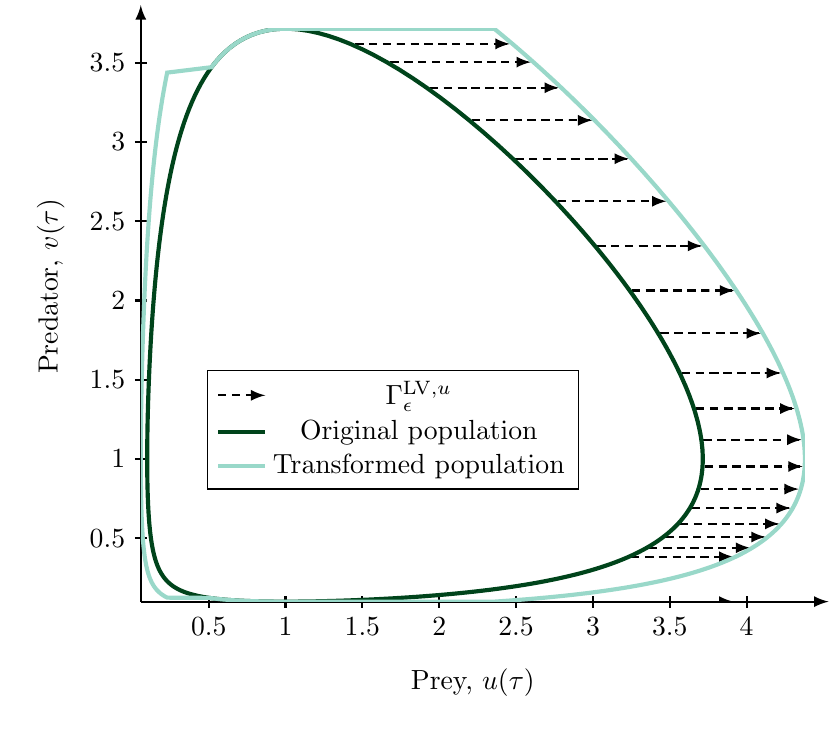
\begin{tikzpicture}
  % The axis of the plot
\begin{axis}[
    xlabel={Prey, $u(\tau)$},
    ylabel={Predator, $v(\tau)$},
    x label style={at={(axis description cs:0.5,-0.1)},anchor=north},
    y label style={at={(axis description cs:-0.1,0.55)},rotate=90,anchor=south},
    scaled x ticks = false,
    legend style={at={(axis description cs:0.1,0.3)},anchor=west,nodes={scale=1.00, transform shape}},    
    grid style=dashed,
]
\addplot[
color=black,->,>=latex,densely dashed
]
coordinates {%
(3.2334201912020424,nan)
(3.2478831891995816,0.1)
(3.2623175920734555,0.1)
(3.2767238190285175,0.10000000000000002)
(3.2911022794843294,0.1)
(3.3054533733887426,0.1)
(3.3197774915188134,0.10000000000000002)
(3.3340750157695593,0.1)
(3.3483463194311915,0.1)
(3.362591767455351,0.1)
(3.376811716710895,0.1)
(3.3910065162297274,0.1)
(3.4051765074431297,0.10000000000000002)
(3.41932202440905,0.1)
(3.4334433940307663,0.1)
(3.447540936267309,0.1)
(3.4616149643360337,0.1)
(3.4756657849076866,0.1)
(3.489693698294309,0.1)
(3.503698998630285,0.1)
(3.5176819740467162,0.1)
(3.531642906840164,0.1)
(3.5455820736342294,0.1)
(3.5594997455364976,0.1)
(3.5733961882894945,0.10000000000000002)
(3.587271662416466,0.1)
(3.601126423362151,0.1)
(3.614960721628713,0.1)
(3.6287748029070594,0.1)
(3.6425689082037285,0.1)
(3.656343273963527,0.1)
(3.670098132188087,0.1)
(3.683833710550509,0.1)
(3.697550232506252,0.1)
(3.7112479174004074,0.1)
(3.724926980571516,0.1)
(3.7385876334520467,0.1)
(3.7522300836656797,0.1)
(3.7658545351215054,0.1)
(3.7794611881052704,0.1)
(3.7930502393677714,0.1)
(3.806621882210514,0.10000000000000002)
(3.820176306568726,0.1)
(3.833713699091844,0.09999999999999999)
(3.8472342432215454,0.1)
(3.860738119267432,0.1)
(3.87422550448044,0.1)
(3.887696573124071,0.1)
(3.901151496543504,0.10000000000000002)
(3.9145904432326897,0.1)
};
\addlegendentry{$\Gamma^{\mathrm{LV},u}_{\epsilon}$}
\addplot[
forget plot,
color=black,->,>=latex,densely dashed
]
coordinates {%
(3.2334201912020424,nan)
(3.2478831891995816,0.38300998606608794)
(3.2623175920734555,0.38300998606608794)
(3.2767238190285175,0.383009986066088)
(3.2911022794843294,0.38300998606608794)
(3.3054533733887426,0.38300998606608794)
(3.3197774915188134,0.383009986066088)
(3.3340750157695593,0.38300998606608794)
(3.3483463194311915,0.38300998606608794)
(3.362591767455351,0.38300998606608794)
(3.376811716710895,0.38300998606608794)
(3.3910065162297274,0.3830099860660879)
(3.4051765074431297,0.383009986066088)
(3.41932202440905,0.38300998606608794)
(3.4334433940307663,0.38300998606608794)
(3.447540936267309,0.38300998606608794)
(3.4616149643360337,0.38300998606608794)
(3.4756657849076866,0.38300998606608794)
(3.489693698294309,0.38300998606608794)
(3.503698998630285,0.38300998606608794)
(3.5176819740467162,0.38300998606608794)
(3.531642906840164,0.38300998606608794)
(3.5455820736342294,0.3830099860660879)
(3.5594997455364976,0.38300998606608794)
(3.5733961882894945,0.383009986066088)
(3.587271662416466,0.38300998606608794)
(3.601126423362151,0.38300998606608794)
(3.614960721628713,0.38300998606608794)
(3.6287748029070594,0.38300998606608794)
(3.6425689082037285,0.38300998606608794)
(3.656343273963527,0.38300998606608794)
(3.670098132188087,0.38300998606608794)
(3.683833710550509,0.38300998606608794)
(3.697550232506252,0.38300998606608794)
(3.7112479174004074,0.38300998606608794)
(3.724926980571516,0.38300998606608794)
(3.7385876334520467,0.38300998606608794)
(3.7522300836656797,0.38300998606608794)
(3.7658545351215054,0.38300998606608794)
(3.7794611881052704,0.38300998606608794)
(3.7930502393677714,0.38300998606608794)
(3.806621882210514,0.38300998606608794)
(3.820176306568726,0.38300998606608794)
(3.833713699091844,0.383009986066088)
(3.8472342432215454,0.3830099860660879)
(3.860738119267432,0.38300998606608794)
(3.87422550448044,0.38300998606608794)
(3.887696573124071,0.38300998606608794)
(3.901151496543504,0.383009986066088)
(3.9145904432326897,0.38300998606608794)
};
\addplot[
forget plot,
color=black,->,>=latex,densely dashed
]
coordinates {%
(3.350086888283124,nan)
(3.3643292042619737,0.4396052502340176)
(3.3785460644998095,0.4396052502340176)
(3.3927378170880833,0.4396052502340176)
(3.4069048025458932,0.4396052502340176)
(3.42104735404614,0.4396052502340176)
(3.4351657976331804,0.4396052502340176)
(3.449260452432268,0.4396052502340176)
(3.46333163085119,0.4396052502340176)
(3.4773796387744462,0.4396052502340176)
(3.4914047757502895,0.4396052502340176)
(3.5054073351709722,0.4396052502340176)
(3.5193876044464694,0.4396052502340176)
(3.533345865171981,0.43960525023401764)
(3.547282393289481,0.4396052502340176)
(3.5611974592435622,0.4396052502340176)
(3.5750913281318315,0.4396052502340176)
(3.588964259850069,0.4396052502340176)
(3.6028165092323965,0.4396052502340176)
(3.6166483261866373,0.4396052502340176)
(3.6304599558250863,0.4396052502340176)
(3.644251638590863,0.43960525023401764)
(3.6580236103799084,0.4396052502340176)
(3.6717761026595563,0.4396052502340176)
(3.6855093425820193,0.4396052502340176)
(3.6992235530952513,0.4396052502340176)
(3.7129189530497,0.43960525023401764)
(3.7265957573017046,0.4396052502340176)
(3.740254176813578,0.4396052502340176)
(3.753894418750506,0.4396052502340176)
(3.767516686574385,0.4396052502340176)
(3.7811211801347056,0.4396052502340176)
(3.7947080957566137,0.4396052502340176)
(3.8082776263262366,0.4396052502340176)
(3.8218299613733846,0.4396052502340176)
(3.8353652871517347,0.4396052502340176)
(3.848883786716567,0.4396052502340176)
(3.862385640000168,0.43960525023401764)
(3.8758710238849723,0.4396052502340176)
(3.889340112274528,0.4396052502340176)
(3.90279307616236,0.4396052502340176)
(3.916230083698819,0.43960525023401753)
(3.9296513002559705,0.43960525023401764)
(3.94305688849061,0.4396052502340176)
(3.9564470084054553,0.4396052502340176)
(3.969821817408592,0.4396052502340176)
(3.9831814703712194,0.4396052502340176)
(3.9965261196837782,0.43960525023401764)
(4.009855915310482,0.4396052502340176)
(4.023171004842337,0.4396052502340176)
};
\addplot[
forget plot,
color=black,->,>=latex,densely dashed
]
coordinates {%
(3.457986883991823,nan)
(3.472043661809039,0.5079897885210969)
(3.4860774555758667,0.5079897885210969)
(3.5000885610032006,0.5079897885210969)
(3.514077267754414,0.5079897885210969)
(3.528043859615157,0.5079897885210969)
(3.5419886146571447,0.5079897885210969)
(3.555911805396142,0.5079897885210969)
(3.5698136989443987,0.5079897885210969)
(3.5836945571577754,0.5079897885210969)
(3.5975546367777818,0.5079897885210969)
(3.6113941895687396,0.5079897885210969)
(3.625213462450275,0.5079897885210969)
(3.6390126976253265,0.5079897885210969)
(3.6527921327038677,0.5079897885210969)
(3.6665520008224934,0.5079897885210969)
(3.6802925307600654,0.5079897885210969)
(3.694013947049548,0.5079897885210969)
(3.7077164700862077,0.5079897885210969)
(3.7214003162323044,0.5079897885210969)
(3.73506569791842,0.5079897885210969)
(3.7487128237415517,0.5079897885210969)
(3.7623418985601016,0.5079897885210969)
(3.7759531235858637,0.5079897885210969)
(3.789546696473009,0.5079897885210969)
(3.8031228114049567,0.5079897885210969)
(3.8166816591773394,0.5079897885210969)
(3.83022342727958,0.5079897885210969)
(3.8437482999734414,0.5079897885210969)
(3.8572564583693114,0.5079897885210969)
(3.8707480805001873,0.5079897885210969)
(3.8842233413934646,0.5079897885210969)
(3.8976824131405845,0.5079897885210969)
(3.9111254649646483,0.5079897885210969)
(3.9245526632860317,0.5079897885210969)
(3.9379641717861142,0.5079897885210969)
(3.9513601514691494,0.5079897885210969)
(3.964740760722372,0.5079897885210969)
(3.978106155374381,0.5079897885210969)
(3.9914564887518744,0.5079897885210969)
(4.00479191173478,0.5079897885210969)
(4.018112572809849,0.5079897885210969)
(4.03141861812275,0.5079897885210969)
(4.044710191528729,0.5079897885210969)
(4.057987434641875,0.5079897885210969)
(4.071250486883031,0.5079897885210969)
(4.084499485526417,0.5079897885210969)
(4.097734565744984,0.5079897885210969)
(4.1109558606545535,0.5079897885210969)
(4.124163501356778,0.5079897885210969)
};
\addplot[
forget plot,
color=black,->,>=latex,densely dashed
]
coordinates {%
(3.553242540113277,nan)
(3.56714849870272,0.5906205271026429)
(3.5810333721255083,0.5906205271026429)
(3.5948974180934568,0.5906205271026429)
(3.608740889315269,0.5906205271026429)
(3.622564033629882,0.5906205271026429)
(3.636367094135333,0.5906205271026429)
(3.650150309313278,0.5906205271026429)
(3.663913913149373,0.5906205271026429)
(3.677658135249647,0.5906205271026429)
(3.691383200953072,0.5906205271026429)
(3.7050893314404365,0.5906205271026429)
(3.718776743839708,0.5906205271026429)
(3.7324456513279904,0.5906205271026429)
(3.7460962632302306,0.5906205271026429)
(3.759728785114791,0.5906205271026429)
(3.773343418886011,0.5906205271026429)
(3.786940362873865,0.5906205271026429)
(3.8005198119208434,0.5906205271026429)
(3.814081957466139,0.5906205271026429)
(3.827626987627263,0.5906205271026429)
(3.841155087279166,0.5906205271026429)
(3.8546664381309688,0.5906205271026429)
(3.868161218800382,0.5906205271026429)
(3.8816396048859114,0.5906205271026429)
(3.8951017690369083,0.5906205271026429)
(3.9085478810214176,0.5906205271026429)
(3.9219781077927345,0.5906205271026429)
(3.9353926135526995,0.5906205271026429)
(3.948791559814412,0.5906205271026429)
(3.9621751054625602,0.5906205271026429)
(3.9755434068121267,0.5906205271026429)
(3.9888966176654312,0.5906205271026429)
(4.002234889367574,0.5906205271026429)
(4.015558370860309,0.5906205271026429)
(4.028867208734435,0.5906205271026429)
(4.042161547280712,0.5906205271026429)
(4.055441528539402,0.5906205271026429)
(4.068707292348431,0.5906205271026429)
(4.081958976390258,0.5906205271026429)
(4.095196716237468,0.5906205271026429)
(4.108420645397142,0.5906205271026429)
(4.121630895354037,0.5906205271026429)
(4.134827595612629,0.5906205271026429)
(4.1480108737380315,0.5906205271026429)
(4.161180855395855,0.5906205271026429)
(4.17433766439101,0.5906205271026429)
(4.187481422705515,0.5906205271026429)
(4.200612250535317,0.5906205271026429)
(4.213730266326185,0.5906205271026429)
};
\addplot[
forget plot,
color=black,->,>=latex,densely dashed
]
coordinates {%
(3.6312219325940935,nan)
(3.6450125209769855,0.6902947366797437)
(3.658783411277366,0.6902947366797437)
(3.67253483472116,0.6902947366797437)
(3.6862670182257062,0.6902947366797437)
(3.6999801845099762,0.6902947366797437)
(3.713674552201232,0.6902947366797437)
(3.7273503359382367,0.6902947366797437)
(3.7410077464711593,0.6902947366797437)
(3.754646990758303,0.6902947366797437)
(3.768268272059773,0.6902947366797437)
(3.7818717900282044,0.6902947366797437)
(3.7954577407966705,0.6902947366797437)
(3.8090263170638563,0.6902947366797437)
(3.8225777081766266,0.6902947366797437)
(3.83611210021006,0.6902947366797437)
(3.849629676045071,0.6902947366797437)
(3.863130615443669,0.6902947366797437)
(3.8766150951219904,0.6902947366797437)
(3.8900832888211383,0.6902947366797437)
(3.903535367375939,0.6902947366797437)
(3.9169714987816735,0.6902947366797437)
(3.93039184825887,0.6902947366797437)
(3.943796578316206,0.6902947366797437)
(3.9571858488116143,0.6902947366797437)
(3.9705598170116247,0.6902947366797437)
(3.9839186376490234,0.6902947366797437)
(3.9972624629788855,0.6902947366797437)
(4.010591442832856,0.6902947366797437)
(4.023905724672731,0.6902947366797437)
(4.037205453641009,0.6902947366797437)
(4.050490772611514,0.6902947366797437)
(4.063761822237929,0.6902947366797437)
(4.0770187410011385,0.6902947366797437)
(4.090261665255299,0.6902947366797437)
(4.1034907292726555,0.6902947366797437)
(4.116706065287163,0.6902947366797437)
(4.1299078035369465,0.6902947366797437)
(4.143096072305641,0.6902947366797437)
(4.1562709979626336,0.6902947366797437)
(4.16943270500226,0.6902947366797437)
(4.182581316081984,0.6902947366797437)
(4.195716952059575,0.6902947366797437)
(4.208839732029348,0.6902947366797437)
(4.221949773357464,0.6902947366797437)
(4.235047191716331,0.6902947366797437)
(4.248132101118145,0.6902947366797437)
(4.261204613947579,0.6902947366797437)
(4.274264840993656,0.6902947366797437)
(4.2873128914808225,0.6902947366797436)
};
\addplot[
forget plot,
color=black,->,>=latex,densely dashed
]
coordinates {%
(3.686572798684044,nan)
(3.700285543707692,0.8100532332062869)
(3.7139794949642546,0.8100532332062869)
(3.7276548670047602,0.8100532332062867)
(3.7413118704938433,0.8100532332062869)
(3.75495071230639,0.8100532332062869)
(3.7685715956211414,0.8100532332062867)
(3.782174720011359,0.8100532332062869)
(3.7957602815326674,0.8100532332062869)
(3.8093284728081724,0.8100532332062869)
(3.82287948311097,0.8100532332062869)
(3.8364134984441263,0.8100532332062869)
(3.8499307016182436,0.8100532332062867)
(3.863431272326673,0.8100532332062869)
(3.8769153872184945,0.8100532332062869)
(3.890383219969306,0.8100532332062869)
(3.9038349413499414,0.8100532332062869)
(3.917270719293151,0.8100532332062869)
(3.9306907189583553,0.8100532332062869)
(3.9440951027945075,0.8100532332062869)
(3.9574840306011527,0.8100532332062869)
(3.9708576595877374,0.8100532332062869)
(3.984216144431234,0.8100532332062869)
(3.9975596373321296,0.8100532332062869)
(4.010888288068854,0.8100532332062867)
(4.024202244050674,0.8100532332062869)
(4.037501650369127,0.8100532332062869)
(4.050786649848044,0.8100532332062869)
(4.064057383092177,0.8100532332062869)
(4.077313988534357,0.8100532332062869)
(4.09055660248216,0.8100532332062869)
(4.103785359161806,0.8100532332062869)
(4.11700039076232,0.8100532332062869)
(4.13020182747783,0.8100532332062869)
(4.143389797548877,0.8100532332062869)
(4.156564427302643,0.8100532332062869)
(4.169725841192124,0.8100532332062869)
(4.182874161834275,0.8100532332062869)
(4.196009510047181,0.8100532332062869)
(4.209132004886267,0.8100532332062869)
(4.222241763679578,0.8100532332062869)
(4.235338902062167,0.8100532332062867)
(4.248423534009611,0.8100532332062869)
(4.261495771870681,0.810053233206287)
(4.274555726399198,0.8100532332062869)
(4.2876035067851,0.8100532332062869)
(4.300639220684726,0.8100532332062869)
(4.3136629742503745,0.8100532332062869)
(4.326674872159121,0.8100532332062867)
(4.33967501764094,0.8100532332062869)
};
\addplot[
forget plot,
color=black,->,>=latex,densely dashed
]
coordinates {%
(3.7133864264845857,nan)
(3.7270625992984576,0.9529683465757389)
(3.7407203945105802,0.9529683465757389)
(3.7543600191581024,0.9529683465757389)
(3.767981676578051,0.9529683465757389)
(3.7815855664980953,0.9529683465757388)
(3.7951718851245206,0.9529683465757389)
(3.80874082522746,0.9529683465757389)
(3.822292576223512,0.9529683465757389)
(3.8358273242558316,0.9529683465757388)
(3.8493452522717972,0.9529683465757388)
(3.8628465400983245,0.9529683465757389)
(3.8763313645149378,0.9529683465757389)
(3.889799899324659,0.9529683465757389)
(3.9032523154228103,0.9529683465757389)
(3.9166887808637783,0.9529683465757389)
(3.9301094609258556,0.9529683465757389)
(3.94351451817418,0.9529683465757389)
(3.956904112521873,0.9529683465757388)
(3.9702784012894203,0.9529683465757389)
(3.9836375392623733,0.9529683465757388)
(3.996981678747402,0.9529683465757389)
(4.0103109696267945,0.9529683465757389)
(4.023625559411411,0.9529683465757389)
(4.036925593292191,0.9529683465757389)
(4.050211214190214,0.9529683465757389)
(4.063482562805416,0.9529683465757389)
(4.076739777663952,0.9529683465757389)
(4.089982995164284,0.9529683465757389)
(4.103212349621888,0.9529683465757389)
(4.116427973313452,0.9529683465757389)
(4.1296299965185765,0.9529683465757389)
(4.142818547561623,0.9529683465757389)
(4.155993752851875,0.9529683465757389)
(4.1691557369227485,0.9529683465757389)
(4.182304622469992,0.9529683465757389)
(4.1954405303888915,0.9529683465757388)
(4.208563579810521,0.952968346575739)
(4.221673888137066,0.9529683465757389)
(4.23477157107625,0.9529683465757389)
(4.2478567426748794,0.9529683465757388)
(4.260929515351562,0.952968346575739)
(4.273989999928592,0.9529683465757389)
(4.287038305663044,0.9529683465757389)
(4.300074540277104,0.9529683465757389)
(4.313098809987648,0.952968346575739)
(4.3261112195350915,0.9529683465757389)
(4.339111872211554,0.9529683465757389)
(4.3521008698883135,0.9529683465757389)
(4.3650783130426305,0.9529683465757388)
};
\addplot[
forget plot,
color=black,->,>=latex,densely dashed
]
coordinates {%
(3.7055547526917274,nan)
(3.7192415327943085,1.1217713684816235)
(3.7329098151617055,1.1217713684816235)
(3.74655980898965,1.1217713684816235)
(3.760191719720499,1.1217713684816235)
(3.7738057491356725,1.1217713684816235)
(3.7874020954452257,1.1217713684816235)
(3.8009809533746335,1.1217713684816235)
(3.814542514248889,1.1217713684816235)
(3.8280869660740313,1.1217713684816235)
(3.8416144936161856,1.1217713684816235)
(3.8551252784782113,1.1217713684816235)
(3.8686194991740535,1.1217713684816235)
(3.8820973312008586,1.1217713684816235)
(3.895558947108971,1.1217713684816235)
(3.90900451656985,1.1217713684816235)
(3.9224342064420035,1.1217713684816235)
(3.935848180835006,1.1217713684816235)
(3.9492466011716614,1.1217713684816235)
(3.9626296262483787,1.1217713684816235)
(3.975997412293832,1.1217713684816235)
(3.98935011302594,1.1217713684816235)
(4.00268787970726,1.1217713684816235)
(4.016010861198807,1.1217713684816235)
(4.029319204012391,1.1217713684816235)
(4.042613052361498,1.1217713684816235)
(4.055892548210764,1.1217713684816235)
(4.069157831324112,1.1217713684816235)
(4.082409039311564,1.1217713684816235)
(4.095646307674642,1.1217713684816233)
(4.108869769851269,1.1217713684816235)
(4.12207955725811,1.1217713684816235)
(4.135275799333071,1.1217713684816235)
(4.148458623576071,1.1217713684816235)
(4.1616281555888595,1.1217713684816235)
(4.174784519113789,1.1217713684816235)
(4.187927836071583,1.1217713684816235)
(4.201058226598137,1.1217713684816235)
(4.214175809080361,1.1217713684816235)
(4.227280700191116,1.1217713684816235)
(4.2403730149232635,1.1217713684816235)
(4.253452866622854,1.1217713684816235)
(4.266520367021479,1.1217713684816235)
(4.279575626267824,1.1217713684816235)
(4.292618752958424,1.1217713684816235)
(4.305649854167677,1.1217713684816235)
(4.318669035477102,1.1217713684816235)
(4.3316764010039,1.1217713684816235)
(4.344672053428802,1.1217713684816235)
(4.3576560940232625,1.1217713684816235)
};
\addplot[
forget plot,
color=black,->,>=latex,densely dashed
]
coordinates {%
(3.657375838918677,nan)
(3.6711292429195903,1.318288435930125)
(3.6848633839670066,1.318288435930125)
(3.6985784852043357,1.318288435930125)
(3.7122747656725408,1.318288435930125)
(3.725952440413683,1.318288435930125)
(3.7396117205711596,1.318288435930125)
(3.7532528134867498,1.318288435930125)
(3.7668759227945925,1.318288435930125)
(3.7804812485122077,1.318288435930125)
(3.7940689871286897,1.318288435930125)
(3.807639331690154,1.318288435930125)
(3.8211924718825694,1.318288435930125)
(3.8347285941120477,1.318288435930125)
(3.8482478815827,1.318288435930125)
(3.861750514372147,1.318288435930125)
(3.8752366695047646,1.318288435930125)
(3.888706521022746,1.318288435930125)
(3.9021602400550717,1.318288435930125)
(3.9155979948844406,1.318288435930125)
(3.9290199510122594,1.318288435930125)
(3.942426271221737,1.318288435930125)
(3.955817115639167,1.318288435930125)
(3.9691926417934456,1.318288435930125)
(3.9825530046739117,1.318288435930125)
(3.995898356786531,1.318288435930125)
(4.0092288482085126,1.318288435930125)
(4.0225446266414,1.318288435930125)
(4.035845837462524,1.318288435930125)
(4.049132623775766,1.318288435930125)
(4.062405126459569,1.318288435930125)
(4.075663484214914,1.318288435930125)
(4.088907833611397,1.318288435930125)
(4.102138309132175,1.318288435930125)
(4.115355043217709,1.318288435930125)
(4.12855816630834,1.318288435930125)
(4.141747806885739,1.318288435930125)
(4.154924091513263,1.318288435930125)
(4.1680871448752566,1.318288435930125)
(4.1812370898153315,1.318288435930125)
(4.194374047373651,1.318288435930125)
(4.207498136823256,1.318288435930125)
(4.220609475705467,1.318288435930125)
(4.233708179864373,1.318288435930125)
(4.246794363480461,1.318288435930125)
(4.259868139103387,1.318288435930125)
(4.272929617683933,1.318288435930125)
(4.285978908605169,1.318288435930125)
(4.299016119712837,1.318288435930125)
(4.312041357344997,1.3182884359301252)
};
\addplot[
forget plot,
color=black,->,>=latex,densely dashed
]
coordinates {%
(3.564419247258668,nan)
(3.578308240999011,1.5427003192699082)
(3.5921763570728267,1.5427003192699082)
(3.6060238491606706,1.5427003192699082)
(3.6198509660475273,1.5427003192699082)
(3.6336579517525145,1.5427003192699082)
(3.6474450456542526,1.5427003192699082)
(3.661212482612034,1.5427003192699082)
(3.674960493082985,1.5427003192699082)
(3.688689303235357,1.5427003192699082)
(3.7023991350581227,1.5427003192699082)
(3.716090206467011,1.5427003192699082)
(3.7297627314071287,1.5427003192699082)
(3.7434169199522898,1.5427003192699082)
(3.7570529784011977,1.5427003192699082)
(3.7706711093705856,1.5427003192699082)
(3.7842715118854406,1.5427003192699082)
(3.797854381466413,1.5427003192699082)
(3.8114199102145374,1.5427003192699082)
(3.8249682868933297,1.5427003192699082)
(3.8384996970084035,1.5427003192699082)
(3.8520143228846573,1.5427003192699085)
(3.865512343741142,1.5427003192699082)
(3.8789939357636967,1.542700319269908)
(3.8924592721754134,1.5427003192699082)
(3.905908523305036,1.5427003192699085)
(3.9193418566531935,1.5427003192699082)
(3.9327594369573937,1.542700319269908)
(3.9461614262538545,1.5427003192699082)
(3.9595479839387586,1.5427003192699085)
(3.972919266827184,1.5427003192699082)
(3.9862754292104796,1.542700319269908)
(3.9996166229120056,1.5427003192699082)
(4.0129429973413195,1.5427003192699082)
(4.026254699546845,1.5427003192699082)
(4.039551874267088,1.5427003192699082)
(4.052834663980429,1.5427003192699082)
(4.066103208953562,1.5427003192699082)
(4.079357647288611,1.5427003192699082)
(4.092598114968972,1.5427003192699082)
(4.105824745903911,1.5427003192699082)
(4.119037671971991,1.5427003192699082)
(4.132237023063319,1.5427003192699085)
(4.145422927120695,1.5427003192699082)
(4.1585955101796666,1.5427003192699082)
(4.1717548964075455,1.5427003192699082)
(4.184901208141401,1.542700319269908)
(4.19803456592508,1.5427003192699082)
(4.21115508854527,1.5427003192699082)
(4.224262893066643,1.5427003192699082)
};
\addplot[
forget plot,
color=black,->,>=latex,densely dashed
]
coordinates {%
(3.424569728349855,nan)
(3.438682211114166,1.7927295166218755)
(3.452770983603654,1.7927295166218755)
(3.4668363565817564,1.7927295166218755)
(3.4808786343359377,1.7927295166218755)
(3.494898114862977,1.7927295166218755)
(3.508895090047563,1.7927295166218755)
(3.522869845834443,1.7927295166218755)
(3.5368226623944143,1.7927295166218755)
(3.5507538142844286,1.7927295166218755)
(3.564663570602057,1.7927295166218755)
(3.578552195134554,1.7927295166218755)
(3.5924199465027598,1.7927295166218755)
(3.60626707830004,1.7927295166218755)
(3.620093839226495,1.7927295166218755)
(3.6339004732186013,1.7927295166218755)
(3.647687219574505,1.7927295166218755)
(3.661454313075117,1.7927295166218755)
(3.6752019841012076,1.7927295166218755)
(3.6889304587466274,1.7927295166218755)
(3.702639958927847,1.7927295166218755)
(3.7163307024899237,1.7927295166218755)
(3.730002903309067,1.7927295166218755)
(3.743656771391912,1.7927295166218755)
(3.757292512971477,1.7927295166218755)
(3.7709103306008744,1.7927295166218755)
(3.7845104232426188,1.7927295166218755)
(3.7980929863565276,1.7927295166218755)
(3.8116582119842644,1.7927295166218755)
(3.8252062888313985,1.7927295166218755)
(3.838737402346972,1.7927295166218755)
(3.8522517348006478,1.7927295166218755)
(3.865749465357539,1.7927295166218755)
(3.879230770150801,1.7927295166218755)
(3.892695822352064,1.7927295166218755)
(3.9061447922397923,1.7927295166218755)
(3.9195778472656295,1.7927295166218755)
(3.932995152118826,1.7927295166218755)
(3.9463968687887796,1.7927295166218755)
(3.9597831566257984,1.7927295166218755)
(3.973154172400107,1.7927295166218755)
(3.9865100703591967,1.7927295166218755)
(3.999851002283531,1.7927295166218755)
(4.013177117540716,1.7927295166218755)
(4.026488563138132,1.7927295166218755)
(4.039785483774131,1.7927295166218755)
(4.0530680218878015,1.7927295166218755)
(4.066336317707387,1.7927295166218755)
(4.079590509297374,1.7927295166218755)
(4.092830732604318,1.7927295166218755)
};
\addplot[
forget plot,
color=black,->,>=latex,densely dashed
]
coordinates {%
(3.2390353870850834,nan)
(3.2534872395072365,2.062971818697081)
(3.2679106606433708,2.062971818697081)
(3.282306065863454,2.062971818697081)
(3.2966738608754214,2.062971818697081)
(3.311014442033726,2.062971818697081)
(3.325328196635477,2.062971818697081)
(3.3396155032046497,2.062971818697081)
(3.3538767317649887,2.062971818697081)
(3.3681122441021314,2.062971818697081)
(3.3823223940154716,2.062971818697081)
(3.396507527560249,2.062971818697081)
(3.410667983280323,2.062971818697081)
(3.424804092432064,2.062971818697081)
(3.4389161791997767,2.062971818697081)
(3.453004560903026,2.062971818697081)
(3.4670695481962697,2.062971818697081)
(3.4811114452610887,2.062971818697081)
(3.495130549991409,2.062971818697081)
(3.509127154171972,2.062971818697081)
(3.5231015436502466,2.062971818697081)
(3.5370539985028073,2.062971818697081)
(3.550984793194681,2.062971818697081)
(3.56489419673412,2.062971818697081)
(3.5787824728214943,2.062971818697081)
(3.5926498799931004,2.062971818697081)
(3.606496671760032,2.062971818697081)
(3.620323096742296,2.062971818697081)
(3.634129398798396,2.062971818697081)
(3.647915817150547,2.062971818697081)
(3.6616825865057026,2.062971818697081)
(3.675429937172586,2.062971818697081)
(3.6891580951748484,2.062971818697081)
(3.7028672823605477,2.062971818697081)
(3.716557716508057,2.062971818697081)
(3.7302296114285753,2.062971818697081)
(3.7438831770653476,2.062971818697081)
(3.757518619589741,2.062971818697081)
(3.771136141494281,2.062971818697081)
(3.784735941682781,2.062971818697081)
(3.798318215557657,2.062971818697081)
(3.8118831551045553,2.062971818697081)
(3.825430948974366,2.062971818697081)
(3.8389617825627536,2.062971818697081)
(3.8524758380872615,2.062971818697081)
(3.8659732946621093,2.062971818697081)
(3.879454328370741,2.062971818697081)
(3.8929191123362292,2.062971818697081)
(3.906367816789596,2.062971818697081)
(3.9198006091361304,2.062971818697081)
};
\addplot[
forget plot,
color=black,->,>=latex,densely dashed
]
coordinates {%
(3.0129868711372794,nan)
(3.0279362503837044,2.3446765493846122)
(3.0428493217409933,2.3446765493846122)
(3.057726699670682,2.3446765493846122)
(3.07256898205046,2.3446765493846122)
(3.0873767507884353,2.3446765493846122)
(3.10215057240874,2.3446765493846122)
(3.1168909986098683,2.3446765493846122)
(3.131598566797329,2.3446765493846122)
(3.1462738005920214,2.3446765493846122)
(3.1609172103156795,2.3446765493846122)
(3.1755292934546357,2.3446765493846122)
(3.1901105351030696,2.3446765493846122)
(3.204661408386838,2.3446765493846122)
(3.21918237486892,2.3446765493846122)
(3.2336738849374376,2.344676549384612)
(3.248136378177148,2.3446765493846122)
(3.262570283725105,2.3446765493846122)
(3.2769760206122203,2.3446765493846122)
(3.291353998089287,2.3446765493846122)
(3.305704615940899,2.3446765493846122)
(3.320028264786012,2.3446765493846122)
(3.3343253263665047,2.3446765493846122)
(3.348596173824203,2.3446765493846122)
(3.362841171966937,2.3446765493846122)
(3.3770606775241423,2.3446765493846122)
(3.391255039392525,2.3446765493846122)
(3.4054245988722274,2.3446765493846122)
(3.4195696898939634,2.3446765493846122)
(3.433690639237534,2.3446765493846122)
(3.4477877667421066,2.344676549384612)
(3.4618613855086586,2.3446765493846122)
(3.4759118020949105,2.3446765493846122)
(3.4899393167031056,2.3446765493846122)
(3.5039442233609464,2.3446765493846122)
(3.5179268100959917,2.3446765493846122)
(3.531887359103792,2.3446765493846122)
(3.5458261469100507,2.3446765493846122)
(3.559743444527056,2.3446765493846122)
(3.5736395176046294,2.3446765493846122)
(3.587514626575827,2.3446765493846122)
(3.601369026797619,2.3446765493846122)
(3.6152029686867384,2.3446765493846122)
(3.629016697850929,2.3446765493846122)
(3.6428104552157445,2.3446765493846122)
(3.6565844771471245,2.3446765493846122)
(3.670338995569871,2.3446765493846122)
(3.6840742380822338,2.3446765493846122)
(3.6977904280667273,2.3446765493846122)
(3.711487784797353,2.3446765493846122)
};
\addplot[
forget plot,
color=black,->,>=latex,densely dashed
]
coordinates {%
(2.7554824208200257,nan)
(2.771153571470712,2.626251840284192)
(2.7867748431596957,2.626251840284192)
(2.8023472589268548,2.626251840284192)
(2.817871808297612,2.626251840284192)
(2.833349448788742,2.626251840284192)
(2.8487811073285387,2.626251840284192)
(2.864167681597216,2.626251840284192)
(2.8795100412929355,2.626251840284192)
(2.894809029328441,2.626251840284192)
(2.910065462962889,2.626251840284192)
(2.9252801348731006,2.626251840284192)
(2.9404538141681527,2.626251840284192)
(2.955587247350762,2.6262518402841915)
(2.970681159229643,2.626251840284192)
(2.9857362537840713,2.626251840284192)
(3.000753214985789,2.626251840284192)
(3.0157327075793594,2.626251840284192)
(3.0306753778240307,2.626251840284192)
(3.0455818541993165,2.626251840284192)
(3.0604527480764383,2.626251840284192)
(3.075288654357619,2.626251840284192)
(3.0900901520850934,2.626251840284192)
(3.104857805021563,2.626251840284192)
(3.119592162203713,2.626251840284192)
(3.1342937584703003,2.626251840284192)
(3.1489631149662287,2.6262518402841915)
(3.1636007396239205,2.626251840284192)
(3.1782071276232333,2.626251840284192)
(3.192782761831064,2.626251840284192)
(3.20732811322173,2.626251840284192)
(3.2218436412791482,2.626251840284192)
(3.2363297943817506,2.626251840284192)
(3.250787010171051,2.626251840284192)
(3.2652157159046817,2.626251840284192)
(3.279616328794708,2.626251840284192)
(3.293989256331951,2.626251840284192)
(3.308334896597029,2.626251840284192)
(3.322653638558758,2.626251840284192)
(3.3369458623605586,2.626251840284192)
(3.35121193959542,2.626251840284192)
(3.3654522335700072,2.626251840284192)
(3.379667099558398,2.626251840284192)
(3.393856885045974,2.626251840284192)
(3.40802192996389,2.626251840284192)
(3.4221625669146083,2.626251840284192)
(3.4362791213888637,2.626251840284192)
(3.450371911974483,2.626251840284192)
(3.4644412505574227,2.626251840284192)
(3.4784874425153642,2.626251840284192)
};
\addplot[
forget plot,
color=black,->,>=latex,densely dashed
]
coordinates {%
(2.4785073974533534,nan)
(2.495232976548041,2.894569606620069)
(2.511883906172174,2.894569606620069)
(2.5284621440553328,2.894569606620069)
(2.544969565853838,2.894569606620069)
(2.5614079698598884,2.894569606620069)
(2.577779081369657,2.894569606620069)
(2.5940845567400204,2.894569606620069)
(2.6103259871606035,2.894569606620069)
(2.6265049021651543,2.894569606620069)
(2.6426227729036706,2.894569606620069)
(2.658681015196036,2.894569606620069)
(2.674680992382313,2.894569606620069)
(2.6906240179887293,2.894569606620069)
(2.7065113582218934,2.894569606620069)
(2.7223442343052113,2.894569606620069)
(2.738123824669422,2.894569606620069)
(2.7538512670082085,2.894569606620069)
(2.76952766020891,2.894569606620069)
(2.785154066167459,2.894569606620069)
(2.8007315114959246,2.894569606620069)
(2.816260989130298,2.894569606620069)
(2.831743459845558,2.894569606620069)
(2.8471798536844597,2.8945696066200695)
(2.8625710713059562,2.894569606620069)
(2.877917985258719,2.894569606620069)
(2.893221441184763,2.894569606620069)
(2.9084822589578057,2.894569606620069)
(2.923701233760624,2.894569606620069)
(2.938879137105363,2.8945696066200695)
(2.954016717800423,2.894569606620069)
(2.969114702867318,2.894569606620069)
(2.984173798410614,2.894569606620069)
(2.999194690443853,2.894569606620069)
(3.0141780456741474,2.894569606620069)
(3.0291245122479418,2.894569606620069)
(3.0440347204602594,2.894569606620069)
(3.058909283429597,2.894569606620069)
(3.0737487977404707,2.894569606620069)
(3.0885538440554896,2.894569606620069)
(3.1033249876987,2.894569606620069)
(3.11806277921183,2.894569606620069)
(3.132767754884951,2.894569606620069)
(3.1474404372629867,2.894569606620069)
(3.1620813356293844,2.894569606620069)
(3.1766909464682045,2.894569606620069)
(3.1912697539057824,2.8945696066200695)
(3.2058182301330644,2.894569606620069)
(3.2203368358096247,2.894569606620069)
(3.234826020450338,2.894569606620069)
};
\addplot[
forget plot,
color=black,->,>=latex,densely dashed
]
coordinates {%
(2.1952864569614197,nan)
(2.2135891729814547,3.136819528140607)
(2.231768020117077,3.136819528140607)
(2.249827430244664,3.1368195281406073)
(2.26777158205095,3.136819528140607)
(2.2856044207432333,3.136819528140607)
(2.3033296758327277,3.1368195281406073)
(2.320950877215915,3.136819528140607)
(2.3384713697499997,3.136819528140607)
(2.3558943264887326,3.136819528140607)
(2.373222760728584,3.136819528140607)
(2.3904595369916763,3.1368195281406064)
(2.4076073810584266,3.1368195281406073)
(2.4246688891483403,3.136819528140607)
(2.441646536335658,3.136819528140607)
(2.4585426842762925,3.136819528140607)
(2.4753595883136827,3.136819528140607)
(2.492099404023429,3.136819528140607)
(2.50876419324992,3.136819528140607)
(2.5253559296822745,3.136819528140607)
(2.5418765040118245,3.136819528140607)
(2.558327728708841,3.136819528140607)
(2.5747113424522814,3.1368195281406064)
(2.591029014242843,3.1368195281406064)
(2.6072823472265334,3.1368195281406073)
(2.6234728822532474,3.1368195281406073)
(2.639602101192439,3.136819528140607)
(2.6556714300258255,3.136819528140607)
(2.6716822417351636,3.136819528140607)
(2.6876358590014275,3.136819528140607)
(2.703533556730222,3.136819528140607)
(2.7193765644168812,3.136819528140607)
(2.7351660683635193,3.136819528140607)
(2.7509032137591767,3.136819528140607)
(2.766589106633252,3.136819528140607)
(2.7822248156915137,3.136819528140607)
(2.7978113740431905,3.136819528140607)
(2.8133497808269334,3.136819528140607)
(2.828841002742772,3.136819528140607)
(2.844285975496634,3.136819528140607)
(2.8596856051634174,3.136819528140607)
(2.8750407694741824,3.136819528140607)
(2.8903523190326137,3.136819528140607)
(2.9056210784649554,3.136819528140607)
(2.920847847508999,3.1368195281406064)
(2.936033402044498,3.136819528140607)
(2.951178495069893,3.1368195281406064)
(2.966283857628316,3.136819528140607)
(2.9813501996861063,3.1368195281406073)
(2.996378210966786,3.136819528140607)
};
\addplot[
forget plot,
color=black,->,>=latex,densely dashed
]
coordinates {%
(1.9183432004123362,nan)
(1.9391108430236557,3.3423883774232857)
(1.959644260246242,3.3423883774232857)
(1.9799558496551697,3.3423883774232857)
(2.0000569670111514,3.3423883774232857)
(2.0199580444983867,3.3423883774232857)
(2.0396686922663916,3.3423883774232857)
(2.0591977860692094,3.3423883774232857)
(2.078553543258581,3.3423883774232857)
(2.0977435889676666,3.3423883774232857)
(2.1167750139891153,3.3423883774232857)
(2.1356544255862846,3.342388377423285)
(2.1543879922638496,3.3423883774232857)
(2.1729814833524896,3.3423883774232857)
(2.1914403041230437,3.3423883774232857)
(2.209769527031767,3.3423883774232857)
(2.2279739196049677,3.3423883774232857)
(2.2460579693942053,3.3423883774232857)
(2.264025906369417,3.3423883774232857)
(2.28188172306407,3.3423883774232857)
(2.2996291927419708,3.3423883774232857)
(2.3172718858179553,3.3423883774232857)
(2.3348131847331506,3.342388377423285)
(2.3522562974588164,3.3423883774232857)
(2.3696042697801833,3.3423883774232857)
(2.3868599964917,3.342388377423285)
(2.404026231620481,3.3423883774232857)
(2.421105597777512,3.3423883774232857)
(2.438100594726829,3.3423883774232857)
(2.455013607250718,3.3423883774232857)
(2.47184691238033,3.3423883774232857)
(2.4886026860531554,3.3423883774232857)
(2.5052830092518508,3.3423883774232857)
(2.5218898736729365,3.3423883774232857)
(2.5384251869685803,3.3423883774232857)
(2.5548907776000855,3.3423883774232857)
(2.571288399337631,3.3423883774232857)
(2.587619735437252,3.3423883774232857)
(2.603886402522867,3.3423883774232857)
(2.620089954198413,3.3423883774232857)
(2.6362318844126253,3.3423883774232857)
(2.6523136305968538,3.342388377423285)
(2.6683365765943083,3.3423883774232857)
(2.6843020553974357,3.3423883774232857)
(2.700211351708534,3.342388377423285)
(2.7160657043373506,3.3423883774232857)
(2.7318663084481516,3.3423883774232857)
(2.7476143176676464,3.342388377423285)
(2.763310846064137,3.3423883774232857)
(2.778956970007374,3.3423883774232857)
};
\addplot[
forget plot,
color=black,->,>=latex,densely dashed
]
coordinates {%
(1.6578841746791864,nan)
(1.6828025917185385,3.5042060530796926)
(1.7071917450325043,3.5042060530796926)
(1.7310976877524098,3.504206053079693)
(1.7545602141492835,3.5042060530796926)
(1.77761398747864,3.5042060530796926)
(1.800289419389519,3.504206053079693)
(1.822613364660435,3.5042060530796926)
(1.8446096765463897,3.5042060530796926)
(1.8662996554566045,3.5042060530796926)
(1.887702414976871,3.5042060530796926)
(1.9088351831124626,3.504206053079692)
(1.9297135522315678,3.504206053079693)
(1.950351687994487,3.5042060530796926)
(1.9707625052040727,3.5042060530796926)
(1.990957816758085,3.5042060530796926)
(2.0109484605660533,3.5042060530796926)
(2.030744408286572,3.5042060530796926)
(2.050354858968538,3.5042060530796926)
(2.0697883200802423,3.504206053079693)
(2.089052677941335,3.5042060530796926)
(2.1081552592030253,3.5042060530796926)
(2.1271028847282714,3.504206053079692)
(2.1459019169890285,3.5042060530796926)
(2.1645583019086243,3.504206053079693)
(2.183077605924354,3.5042060530796926)
(2.2014650489207823,3.5042060530796926)
(2.2197255335821335,3.5042060530796926)
(2.237863671628169,3.5042060530796926)
(2.255883807328418,3.5042060530796926)
(2.2737900386318466,3.5042060530796926)
(2.2915862362008252,3.5042060530796926)
(2.309276060597791,3.5042060530796926)
(2.3268629778389642,3.5042060530796926)
(2.3443502735006914,3.5042060530796926)
(2.3617410655395736,3.5042060530796926)
(2.3790383159667767,3.5042060530796926)
(2.396244841499153,3.504206053079692)
(2.41336332329459,3.504206053079693)
(2.430396315865965,3.5042060530796926)
(2.44734625525675,3.5042060530796926)
(2.4642154665516265,3.504206053079693)
(2.481006170786975,3.5042060530796926)
(2.497720491318782,3.5042060530796926)
(2.5143604596990845,3.504206053079692)
(2.530928021106496,3.5042060530796926)
(2.547425039371439,3.5042060530796926)
(2.5638533016324208,3.5042060530796926)
(2.5802145226558943,3.504206053079693)
(2.5965103488489123,3.5042060530796926)
};
\addplot[
forget plot,
color=black,->,>=latex,densely dashed
]
coordinates {%
(1.420906547640438,nan)
(1.4537752803358222,3.6192354020558097)
(1.485080332948566,3.6192354020558097)
(1.5150791432830986,3.6192354020558093)
(1.5439657063162022,3.6192354020558097)
(1.5718905027148664,3.6192354020558097)
(1.5989730375099567,3.6192354020558093)
(1.6253100850297377,3.6192354020558097)
(1.6509813109065075,3.6192354020558097)
(1.676053224035454,3.6192354020558093)
(1.700582027452126,3.6192354020558097)
(1.7246157213020608,3.6192354020558097)
(1.7481956845409536,3.6192354020558093)
(1.7713578850594014,3.6192354020558097)
(1.794133819634325,3.6192354020558097)
(1.8165512539467592,3.6192354020558097)
(1.838634812296334,3.6192354020558097)
(1.8604064527104351,3.6192354020558097)
(1.881885853540266,3.6192354020558093)
(1.9030907308943856,3.61923540205581)
(1.9240371014518642,3.6192354020558097)
(1.9447395017167592,3.6192354020558097)
(1.9652111722222052,3.6192354020558097)
(1.9854642132958178,3.6192354020558097)
(2.005509717573133,3.6192354020558093)
(2.0253578833639487,3.6192354020558097)
(2.045018112146091,3.6192354020558097)
(2.064499092821083,3.6192354020558097)
(2.0838088748620347,3.6192354020558097)
(2.102954932092872,3.6192354020558097)
(2.1219442185239052,3.6192354020558097)
(2.140783217419905,3.6192354020558097)
(2.159477984576444,3.6192354020558097)
(2.178034186618268,3.6192354020558097)
(2.19645713500174,3.6192354020558097)
(2.214751816295665,3.6192354020558097)
(2.232922919226252,3.6192354020558093)
(2.2509748588987954,3.6192354020558093)
(2.2689117985479057,3.61923540205581)
(2.286737669117484,3.61923540205581)
(2.304456186929186,3.6192354020558097)
(2.3220708696624763,3.6192354020558097)
(2.3395850508392226,3.6192354020558097)
(2.357001892980283,3.6192354020558097)
(2.374324399579812,3.6192354020558097)
(2.3915554260245036,3.6192354020558097)
(2.408697689569118,3.6192354020558097)
(2.425753778466023,3.6192354020558093)
(2.4427261603347463,3.6192354020558093)
(2.4596171898473944,3.61923540205581)
};
\addplot[
color=clr_1,line width=1.5pt,
]
coordinates {%
(1.0,0.1)
(1.0181996110300777,0.1000181869245886)
(1.0367296106909476,0.10007319081657402)
(1.055595323632852,0.10016575638767998)
(1.074801937002425,0.10029666144958238)
(1.0943547160918659,0.1004667469494395)
(1.1142589534321468,0.10067691527458209)
(1.1345199679569662,0.10092813178749864)
(1.1551430945650516,0.1012214314880764)
(1.1761336872879984,0.10155792296660514)
(1.1974971035842958,0.10193878485257053)
(1.2192387061207308,0.10236527786583721)
(1.2413638558986257,0.10283874618887746)
(1.2638778999901288,0.10336062630950542)
(1.2867861736913744,0.10393244540288428)
(1.3100939785635095,0.10455583696234512)
(1.3338065915666082,0.1052325343873105)
(1.3579292461915127,0.10596438400357272)
(1.382467112166135,0.10675335887826308)
(1.4074252938862326,0.10760156073618342)
(1.4328088196709685,0.1085112253035811)
(1.4586226291994238,0.10948473133367954)
(1.4848715582100407,0.11052461151501938)
(1.5115603131552386,0.11163356790676791)
(1.5386934682102975,0.11281447468930934)
(1.56627544150381,0.11407039306980536)
(1.5943104653061733,0.11540458969530445)
(1.622802585086228,0.11682053829863567)
(1.6517556163611076,0.11832194609488704)
(1.6811731270259525,0.11991276514277949)
(1.7110584212925342,0.1215972027358981)
(1.7414144829451266,0.12337975577092966)
(1.772243970481731,0.1252652145940308)
(1.8035491749082546,0.1272586888241141)
(1.8353319612447034,0.12936564277313675)
(1.867593766913634,0.13159189734910212)
(1.9003355226998437,0.13394367759655318)
(1.9335576154267315,0.1364276356456278)
(1.967259861251073,0.1390508674010693)
(2.00144139885065,0.14182097645626815)
(2.0361006772105634,0.14474608223978044)
(2.0712353852431153,0.14783486245325286)
(2.1068423369363294,0.15109662172856658)
(2.1429174452044726,0.15454130795929732)
(2.1794556098768134,0.15817957908810976)
(2.216450659688801,0.16202283830721462)
(2.2538952186695282,0.16608331365762305)
(2.2917806319558793,0.17037410265345773)
(2.330096838779097,0.17490924761585988)
(2.368832252375849,0.1797038071172908)
(2.4079736481061227,0.18477392258191894)
(2.4475059848649012,0.19013692358139175)
(2.4874123111638315,0.1958113838728625)
(2.5276735327655238,0.20181725705375778)
(2.5682683152263577,0.2081759349748003)
(2.6091728206480704,0.21491039996052888)
(2.650360574870958,0.22204530359903124)
(2.6918022006186266,0.22960711950246152)
(2.733465214053031,0.23762426144446797)
(2.775313793127582,0.24612721560022943)
(2.8173084568794162,0.2551487208308566)
(2.859405885537604,0.264723872986596)
(2.901558515023622,0.2748903454581051)
(2.9437143206651966,0.2856885142698433)
(2.9858164480671148,0.29716165125406024)
(3.0278028536258987,0.30935611978456273)
(3.0696059555025323,0.32232155791556755)
(3.111152324243746,0.3361110263809632)
(3.15236225137405,0.35078123035713377)
(3.1931493541965215,0.3663927037123817)
(3.2334201912020424,0.38300998606608794)
(3.2730738950230225,0.4007017636180798)
(3.312001757563654,0.4195410438530903)
(3.350086888283124,0.4396052502340176)
(3.387203834460446,0.46097634330967535)
(3.4232183117111905,0.4837408261662278)
(3.457986883991823,0.5079897885210969)
(3.4913568299320348,0.5338187728442287)
(3.5231659300207308,0.5613276984539687)
(3.553242540113277,0.5906205271026429)
(3.581405638028455,0.6218049416876579)
(3.6074650564007062,0.6549918570151886)
(3.6312219325940935,0.6902947366797437)
(3.652469310039041,0.7278287745029031)
(3.6709930261045214,0.7677098373810096)
(3.686572798684044,0.8100532332062869)
(3.6989836792207047,0.8549721814922976)
(3.7079977928400676,0.9025760557442651)
(3.7133864264845857,0.9529683465757389)
(3.7149225373146835,1.0062443161675518)
(3.712383573299039,1.0624884119008624)
(3.7055547526917274,1.1217713684816235)
(3.694232652635815,1.1841471105326196)
(3.6782291912857836,1.249649401820067)
(3.657375838918677,1.318288435930125)
(3.631528116607061,1.3900472648789697)
(3.6005701472650298,1.4648783687046933)
(3.564419247258668,1.5427003192699082)
(3.523030260185355,1.6233948756895225)
(3.4763997955228843,1.7068042930008516)
(3.424569728349855,1.7927295166218755)
(3.3676301594765565,1.8809289977712522)
(3.305721482108544,1.971118470568081)
(3.2390353870850834,2.062971818697081)
(3.1678147114973596,2.1561230711167254)
(3.0923520249742493,2.250169601006359)
(3.0129868711372794,2.3446765493846122)
(2.9301016836553053,2.439182400298198)
(2.844116477521267,2.533205566453811)
(2.7554824208200257,2.626251840284192)
(2.6646744793866937,2.717822473985838)
(2.5721834116423103,2.807422586691301)
(2.4785073974533534,2.894569606620069)
(2.38414354871953,2.978801496476531)
(2.289579654287321,3.05968441287068)
(2.1952864569614197,3.136819528140607)
(2.1017106887169765,3.2098488233427385)
(2.0092690289430606,3.27845971883254)
(1.9183432004123362,3.3423883774232857)
(1.8292762657323478,3.40142167043343)
(1.7423701224156958,3.4553978592736105)
(1.6578841746791864,3.5042060530796926)
(1.5760351139000683,3.547784576525757)
(1.4969977505087715,3.586118296327405)
(1.420906547640438,3.6192354020558097)
(1.3478579312616616,3.647203480569721)
(1.2779132031145086,3.6701250729180845)
(1.211101634341837,3.688133305131117)
(1.1474239328597449,3.701387220425764)
(1.086855748273381,3.7100672669470613)
(1.0293511605567924,3.714370959534782)
(0.9748460571069857,3.7145088027022672)
(0.9232613488697714,3.710700519992796)
(0.8745059539098055,3.70317165105318)
(0.8284795187162423,3.692150532578605)
(0.7850748605408029,3.6778656651463724)
(0.7441801319492899,3.6605434536037986)
(0.7056807030954716,3.6404063098907984)
(0.6694607709981598,3.617671114615884)
(0.6354047241687562,3.5925479441389774)
(0.6033982625444894,3.5652391312361993)
(0.5733293202438954,3.5359385315612744)
(0.5450887993091171,3.5048310186046545)
(0.5185711135951477,3.472092194298804)
(0.4936746370828911,3.4378881936673733)
(0.47030197368957394,3.4023756965898624)
(0.4483601624437748,3.3657019933990298)
(0.4277607852697122,3.3280051539010267)
(0.4084199830625315,3.289414288487205)
(0.39025845204702037,3.2500498151007404)
(0.37320135314094605,3.210023815084437)
(0.35717821015222967,3.1694403852814736)
(0.3421227766463634,3.1283960132986888)
(0.32797286837066253,3.0869799780510068)
(0.314670203264955,3.0452747286963175)
(0.3021602123505395,3.0033562840317387)
(0.290391856169708,2.9612946131701117)
(0.2793174397034971,2.919154007095923)
(0.2688924218059914,2.876993444490911)
(0.2590752340953084,2.8348669371515993)
(0.24982709846963916,2.792823866344108)
(0.2411118605391948,2.750909293200437)
(0.23289581781992433,2.7091642649775687)
(0.22514756275722989,2.66762609703078)
(0.21783783134532678,2.6263286411219475)
(0.21093935976361497,2.585302536390511)
(0.20442674907953734,2.544575446417518)
(0.19827633758309587,2.5041722789967884)
(0.19246608102168825,2.464115394261892)
(0.18697544051326784,2.424424795407078)
(0.1817852769554324,2.385118310572531)
(0.17687775306775538,2.346211758753419)
(0.17223624065453536,2.3077191083518094)
(0.16784524002950393,2.269652609739524)
(0.16369029642707708,2.2320229393611144)
(0.15975792127784433,2.19483933597508)
(0.15603553645926793,2.1581096865389284)
(0.15251140043451053,2.1218406547414475)
(0.14917454683223103,2.0860377847910434)
(0.14601474260862798,2.050705567039338)
(0.14302242437038218,2.0158475473727524)
(0.14018865303319103,1.9814664023570583)
(0.13750508000830508,1.9475639934434414)
(0.13496389371521256,1.9141414577038174)
(0.13255778713414743,1.8811992608316441)
(0.13027992927065288,1.8487372434081775)
(0.12812392109630114,1.8167546947188857)
(0.12608377271367066,1.7852503895839682)
(0.12415387878012203,1.7542226283240325)
(0.12232898285201395,1.723669295912714)
(0.12060416134370619,1.6935878874194197)
(0.11897480221191634,1.6639755425536775)
(0.11743657658421398,1.6348290922641442)
(0.11598542731435962,1.6061450764990683)
(0.11461755051780428,1.5779197739274096)
(0.11332937337668877,1.5501492379834985)
(0.11211754567748489,1.5228293096177574)
(0.11097892390571676,1.4959556426628846)
(0.10991055419297618,1.4695237311345017)
(0.10890966570942161,1.4435289188416158)
(0.10797365706715488,1.4179664208251268)
(0.10710008348265533,1.3928313435067647)
(0.10628665127000346,1.3681186924178081)
(0.1055312063151564,1.3438233901242485)
(0.10483172464953655,1.319940290591994)
(0.10418630754811783,1.2964641858730825)
(0.10359317190688128,1.2733898208126135)
(0.10305064341722374,1.250711903002421)
(0.10255715207234631,1.228425108768478)
(0.10211122386844239,1.206524095643652)
(0.10171147644233398,1.1850035081368289)
(0.10135661545066788,1.1638579822425237)
(0.10104542843368632,1.1430821542750553)
(0.10077677731387429,1.1226706720841084)
(0.10054959886567193,1.1026181925384124)
(0.10036289981107825,1.0829193882896606)
(0.10021575075306104,1.0635689564769633)
(0.10010728460951361,1.0445616197985519)
(0.10003669419738445,1.0258921290287444)
(0.10000322806115271,1.0075552685882352)
(0.10000618664396495,0.9895458615614057)
(0.10004492201802961,0.9718587684941539)
(0.1001188347917392,0.9544888911653704)
(0.10022737030748712,0.9374311776114717)
(0.1003700180338405,0.9206806215960207)
(0.10054630973332272,0.9042322642378247)
(0.1007558167355602,0.8880811972113835)
(0.1009981480604908,0.8722225644897286)
(0.10127294985296116,0.8566515618313343)
(0.10157990345752371,0.8413634386525746)
(0.10191872312015204,0.8263535005998663)
(0.10228915571318324,0.8116171085630145)
(0.10269097942639364,0.7971496795444089)
(0.10312400176988534,0.7829466887545778)
(0.10358805898284758,0.769003669265269)
(0.10408301562892024,0.7553162113579944)
(0.10460876355555467,0.7418799630095909)
(0.10516522040551142,0.7286906312117365)
(0.10575232743740069,0.7157439845491307)
(0.10637005127689922,0.7030358487916315)
(0.1070183824774855,0.6905621082040437)
(0.10769733482335887,0.6783187055510103)
(0.1084069434094584,0.66630164423712)
(0.10914726539955681,0.6545069858340719)
(0.10991837956457885,0.642930849740285)
(0.1107203856802881,0.6315694131054688)
(0.11155340340839011,0.6204189117293175)
(0.11241757187007184,0.6094756397370201)
(0.1133130501364933,0.598735947626445)
(0.11424001655153074,0.5881962424488497)
(0.11519866828957614,0.5778529875843419)
(0.11618922040624537,0.5677027034382395)
(0.11721190650804879,0.5577419653001188)
(0.11826697831053046,0.5479674031922243)
(0.119354705406172,0.5383757013707829)
(0.12047537455672092,0.5289635986719972)
(0.12162928990615565,0.5197278872874943)
(0.12281677299311455,0.510665411910036)
(0.12403816252716206,0.5017730693111518)
(0.12529381409809243,0.49304780806260584)
(0.1265840999017458,0.4844866282526882)
(0.12790940912278723,0.47608658007497506)
(0.12927014772283132,0.4678447634829521)
(0.13066673835543852,0.45975832764220187)
(0.13209961994516545,0.45182447097475387)
(0.13356924823372218,0.44404043958522016)
(0.13507609570533183,0.4364035267624869)
(0.13662065158545672,0.4289110723793598)
(0.13820342191387905,0.42156046218849097)
(0.13982492918965445,0.4143491278772941)
(0.14148571208119076,0.40727454703380095)
(0.14318632654492539,0.4003342407136271)
(0.14492734548364264,0.3935257735406444)
(0.14670935885064948,0.38684675306400185)
(0.14853297376647104,0.38029482911467494)
(0.15039881413164582,0.3738676939835477)
(0.152307521149711,0.36756308117375414)
(0.15425975364333033,0.36137876450249207)
(0.15625618805257424,0.3553125577286921)
(0.15829751860668764,0.34936231392571565)
(0.16038445742970514,0.3435259249861661)
(0.16251773436084907,0.33780132162410487)
(0.16469809765366775,0.3321864719337705)
(0.16692631405018643,0.3266793810122696)
(0.16920316895394164,0.32127809043918487)
(0.17152946665260801,0.31598067769529076)
(0.17390603039849803,0.31078525581961797)
(0.17633370257772824,0.30568997295074263)
(0.1788133452283614,0.3006930113528955)
(0.18134584016391284,0.29579258706785605)
(0.18393208923253704,0.2909869493789382)
(0.1865730145801851,0.28627438028858276)
(0.18926955876370544,0.2816531942336181)
(0.19202268517338705,0.27712173737001894)
(0.1948333783520164,0.2726783870276133)
(0.1977026442515892,0.2683215512749143)
(0.20063151054092712,0.26404966842939553)
(0.20362102689607037,0.2598612066122821)
(0.2066722652314995,0.255754663408857)
(0.20978632016736343,0.2517285652050272)
(0.21296430932632165,0.24778146679113788)
(0.21620737367130083,0.2439119509257551)
(0.21951667785954115,0.24011862789522595)
(0.22289341053586811,0.23640013517188183)
(0.22633878471606328,0.23275513697151196)
(0.22985403825987655,0.22918232371071415)
(0.23344043420208468,0.22568041167015948)
(0.2370992611466386,0.2222481425928222)
(0.2408318336692662,0.21888428328936635)
(0.24463949272848998,0.21558762525074632)
(0.24852360608505636,0.21235698426802221)
(0.25248556862065974,0.2091912002056306)
(0.25652680265877226,0.20608913679032131)
(0.26064875874596494,0.20304968080143848)
(0.26485291594862204,0.2000717419291563)
(0.26914078230124594,0.19715425244804452)
(0.2735138952696001,0.1942961668892373)
(0.2779738222219204,0.19149646172027898)
(0.28252216090819554,0.188754135032645)
(0.2871605399079995,0.18606820627780796)
(0.2918906189933984,0.18343771610715667)
(0.2967140898692244,0.18086172583765447)
(0.30163267660266146,0.17833931725483795)
(0.3066481361240381,0.17586959235819438)
(0.31176225875022445,0.17345167309918075)
(0.31697686871587955,0.1710847011271456)
(0.3222938247125443,0.16876783754315644)
(0.32771502041158995,0.1665002626827568)
(0.33324238480971163,0.1642811760690094)
(0.33887788307520417,0.1621097959414822)
(0.34462351706744115,0.15998535908638886)
(0.35048132586945846,0.15790712067002846)
(0.35645338636854,0.15587435404494196)
(0.3625418138443589,0.15388635056422806)
(0.36874876256467926,0.1519424194040164)
(0.37507642637196154,0.1500418874062482)
(0.38152703880797584,0.1481840992721682)
(0.38810287421697753,0.1463684170555946)
(0.39480624845556067,0.14459421995680355)
(0.4016395193529564,0.1428609043121433)
(0.4086050873389755,0.1411678834750199)
(0.4157053960788194,0.1395145877055424)
(0.42294293311476616,0.13790046406882617)
(0.43032023051353846,0.1363249763427678)
(0.43783986465280844,0.13478760552697674)
(0.4455044573043648,0.1332878494796839)
(0.453316677076127,0.13182522232297472)
(0.46127923953364913,0.13039925476303477)
(0.46939490785447513,0.12900949405990736)
(0.47766649348785917,0.12765550400694062)
(0.48609685681984593,0.12633686491992474)
(0.4946889078437148,0.12505317363591897)
(0.5034456056780301,0.1238040442713347)
(0.5123699586409598,0.12258910863303549)
(0.5214650276598112,0.12140801448327306)
(0.5307339255756982,0.12026042647540523)
(0.5401798177556209,0.11914602625631697)
(0.5498059227348189,0.1180645125624013)
(0.5596155128614347,0.11701560132720754)
(0.5696119149434797,0.11599902580075744)
(0.5797985098923826,0.11501453730352018)
(0.5901787308062376,0.11406190695999892)
(0.6007560681760574,0.11314092303312359)
(0.6115340687875843,0.11225139217697756)
(0.6225163360321343,0.11139313982980813)
(0.6337065304109326,0.11056601050027706)
(0.6451083700323818,0.10976986807118361)
(0.6567256297513754,0.10900459686805608)
(0.6685621411526931,0.10827010227430961)
(0.6806217955285796,0.10756630970340739)
(0.6929085430002884,0.10689316571797383)
(0.7054263928630001,0.10625063848563031)
(0.7181794139293816,0.10563871824914595)
(0.7311717347888025,0.10505741785986347)
(0.7444075387620008,0.1045067764874367)
(0.7578910677289824,0.10398685805104717)
(0.7716266248762292,0.10349775030806065)
(0.7856185725563309,0.10303956687033558)
(0.7998713322792942,0.10261244796229765)
(0.8143893846734858,0.10221656121009771)
(0.8291772688305129,0.10185210278764871)
(0.8442395751362343,0.10151930220016905)
(0.859580951846775,0.10121841943631558)
(0.8752061042393207,0.10094974626476123)
(0.8911197926266466,0.10071360817701144)
(0.9073268315530536,0.10051036568725821)
(0.9238320871871364,0.10034041669842231)
(0.9406404753321289,0.1002041985193322)
(0.957756963451465,0.10010218754693806)
(0.9751865678926946,0.10003490176748109)
(0.9929343524533661,0.1000029024853519)
(1.0110054257450019,0.10000679674870624)
(1.029404929539175,0.10004724491619653)
(1.048138047523497,0.10012495663236169)
(1.0672100015767338,0.10024069391315857)
(1.0866260476204943,0.1003952744858552)
(1.1063914728169735,0.10058957437716)
(1.1265115847232026,0.10082453499204153)
(1.1469917061969284,0.10110116700791015)
(1.1678371827368417,0.1014205473660348)
(1.1890533726598047,0.10178382582755226)
(1.2106456425233723,0.10219222862655586)
(1.2326193602888877,0.1026470634464384)
(1.2549798750129377,0.10314973223584947)
(1.277732524481335,0.10370172779412988)
(1.3008826258065864,0.1043046402682799)
(1.3244354657671222,0.10496016380395046)
(1.3483962890517431,0.10567010418664165)
(1.3727702906448693,0.1064363844205609)
(1.3975626072515137,0.10726105083767182)
(1.4227783061538186,0.10814628055423016)
(1.4484223645989047,0.10909439465552705)
(1.4744996506148962,0.1101078705258534)
(1.5010149252936746,0.11118934135721795)
(1.5279728212620467,0.11234160987577341)
(1.5553778223860133,0.11356766118341191)
(1.5832342295604325,0.11487068349143202)
(1.6115461621840803,0.1162540686876374)
(1.6403175322089363,0.11772142844073506)
(1.6695520200848886,0.11927660930550055)
(1.6992530291936077,0.12092372078548935)
(1.729423670895322,0.12266714497345074)
(1.7600667371740115,0.12451155363397928)
(1.7911846622287833,0.12646193165079733)
(1.8227794842702871,0.12852360024745282)
(1.8548528149395225,0.13070223630415115)
(1.887405795831013,0.13300389879295052)
(1.9204390315754583,0.13543506960359147)
(1.9539525603831447,0.13800267154223197)
(1.9879458034760191,0.1407140991262915)
(2.022417493038836,0.14357726185321246)
(2.0573656045083726,0.1466006249340434)
(2.092787311039097,0.1497932373331871)
(2.128678902787195,0.153164780178568)
(2.165035679344098,0.15672563129792327)
(2.201851896485872,0.16048689737186225)
(2.239120675661834,0.16446046825338076)
(2.276833882058135,0.16865908936863808)
(2.3149820109249584,0.1730964293897518)
(2.353554092786207,0.1777871371385205)
(2.3925375551244756,0.1827469233097792)
(2.431918092780558,0.1879926374655716)
(2.471679529355282,0.19354235022052763)
(2.5118036317810035,0.19941546150241485)
(2.5522699618026214,0.20563278863335868)
(2.593055699694805,0.2122166696889914)
(2.6341354230824297,0.2191910902052124)
(2.675480923051646,0.22658179205856854)
(2.7170609774386474,0.23441640386237647)
(2.7588410882591345,0.24272458877405442)
(2.8007832576728666,0.2515381761168782)
(2.842845705583711,0.2608913184613296)
(2.884982566254184,0.27082065741159006)
(2.92714361148192,0.28136548470705014)
(2.9692739163593465,0.29256791713682895)
(3.0113135191705185,0.3044730775668035)
(3.0531970801926387,0.31712928668308465)
(3.094853516595523,0.3305882347281086)
(3.1362056212233944,0.344905176446036)
(3.1771696710215913,0.3601391311801272)
(3.2176550676822844,0.37635302184816294)
(3.2575639005493895,0.3936138962291987)
(3.2967905713358463,0.41199306691659754)
(3.335221462857189,0.43156619288018955)
(3.3727345373048014,0.452413431157741)
(3.409199013352703,0.4746195015921453)
(3.444475071542638,0.4982737062525092)
(3.4784136686787037,0.5234698413998616)
(3.5108563259334313,0.5503061309150782)
(3.5416351187151576,0.578884968889996)
(3.5705726482186493,0.6093126643069349)
(3.597482325956867,0.641698909980108)
(3.62216865723783,0.6761562462953189)
(3.644427763692338,0.7127993126324723)
(3.6640482039478837,0.7517438429418233)
(3.680811945179641,0.7931055325539041)
(3.6944956862745784,0.8369986162367858)
(3.7048724746983726,0.8835342063740543)
(3.7117136464187883,0.9328183718947359)
(3.714791189387985,0.9849499008416548)
(3.7138804166212434,1.0400178240958051)
(3.7087630823757896,1.0980986247917919)
(3.699230844522011,1.1592532283138166)
(3.685089095853229,1.223523721219648)
(3.666161087973886,1.2909300012133436)
(3.6422923895826798,1.3614661531593297)
(3.6133552962708047,1.4350971277487)
(3.5792535063119857,1.511755236898735)
(3.5399266396554805,1.5913369957133041)
(3.495354422645981,1.673700463443444)
(3.445560526134524,1.7586630261784812)
(3.390615805053591,1.845999908752264)
(3.3306407088314662,1.9354435921388637)
(3.265806692136664,2.02668425630495)
(3.1963365873913228,2.1193712773941304)
(3.122503682029226,2.21311596966997)
(3.0446294503889857,2.3074955557396404)
(2.9630800374387656,2.402058258168824)
(2.8782613966151653,2.4963295360756486)
(2.7906132667854764,2.5898192214435305)
};
\addlegendentry{Original population}
\addplot[
color=clr_2,line width=1.5pt,
]
coordinates {%
(1.0,0.1)
(2.357960814378087,0.1000181869245886)
(2.3588199154577993,0.10007319081657402)
(2.3602638355763674,0.10016575638767998)
(2.3623021810290035,0.10029666144958238)
(2.3649442944059302,0.1004667469494395)
(2.3681992351998504,0.10067691527458209)
(2.372075763672088,0.10092813178749864)
(2.37658232434052,0.1012214314880764)
(2.3817270334388185,0.10155792296660514)
(2.387517663797729,0.10193878485257053)
(2.3939616350947164,0.10236527786583721)
(2.4010660039917036,0.10283874618887746)
(2.4088374538733572,0.10336062630950542)
(2.4172822909139,0.10393244540288428)
(2.4264064333465565,0.10455583696234512)
(2.4362154135724046,0.1052325343873105)
(2.4467143715809367,0.10596438400357272)
(2.4579080477829534,0.10675335887826308)
(2.4698007849530605,0.10760156073618342)
(2.482396527800525,0.1085112253035811)
(2.495698822646082,0.10948473133367954)
(2.509710816400859,0.11052461151501938)
(2.52443525034816,0.11163356790676791)
(2.5398744661943757,0.11281447468930934)
(2.5560304014094157,0.11407039306980536)
(2.5729045803148627,0.11540458969530445)
(2.5904981221209606,0.11682053829863567)
(2.6088117235025816,0.11832194609488704)
(2.627845655530855,0.11991276514277949)
(2.647599761685499,0.1215972027358981)
(2.668073428225773,0.12337975577092966)
(2.689265587430128,0.1252652145940308)
(2.711174695482741,0.1272586888241141)
(2.7337986968414674,0.12936564277313675)
(2.7571350273021062,0.13159189734910212)
(2.7811805610193727,0.13394367759655318)
(2.80593158498827,0.1364276356456278)
(2.8313837807252016,0.1390508674010693)
(2.857532144095276,0.14182097645626815)
(2.884370974191188,0.14474608223978044)
(2.9118938173728885,0.14783486245325286)
(2.940093373766942,0.15109662172856658)
(2.9689614710887575,0.15454130795929732)
(2.9984889694221186,0.15817957908810976)
(3.028665707003389,0.16202283830721462)
(3.0594803830554675,0.16608331365762305)
(3.0909204866768927,0.17037410265345773)
(3.1229721807611557,0.17490924761585988)
(3.155620189326017,0.1797038071172908)
(3.1888476900446405,0.18477392258191894)
(3.2226361483948147,0.19013692358139175)
(3.256965221770011,0.1958113838728625)
(3.291812543485631,0.20181725705375778)
(3.3271536206215897,0.2081759349748003)
(3.3629615869303238,0.21491039996052888)
(3.3992070669643235,0.22204530359903124)
(3.435857921599958,0.22960711950246152)
(3.47287904708951,0.23762426144446797)
(3.5102321480553442,0.24612721560022943)
(3.5478754293452837,0.2551487208308566)
(3.5857634122233235,0.264723872986596)
(3.623846547216232,0.2748903454581051)
(3.662070995462199,0.2856885142698433)
(3.7003782717002087,0.29716165125406024)
(3.738704894525397,0.30935611978456273)
(3.7769820454680114,0.32232155791556755)
(3.8151352644801206,0.3361110263809632)
(3.8530840339190235,0.35078123035713377)
(3.8907413956657866,0.3663927037123817)
(3.9280135788994746,0.38300998606608794)
(3.964799645695665,0.4007017636180798)
(4.000991094406012,0.4195410438530903)
(4.0364715335486885,0.4396052502340176)
(4.07111632392806,0.46097634330967535)
(4.104792327895811,0.4837408261662278)
(4.137357616980957,0.5079897885210969)
(4.168661360360593,0.5338187728442287)
(4.198543647189914,0.5613276984539687)
(4.22683558680866,0.5906205271026429)
(4.253359394918129,0.6218049416876579)
(4.27792866738863,0.6549918570151886)
(4.300348873099274,0.6902947366797437)
(4.3204180061407325,0.7278287745029031)
(4.337927527047205,0.7677098373810096)
(4.352663512506149,0.8100532332062869)
(4.364408174352425,0.8549721814922976)
(4.3729416752533945,0.9025760557442651)
(4.378044300783898,0.9529683465757389)
(4.379499058283508,1.0062443161675518)
(4.3770946017389125,1.0624884119008624)
(4.370628622675984,1.1217713684816235)
(4.359911565672018,1.1841471105326196)
(4.344770748010321,1.249649401820067)
(4.32505472636093,1.318288435930125)
(4.300637963434712,1.3900472648789697)
(4.2714255683914715,1.4648783687046933)
(4.237358094866101,1.5427003192699082)
(4.1984161087350005,1.6233948756895225)
(4.154624671129471,1.7068042930008516)
(4.10605712150142,1.7927295166218755)
(4.052838339475046,1.8809289977712522)
(3.9951471426991922,1.971118470568081)
(3.933217654019777,2.062971818697081)
(3.8673395400785306,2.1561230711167254)
(3.797857014612464,2.250169601006359)
(3.725166523543345,2.3446765493846122)
(3.649713125722396,2.439182400298198)
(3.571985659082804,2.533205566453811)
(3.4925107869042176,2.626251840284192)
(3.4118460984483967,2.717822473985838)
(3.330572511495386,2.807422586691301)
(3.2492862227956025,2.894569606620069)
(3.168590411930257,2.978801496476531)
(3.08908698320807,3.05968441287068)
(3.011368561743215,3.136819528140607)
(2.936010877570465,3.2098488233427385)
(2.863565602803252,3.27845971883254)
(2.794553729917771,3.3423883774232857)
(2.7294594440628255,3.40142167043343)
(2.6687244034911863,3.4553978592736105)
(2.61274236199084,3.5042060530796926)
(2.5618540942180266,3.547784576525757)
(2.5163426760509293,3.586118296327405)
(2.476429115797002,3.6192354020558097)
(2.442268732106304,3.647203480569721)
(2.4139485925554305,3.6701250729180845)
(2.391486304861285,3.688133305131117)
(2.3748307212232502,3.701387220425764)
(2.3638647340128918,3.7100672669470613)
(2.358410279842591,3.714370959534782)
(0.9748460571069857,3.7145088027022672)
(0.9232613488697714,3.710700519992796)
(0.8745059539098055,3.70317165105318)
(0.8284795187162423,3.692150532578605)
(0.7850748605408029,3.6778656651463724)
(0.7441801319492899,3.6605434536037986)
(0.7056807030954716,3.6404063098907984)
(0.6694607709981598,3.617671114615884)
(0.6354047241687562,3.5925479441389774)
(0.6033982625444894,3.5652391312361993)
(0.5733293202438954,3.5359385315612744)
(0.5450887993091171,3.5048310186046545)
(0.5185711135951477,3.472092194298804)
(0.23003666185248053,3.4378881936673733)
(0.22268494130171806,3.4023756965898624)
(0.21543841625658652,3.3657019933990298)
(0.20833262633638638,3.3280051539010267)
(0.2013957258853158,3.289414288487205)
(0.19464944194622436,3.2500498151007404)
(0.1881099637399798,3.210023815084437)
(0.1817887692262904,3.1694403852814736)
(0.17569337049633815,3.1283960132986888)
(0.16982797096032376,3.0869799780510068)
(0.16419405064321124,3.0452747286963175)
(0.1587908672385804,3.0033562840317387)
(0.15361589127251576,2.9612946131701117)
(0.1486651780360823,2.919154007095923)
(0.1439336801577006,2.876993444490911)
(0.13941551321811546,2.8348669371515993)
(0.1351041752308561,2.792823866344108)
(0.13099273322630745,2.750909293200437)
(0.12707397204980486,2.7091642649775687)
(0.12334051907360694,2.66762609703078)
(0.11978494455117902,2.6263286411219475)
(0.11639984226523309,2.585302536390511)
(0.11317789361874003,2.544575446417518)
(0.11011191769630607,2.5041722789967884)
(0.10719490982347869,2.464115394261892)
(0.10442007060754621,2.424424795407078)
(0.10178082667918226,2.385118310572531)
(0.09927084528125779,2.346211758753419)
(0.09688404284392751,2.3077191083518094)
(0.09461459230123558,2.269652609739524)
(0.09245692237675868,2.2320229393611144)
(0.09040571368682836,2.19483933597508)
(0.08845590193401606,2.1581096865389284)
(0.08660266746510434,2.1218406547414475)
(0.08484142758344702,2.0860377847910434)
(0.08316783602072222,2.050705567039338)
(0.08157776813379089,2.0158475473727524)
(0.0800673133276383,1.9814664023570583)
(0.07863277155867172,1.9475639934434414)
(0.07727063752403235,1.9141414577038174)
(0.07597759445220001,1.8811992608316441)
(0.074750508646343,1.8487372434081775)
(0.07358641445632284,1.8167546947188857)
(0.07248250958921482,1.7852503895839682)
(0.07143614858742409,1.7542226283240325)
(0.07044482947802948,1.723669295912714)
(0.06950619032409232,1.6935878874194197)
(0.06861800231156681,1.6639755425536775)
(0.06777815842655642,1.6348290922641442)
(0.06698467086577765,1.6061450764990683)
(0.06623566420709479,1.5779197739274096)
(0.06552936614827641,1.5501492379834985)
(0.0648641054300164,1.5228293096177574)
(0.06423830539775348,1.4959556426628846)
(0.06365047666248036,1.4695237311345017)
(0.06309921527301729,1.4435289188416158)
(0.06258319684743993,1.4179664208251268)
(0.06210117093442038,1.3928313435067647)
(0.061651959257560535,1.3681186924178081)
(0.06123445050078752,1.3438233901242485)
(0.06084759612186514,1.319940290591994)
(0.06049040855601582,1.2964641858730825)
(0.06016195671059735,1.2733898208126135)
(0.05986136291572613,1.250711903002421)
(0.05958780108844974,1.228425108768478)
(0.059340492717895585,1.206524095643652)
(0.05911870496776445,1.1850035081368289)
(0.05892174913539306,1.1638579822425237)
(0.05874897766469085,1.1430821542750553)
(0.05859978035358632,1.1226706720841084)
(0.058473584946675025,1.1026181925384124)
(0.05836985470877814,1.0829193882896606)
(0.05828808531858957,1.0635689564769633)
(0.058227804232908895,1.0445616197985519)
(0.05818856955270965,1.0258921290287444)
(0.05816996788923967,1.0075552685882352)
(0.05817161239853253,0.9895458615614057)
(0.05819314277473477,0.9718587684941539)
(0.058234223656272954,0.9544888911653704)
(0.058294542621581465,0.9374311776114717)
(0.05837380994564247,0.9206806215960207)
(0.05847175766235102,0.9042322642378247)
(0.0585881381175125,0.8880811972113835)
(0.058722722983219885,0.8722225644897286)
(0.058875302990196124,0.8566515618313343)
(0.05904568689506536,0.8413634386525746)
(0.05923370023218974,0.8263535005998663)
(0.0594391851805364,0.8116171085630145)
(0.05966199984866112,0.7971496795444089)
(0.059902017171306235,0.7829466887545778)
(0.060159124579341965,0.769003669265269)
(0.060433223766179184,0.7553162113579944)
(0.06072423009536374,0.7418799630095909)
(0.061032071754939854,0.7286906312117365)
(0.06135668852560829,0.7157439845491307)
(0.06169803271790375,0.7030358487916315)
(0.06205606833817071,0.6905621082040437)
(0.06243077066055911,0.6783187055510103)
(0.06282212512015012,0.66630164423712)
(0.06323012767995925,0.6545069858340719)
(0.06365478451886625,0.642930849740285)
(0.06409611163745639,0.6315694131054688)
(0.06455413417569074,0.6204189117293175)
(0.0650288861081638,0.6094756397370201)
(0.06552041043809498,0.598735947626445)
(0.06602875874415333,0.5881962424488497)
(0.06655399085231598,0.5778529875843419)
(0.06709617422599515,0.5677027034382395)
(0.06765538423840926,0.5577419653001188)
(0.06823170383018741,0.5479674031922243)
(0.06882522327702556,0.5383757013707829)
(0.06943603969318933,0.5289635986719972)
(0.07006425703260255,0.5197278872874943)
(0.07070998597413884,0.510665411910036)
(0.07137334367247437,0.5017730693111518)
(0.07205445346718944,0.49304780806260584)
(0.07275344459555666,0.4844866282526882)
(0.07347045225512253,0.47608658007497506)
(0.07420561733680472,0.4678447634829521)
(0.07495908622034378,0.45975832764220187)
(0.07573101038213584,0.45182447097475387)
(0.07652154651758189,0.44404043958522016)
(0.07733085632006,0.4364035267624869)
(0.07815910629170639,0.4289110723793598)
(0.07900646758586158,0.42156046218849097)
(0.0798731156121116,0.4143491278772941)
(0.08075922966934862,0.40727454703380095)
(0.08166499332121248,0.4003342407136271)
(0.08259059398026213,0.3935257735406444)
(0.08353622272083186,0.38684675306400185)
(0.0845020740879298,0.38029482911467494)
(0.08548834562898695,0.3738676939835477)
(0.08649523789706345,0.36756308117375414)
(0.08752295433087694,0.36137876450249207)
(0.08857170095438681,0.3553125577286921)
(0.08964168615520154,0.34936231392571565)
(0.09073312041474195,0.3435259249861661)
(0.0918462158760899,0.33780132162410487)
(0.09298118635658813,0.3321864719337705)
(0.09413824701714395,0.3266793810122696)
(0.09531761406750303,0.32127809043918487)
(0.09651950448058623,0.31598067769529076)
(0.09774413561611796,0.31078525581961797)
(0.09899172487270058,0.30568997295074263)
(0.10026248950004098,0.3006930113528955)
(0.1015566461875762,0.29579258706785605)
(0.1028744107025051,0.2909869493789382)
(0.10421599750823146,0.28627438028858276)
(0.10558161928444965,0.2816531942336181)
(0.10697148658129639,0.27712173737001894)
(0.10838580739575264,0.2726783870276133)
(0.10982478669106607,0.2683215512749143)
(0.11128862591544635,0.26404966842939553)
(0.11277752248454483,0.2598612066122821)
(0.11429166920609996,0.255754663408857)
(0.11583125379210664,0.2517285652050272)
(0.117396458254542,0.24778146679113788)
(0.11898745828913283,0.2439119509257551)
(0.1206044226334137,0.24011862789522595)
(0.1222475123601796,0.23640013517188183)
(0.12391688017888301,0.23275513697151196)
(0.1256126697421516,0.22918232371071415)
(0.1273350148437112,0.22568041167015948)
(0.12908403860623663,0.2222481425928222)
(0.13085985263081407,0.21888428328936635)
(0.1326625561064027,0.21558762525074632)
(0.13449223487766132,0.21235698426802221)
(0.1363489604184825,0.2091912002056306)
(0.13823278875926523,0.20608913679032131)
(0.14014375957838937,0.20304968080143848)
(0.14208189501354032,0.2000717419291563)
(0.1440471984907619,0.19715425244804452)
(0.146039653504824,0.1942961668892373)
(0.14805922234600838,0.19149646172027898)
(0.15010584477161332,0.188754135032645)
(0.15217943660289993,0.18606820627780796)
(0.15427988822297342,0.18343771610715667)
(0.15640706317934835,0.18086172583765447)
(0.158560796581319,0.17833931725483795)
(0.16074089346312273,0.17586959235819438)
(0.16294712708921646,0.17345167309918075)
(0.16517923719387728,0.1710847011271456)
(0.16743692815405214,0.16876783754315644)
(0.16971986708450362,0.1665002626827568)
(0.1720276817881079,0.1642811760690094)
(0.1743599588451309,0.1621097959414822)
(0.1767162414907396,0.15998535908638886)
(0.17909602742688052,0.15790712067002846)
(0.18149876658289513,0.15587435404494196)
(0.183923858808638,0.15388635056422806)
(0.18637065150141152,0.1519424194040164)
(0.18883843716206644,0.1500418874062482)
(0.1913264507094477,0.1481840992721682)
(0.1938338671169031,0.1463684170555946)
(0.19635979883084737,0.14459421995680355)
(0.19890329304103316,0.1428609043121433)
(0.20146332896852176,0.1411678834750199)
(0.2040388151145419,0.1395145877055424)
(0.2066285864775693,0.13790046406882617)
(0.20923140174652502,0.1363249763427678)
(0.21184594018070335,0.13478760552697674)
(0.21447079895257096,0.1332878494796839)
(0.2171044906054087,0.13182522232297472)
(0.21974544007267266,0.13039925476303477)
(0.22239198192403936,0.12900949405990736)
(0.22504235766797187,0.12765550400694062)
(0.2276947131297627,0.12633686491992474)
(0.23034709592608665,0.12505317363591897)
(0.5034456056780301,0.1238040442713347)
(0.5123699586409598,0.12258910863303549)
(0.5214650276598112,0.12140801448327306)
(0.5307339255756982,0.12026042647540523)
(0.5401798177556209,0.11914602625631697)
(0.5498059227348189,0.1180645125624013)
(0.5596155128614347,0.11701560132720754)
(0.5696119149434797,0.11599902580075744)
(0.5797985098923826,0.11501453730352018)
(0.5901787308062376,0.11406190695999892)
(0.6007560681760574,0.11314092303312359)
(0.6115340687875843,0.11225139217697756)
(0.6225163360321343,0.11139313982980813)
(0.6337065304109326,0.11056601050027706)
(0.6451083700323818,0.10976986807118361)
(0.6567256297513754,0.10900459686805608)
(0.6685621411526931,0.10827010227430961)
(0.6806217955285796,0.10756630970340739)
(0.6929085430002884,0.10689316571797383)
(0.7054263928630001,0.10625063848563031)
(0.7181794139293816,0.10563871824914595)
(0.7311717347888025,0.10505741785986347)
(0.7444075387620008,0.1045067764874367)
(0.7578910677289824,0.10398685805104717)
(0.7716266248762292,0.10349775030806065)
(0.7856185725563309,0.10303956687033558)
(0.7998713322792942,0.10261244796229765)
(0.8143893846734858,0.10221656121009771)
(0.8291772688305129,0.10185210278764871)
(0.8442395751362343,0.10151930220016905)
(0.859580951846775,0.10121841943631558)
(0.8752061042393207,0.10094974626476123)
(0.8911197926266466,0.10071360817701144)
(0.9073268315530536,0.10051036568725821)
(0.9238320871871364,0.10034041669842231)
(0.9406404753321289,0.1002041985193322)
(0.957756963451465,0.10010218754693806)
(0.9751865678926946,0.10003490176748109)
(0.9929343524533661,0.1000029024853519)
(2.3577810720538173,0.10000679674870624)
(2.358412944049954,0.10004724491619653)
(2.3596257873431163,0.10012495663236169)
(2.361429308597423,0.10024069391315857)
(2.3638329569630394,0.1003952744858552)
(2.3668459061078173,0.10058957437716)
(2.37047703595042,0.10082453499204153)
(2.3747349157980833,0.10110116700791015)
(2.37962779187347,0.1014205473660348)
(2.3851635735476084,0.10178382582755226)
(2.3913498219236637,0.10219222862655586)
(2.398193739424067,0.1026470634464384)
(2.405702156183857,0.10314973223584947)
(2.4138815264963784,0.10370172779412988)
(2.422737922280068,0.1043046402682799)
(2.4322770277418457,0.10496016380395046)
(2.4425041344260174,0.10567010418664165)
(2.45342413921026,0.1064363844205609)
(2.465041543404001,0.10726105083767182)
(2.4773604519491794,0.10814628055423016)
(2.49038456873582,0.10909439465552705)
(2.5041171925875547,0.1101078705258534)
(2.5185612252294587,0.11118934135721795)
(2.5337191679887683,0.11234160987577341)
(2.5495931188929988,0.11356766118341191)
(2.566184761174046,0.11487068349143202)
(2.583495372359747,0.1162540686876374)
(2.6015258178165728,0.11772142844073506)
(2.6202765447053595,0.11927660930550055)
(2.6397475610619003,0.12092372078548935)
(2.659938433218438,0.12266714497345074)
(2.6808482749315496,0.12451155363397928)
(2.702475727979599,0.12646193165079733)
(2.7248189413594304,0.12852360024745282)
(2.7478755546015687,0.13070223630415115)
(2.771642670815127,0.13300389879295052)
(2.796116810676203,0.13543506960359147)
(2.8212938919007757,0.13800267154223197)
(2.8471691922255884,0.1407140991262915)
(2.873737294225916,0.14357726185321246)
(2.900992031039572,0.1466006249340434)
(2.9289264477192574,0.1497932373331871)
(2.9575327337952046,0.153164780178568)
(2.9868021319180023,0.15672563129792327)
(3.0167248877446133,0.16048689737186225)
(3.047290168835368,0.16446046825338076)
(3.07848595566541,0.16865908936863808)
(3.110298936807414,0.1730964293897518)
(3.1427144180485245,0.1777871371385205)
(3.175716193563947,0.1827469233097792)
(3.209286422271257,0.1879926374655716)
(3.2434054948608892,0.19354235022052763)
(3.278051858720996,0.19941546150241485)
(3.3132018723780186,0.20563278863335868)
(3.348829634551731,0.2122166696889914)
(3.384906772128239,0.2191910902052124)
(3.4214022587688913,0.22658179205856854)
(3.4582821945335693,0.23441640386237647)
(3.4955095518482,0.24272458877405442)
(3.533043954016273,0.2515381761168782)
(3.5708414005202966,0.2608913184613296)
(3.60885397181928,0.27082065741159006)
(3.6470295567860105,0.28136548470705014)
(3.685311527439723,0.29256791713682895)
(3.7236384072449296,0.3044730775668035)
(3.7619435377569537,0.31712928668308465)
(3.800154723148882,0.3305882347281086)
(3.8381938598446164,0.344905176446036)
(3.8759765568310596,0.3601391311801272)
(3.9134117864464133,0.37635302184816294)
(3.9504014646563723,0.3936138962291987)
(3.9868400899813965,0.41199306691659754)
(4.022614426011098,0.43156619288018955)
(4.057603121754498,0.452413431157741)
(4.091676409161447,0.4746195015921453)
(4.124695832087088,0.4982737062525092)
(4.156514083426869,0.5234698413998616)
(4.186974825090899,0.5503061309150782)
(4.215912705850667,0.578884968889996)
(4.243153372340013,0.6093126643069349)
(4.268513786296038,0.641698909980108)
(4.291802554832131,0.6761562462953189)
(4.312820501459543,0.7127993126324723)
(4.33136153626676,0.7517438429418233)
(4.347213688567491,0.7931055325539041)
(4.360160493831276,0.8369986162367858)
(4.369982682645511,0.8835342063740543)
(4.376460201635679,0.9328183718947359)
(4.379374663546321,0.9849499008416548)
(4.3785121203349915,1.0400178240958051)
(4.373666286963495,1.0980986247917919)
(4.3646421248331855,1.1592532283138166)
(4.351259806352259,1.223523721219648)
(4.333358987391959,1.2909300012133436)
(4.310803425076839,1.3614661531593297)
(4.283485575632975,1.4350971277487)
(4.251331465244626,1.511755236898735)
(4.214305428125498,1.5913369957133041)
(4.172414537682347,1.673700463443444)
(4.1257127110526435,1.7586630261784812)
(4.074304240285057,1.845999908752264)
(4.018346523830996,1.9354435921388637)
(3.958051829180948,2.02668425630495)
(3.8936880407739753,2.1193712773941304)
(3.8255781445882278,2.21311596966997)
(3.754098396814224,2.3074955557396404)
(3.679675260873445,2.402058258168824)
(3.6027810189980034,2.4963295360756486)
(3.5239282272469574,2.5898192214435305)
};
\addlegendentry{Transformed population}

\end{axis}
\end{tikzpicture}
%=========================================================================================================
% =========================================================================================================
% v trans figure
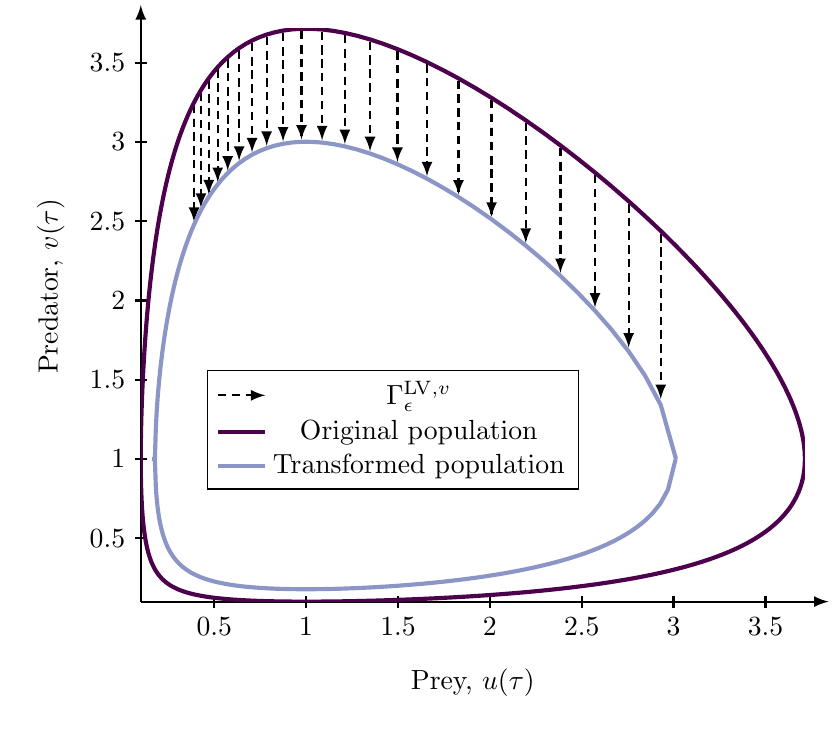
\begin{tikzpicture}
  % The axis of the plot
\begin{axis}[
    xlabel={Prey, $u(\tau)$},
    ylabel={Predator, $v(\tau)$},
    x label style={at={(axis description cs:0.5,-0.1)},anchor=north},
    y label style={at={(axis description cs:-0.1,0.55)},rotate=90,anchor=south},
    scaled x ticks = false,
    legend style={at={(axis description cs:0.1,0.3)},anchor=west,nodes={scale=1.00, transform shape}},    
    grid style=dashed,
]
\addplot[
color=black,->,>=latex,densely dashed
]
coordinates {%
(nan,2.439182400298198)
(2.9301016836553053,2.42219270562327)
(2.9301016836553053,2.4051187972915677)
(2.9301016836553053,2.3879581831050394)
(2.9301016836553053,2.370708248540889)
(2.9301016836553053,2.353366248229631)
(2.9301016836553053,2.3359292966560568)
(2.9301016836553053,2.3183943579948076)
(2.9301016836553053,2.300758234979849)
(2.9301016836553053,2.283017556694647)
(2.9301016836553053,2.2651687651496757)
(2.930101683655305,2.2472081005000626)
(2.9301016836553053,2.2291315847291213)
(2.9301016836553058,2.210935003599554)
(2.9301016836553053,2.1926138866421834)
(2.930101683655305,2.1741634849151614)
(2.9301016836553053,2.155578746222638)
(2.9301016836553053,2.136854287429228)
(2.9301016836553053,2.1179843634435156)
(2.9301016836553053,2.098962832367701)
(2.9301016836553053,2.0797831162182687)
(2.9301016836553053,2.060438156510247)
(2.930101683655305,2.0409203638601503)
(2.9301016836553053,2.0212215605934314)
(2.9301016836553053,2.0013329151326253)
(2.9301016836553053,1.9812448666809963)
(2.9301016836553058,1.9609470383895404)
(2.9301016836553053,1.9404281367787568)
(2.9301016836553053,1.919675834662587)
(2.9301016836553053,1.8986766341420103)
(2.930101683655305,1.8774157053610656)
(2.9301016836553053,1.855876695572414)
(2.9301016836553053,1.8340415015481666)
(2.9301016836553053,1.8118899963553472)
(2.9301016836553053,1.7893996987939251)
(2.9301016836553053,1.7665453700757097)
(2.9301016836553053,1.743298517168263)
(2.9301016836553053,1.7196267749780931)
(2.9301016836553053,1.6954931291804238)
(2.9301016836553053,1.6708549264069759)
(2.9301016836553053,1.6456625960743816)
(2.9301016836553053,1.6198579740554138)
(2.9301016836553053,1.5933720652893824)
(2.9301016836553053,1.5661219972789338)
(2.930101683655305,1.5380067753882856)
(2.9301016836553053,1.5089012083288453)
(2.9301016836553053,1.4786469365214259)
(2.9301016836553058,1.4470386717476187)
(2.9301016836553053,1.413802096934534)
(2.9301016836553053,1.3785562677085983)
};
\addlegendentry{$\Gamma^{\mathrm{LV},v}_{\epsilon}$}
\addplot[
forget plot,
color=black,->,>=latex,densely dashed
]
coordinates {%
(nan,2.626251840284192)
(2.7554824208200257,2.61007195710823)
(2.7554824208200257,2.593829535005732)
(2.7554824208200253,2.577523043502607)
(2.7554824208200257,2.56115089041575)
(2.7554824208200257,2.544711418337758)
(2.7554824208200253,2.528202900860623)
(2.7554824208200257,2.5116235385143333)
(2.7554824208200257,2.494971454393681)
(2.7554824208200257,2.4782446894435317)
(2.7554824208200257,2.461441197369107)
(2.7554824208200257,2.444558839135788)
(2.7554824208200253,2.427595377013899)
(2.7554824208200257,2.4105484681256613)
(2.7554824208200257,2.3934156574398333)
(2.7554824208200257,2.376194370156194)
(2.7554824208200257,2.358881903413556)
(2.7554824208200257,2.3414754172464685)
(2.7554824208200257,2.3239719247057735)
(2.7554824208200257,2.3063682810466615)
(2.7554824208200257,2.2886611718744274)
(2.7554824208200257,2.2708471001225745)
(2.7554824208200257,2.2529223717196647)
(2.7554824208200257,2.234883079780008)
(2.7554824208200253,2.216725087128186)
(2.7554824208200257,2.198444006937843)
(2.7554824208200257,2.180035181230148)
(2.755482420820026,2.1614936569356993)
(2.7554824208200257,2.142814159173981)
(2.7554824208200257,2.123991061344909)
(2.7554824208200257,2.1050183515552408)
(2.7554824208200257,2.0858895948164236)
(2.7554824208200257,2.066597890343564)
(2.7554824208200257,2.0471358231585595)
(2.7554824208200257,2.027495409040027)
(2.7554824208200257,2.0076680316680933)
(2.7554824208200257,1.9876443705682845)
(2.7554824208200257,1.967414318154011)
(2.7554824208200257,1.9469668837829484)
(2.7554824208200257,1.9262900822545241)
(2.7554824208200257,1.9053708035510495)
(2.7554824208200257,1.8841946598183728)
(2.7554824208200257,1.8627458045311711)
(2.7554824208200257,1.8410067174055196)
(2.7554824208200257,1.8189579467836197)
(2.7554824208200257,1.7965777987444524)
(2.7554824208200257,1.773841958830612)
(2.7554824208200257,1.750723027641677)
(2.7554824208200253,1.7271899450499115)
(2.7554824208200257,1.703207268557248)
};
\addplot[
forget plot,
color=black,->,>=latex,densely dashed
]
coordinates {%
(nan,2.807422586691301)
(2.5721834116423103,2.7918659106785535)
(2.5721834116423103,2.7762607055201767)
(2.5721834116423103,2.7606059592927616)
(2.5721834116423103,2.7449006254929693)
(2.5721834116423103,2.7291436213738343)
(2.5721834116423103,2.713333826177042)
(2.5721834116423103,2.697470079253128)
(2.5721834116423103,2.6815511780608134)
(2.5721834116423103,2.6655758760358323)
(2.5721834116423103,2.6495428803187404)
(2.5721834116423103,2.6334508493299635)
(2.5721834116423103,2.617298390180128)
(2.572183411642311,2.60108405590018)
(2.5721834116423103,2.5848063424776755)
(2.57218341164231,2.568463685681106)
(2.5721834116423103,2.552054457653946)
(2.5721834116423103,2.535576963257626)
(2.5721834116423103,2.519029436140468)
(2.5721834116423103,2.50241003450708)
(2.5721834116423103,2.485716836559884)
(2.5721834116423103,2.4689478355811936)
(2.5721834116423103,2.4521009346206473)
(2.5721834116423103,2.4351739407486095)
(2.5721834116423103,2.4181645588314673)
(2.5721834116423103,2.4010703847793335)
(2.572183411642311,2.383888898210519)
(2.5721834116423103,2.3666174544700644)
(2.5721834116423103,2.3492532759314964)
(2.5721834116423103,2.3317934425016205)
(2.57218341164231,2.314234881237336)
(2.5721834116423103,2.2965743549709283)
(2.5721834116423103,2.278808449825723)
(2.5721834116423103,2.260933561486989)
(2.5721834116423103,2.2429458800731146)
(2.5721834116423103,2.2248413734287587)
(2.5721834116423103,2.206615768634119)
(2.5721834116423103,2.188264531492575)
(2.5721834116423103,2.169782843718859)
(2.5721834116423103,2.1511655775064518)
(2.5721834116423103,2.1324072670957643)
(2.5721834116423103,2.1135020768999366)
(2.5721834116423103,2.0944437656651145)
(2.5721834116423103,2.075225646045501)
(2.5721834116423103,2.055840538855765)
(2.5721834116423103,2.0362807211190113)
(2.5721834116423103,2.0165378668506264)
(2.5721834116423103,1.9966029792975561)
(2.5721834116423103,1.9764663130771487)
(2.5721834116423103,1.9561172843134529)
};
\addplot[
forget plot,
color=black,->,>=latex,densely dashed
]
coordinates {%
(nan,2.978801496476531)
(2.38414354871953,2.9637285955267)
(2.38414354871953,2.948616555292683)
(2.38414354871953,2.933464662298722)
(2.38414354871953,2.9182721818467043)
(2.38414354871953,2.9030383571298177)
(2.38414354871953,2.8877624082981987)
(2.3841435487195306,2.8724435314733747)
(2.38414354871953,2.8570808977080167)
(2.38414354871953,2.8416736518872754)
(2.38414354871953,2.8262209115676247)
(2.38414354871953,2.810721765748835)
(2.38414354871953,2.795175273574308)
(2.38414354871953,2.7795804629544523)
(2.3841435487195306,2.763936329108292)
(2.38414354871953,2.748241833015442)
(2.38414354871953,2.7324958997739026)
(2.38414354871953,2.7166974168550055)
(2.38414354871953,2.7008452322481395)
(2.38414354871953,2.6849381524865374)
(2.38414354871953,2.668974940544683)
(2.38414354871953,2.6529543135970086)
(2.38414354871953,2.6368749406265364)
(2.38414354871953,2.620735439871023)
(2.38414354871953,2.604534376092924)
(2.38414354871953,2.5882702576581096)
(2.38414354871953,2.5719415334067173)
(2.38414354871953,2.5555465892978066)
(2.3841435487195306,2.5390837448075176)
(2.38414354871953,2.522551249058275)
(2.38414354871953,2.505947276654096)
(2.38414354871953,2.489269923194303)
(2.38414354871953,2.472517200434797)
(2.38414354871953,2.455687031062478)
(2.38414354871953,2.4387772430443895)
(2.38414354871953,2.421785563508543)
(2.38414354871953,2.404709612108155)
(2.38414354871953,2.38754689381503)
(2.38414354871953,2.3702947910809686)
(2.38414354871953,2.3529505552981935)
(2.38414354871953,2.335511297480694)
(2.38414354871953,2.3179739780779265)
(2.38414354871953,2.3003353958200283)
(2.38414354871953,2.2825921754802643)
(2.38414354871953,2.2647407544222027)
(2.38414354871953,2.246777367782633)
(2.38414354871953,2.228698032116153)
(2.38414354871953,2.210498527302285)
(2.38414354871953,2.1921743764841772)
(2.38414354871953,2.173720823770918)
};
\addplot[
forget plot,
color=black,->,>=latex,densely dashed
]
coordinates {%
(nan,3.136819528140607)
(2.1952864569614197,3.122123514643114)
(2.1952864569614197,3.1073948308412276)
(2.1952864569614197,3.092632944287184)
(2.1952864569614197,3.077837308423589)
(2.1952864569614197,3.0630073620596705)
(2.1952864569614197,3.0481425288222144)
(2.1952864569614197,3.0332422165798585)
(2.1952864569614197,3.0183058168391157)
(2.1952864569614197,3.003332704110415)
(2.1952864569614197,2.988322235242331)
(2.1952864569614197,2.9732737487220224)
(2.1952864569614197,2.9581865639397726)
(2.1952864569614197,2.943059980415351)
(2.1952864569614197,2.9278932769837573)
(2.1952864569614197,2.912685710937532)
(2.1952864569614197,2.8974365171237118)
(2.1952864569614197,2.882144906990348)
(2.1952864569614197,2.866810067581718)
(2.1952864569614197,2.8514311604769893)
(2.1952864569614197,2.83600732066911)
(2.1952864569614197,2.8205376553796326)
(2.1952864569614197,2.8050212428049712)
(2.1952864569614197,2.789457130789165)
(2.1952864569614197,2.7738443354178384)
(2.1952864569614197,2.758181839527565)
(2.1952864569614197,2.7424685911243354)
(2.1952864569614197,2.726703501704282)
(2.1952864569614197,2.7108854444691772)
(2.1952864569614197,2.6950132524285437)
(2.1952864569614197,2.6790857163794684)
(2.1952864569614197,2.6631015827543485)
(2.1952864569614197,2.6470595513258854)
(2.1952864569614197,2.6309582727575918)
(2.1952864569614197,2.614796345986936)
(2.1952864569614197,2.598572315426936)
(2.1952864569614197,2.582284667970601)
(2.1952864569614197,2.5659318297809928)
(2.1952864569614197,2.5495121628478685)
(2.1952864569614197,2.533023961289868)
(2.1952864569614197,2.5164654473788723)
(2.1952864569614197,2.499834767260664)
(2.1952864569614197,2.483129986343033)
(2.1952864569614197,2.466349084319269)
(2.1952864569614197,2.449489949791185)
(2.1952864569614197,2.4325503744516332)
(2.1952864569614197,2.4155280467816334)
(2.1952864569614197,2.3984205452117306)
(2.1952864569614197,2.3812253306908144)
(2.1952864569614197,2.3639397385990852)
};
\addplot[
forget plot,
color=black,->,>=latex,densely dashed
]
coordinates {%
(nan,3.27845971883254)
(2.0092690289430606,3.2640568628001896)
(2.0092690289430606,3.249625880748858)
(2.0092690289430606,3.2351663546711453)
(2.0092690289430606,3.220677856487359)
(2.0092690289430606,3.2061599477061176)
(2.0092690289430606,3.1916121790700727)
(2.0092690289430606,3.177034090186069)
(2.0092690289430606,3.1624252091388656)
(2.0092690289430606,3.1477850520875412)
(2.0092690289430606,3.133113122843594)
(2.0092690289430606,3.1184089124297527)
(2.0092690289430606,3.103671898618379)
(2.0092690289430606,3.088901545448315)
(2.0092690289430606,3.0740973027189304)
(2.0092690289430606,3.059258605460045)
(2.0092690289430606,3.0443848733763)
(2.0092690289430606,3.029475510264279)
(2.0092690289430606,3.01452990340178)
(2.0092690289430606,2.9995474229051555)
(2.0092690289430606,2.9845274210557062)
(2.0092690289430606,2.9694692315911504)
(2.0092690289430606,2.9543721689607496)
(2.0092690289430606,2.9392355275416535)
(2.0092690289430606,2.9240585808139783)
(2.0092690289430606,2.9088405804919346)
(2.0092690289430606,2.89358075560811)
(2.0092690289430606,2.8782783115477923)
(2.0092690289430606,2.8629324290299603)
(2.0092690289430606,2.8475422630313116)
(2.0092690289430606,2.8321069416493856)
(2.0092690289430606,2.8166255649005225)
(2.0092690289430606,2.8010972034480486)
(2.0092690289430606,2.7855208972556675)
(2.0092690289430606,2.769895654160634)
(2.0092690289430606,2.754220448360789)
(2.0092690289430606,2.738494218809026)
(2.0092690289430606,2.7227158675081866)
(2.0092690289430606,2.7068842576987358)
(2.0092690289430606,2.6909982119308786)
(2.0092690289430606,2.6750565100119927)
(2.0092690289430606,2.6590578868193866)
(2.0092690289430606,2.643001029967458)
(2.0092690289430606,2.626884577317209)
(2.0092690289430606,2.610707114314967)
(2.0092690289430606,2.594467171145739)
(2.0092690289430606,2.578163219685243)
(2.0092690289430606,2.5617936702329125)
(2.0092690289430606,2.5453568680063947)
(2.0092690289430606,2.528851089375898)
};
\addplot[
forget plot,
color=black,->,>=latex,densely dashed
]
coordinates {%
(nan,3.40142167043343)
(1.8292762657323478,3.3872451340337952)
(1.8292762657323478,3.373043699524238)
(1.8292762657323476,3.358817023480672)
(1.8292762657323478,3.344564754816589)
(1.8292762657323478,3.3302865345442965)
(1.8292762657323476,3.3159819955264838)
(1.8292762657323478,3.301650762217721)
(1.8292762657323478,3.2872924503953485)
(1.8292762657323476,3.272906666879257)
(1.8292762657323478,3.258493009239957)
(1.8292762657323478,3.244051065494373)
(1.8292762657323476,3.2295804137886863)
(1.8292762657323478,3.215080622067589)
(1.8292762657323478,3.200551247729192)
(1.8292762657323478,3.1859918372648584)
(1.8292762657323478,3.171401925883118)
(1.8292762657323478,3.1567810371168252)
(1.8292762657323476,3.142128682412466)
(1.829276265732348,3.127444360701439)
(1.8292762657323478,3.1127275579504783)
(1.8292762657323478,3.0979777466922656)
(1.8292762657323478,3.0831943855335475)
(1.8292762657323478,3.0683769186400363)
(1.8292762657323476,3.053524775196647)
(1.8292762657323478,3.0386373688416186)
(1.8292762657323478,3.0237140970729555)
(1.8292762657323478,3.0087543406255235)
(1.8292762657323478,2.9937574628170056)
(1.8292762657323478,2.978722808860807)
(1.8292762657323478,2.9636497051438324)
(1.8292762657323478,2.948537458466936)
(1.8292762657323478,2.9333853552456537)
(1.8292762657323478,2.9181926606686526)
(1.8292762657323478,2.9029586178111435)
(1.8292762657323476,2.887682446700271)
(1.8292762657323476,2.8723633433292766)
(1.8292762657323476,2.8570004786169583)
(1.829276265732348,2.8415929973086906)
(1.829276265732348,2.8261400168149273)
(1.8292762657323478,2.810640625982813)
(1.8292762657323478,2.795093883796128)
(1.8292762657323478,2.7794988179984075)
(1.8292762657323478,2.7638544236336053)
(1.8292762657323478,2.7481596614982142)
(1.8292762657323478,2.7324134564981826)
(1.8292762657323478,2.7166146959033886)
(1.8292762657323476,2.7007622274917646)
(1.8292762657323476,2.6848548575744373)
(1.829276265732348,2.6688913488924415)
};
\addplot[
forget plot,
color=black,->,>=latex,densely dashed
]
coordinates {%
(nan,3.5042060530796926)
(1.6578841746791864,3.4902015666717383)
(1.6578841746791864,3.4761744777572012)
(1.6578841746791866,3.4621244924222445)
(1.6578841746791864,3.448051310581789)
(1.6578841746791864,3.4339546257987337)
(1.6578841746791866,3.4198341250962976)
(1.6578841746791864,3.4056894887632243)
(1.6578841746791864,3.391520390151484)
(1.6578841746791864,3.3773264954661415)
(1.6578841746791864,3.3631074635469993)
(1.6578841746791861,3.3488629456416326)
(1.6578841746791866,3.3345925851693825)
(1.6578841746791864,3.3202960174758918)
(1.6578841746791864,3.305972869577677)
(1.6578841746791864,3.2916227598962866)
(1.6578841746791864,3.277245297981473)
(1.6578841746791864,3.262840084222865)
(1.6578841746791864,3.248406709549519)
(1.6578841746791864,3.23394475511674)
(1.6578841746791864,3.2194537919793085)
(1.6578841746791864,3.2049333807514637)
(1.6578841746791861,3.190383071250464)
(1.6578841746791864,3.1758024021259335)
(1.6578841746791866,3.161190900472032)
(1.6578841746791864,3.1465480814223534)
(1.6578841746791864,3.1318734477264387)
(1.6578841746791864,3.1171664893069075)
(1.6578841746791864,3.1024266827960854)
(1.6578841746791864,3.0876534910509807)
(1.6578841746791864,3.072846362645342)
(1.6578841746791864,3.058004731337483)
(1.6578841746791864,3.0431280155124303)
(1.6578841746791864,3.028215617596879)
(1.6578841746791864,3.013266923445316)
(1.6578841746791864,2.998281301695557)
(1.6578841746791864,2.983258103091822)
(1.6578841746791864,2.968196659773327)
(1.6578841746791864,2.953096284526228)
(1.6578841746791864,2.93795626999658)
(1.6578841746791864,2.9227758878618193)
(1.6578841746791866,2.907554387958044)
(1.6578841746791864,2.8922909973602122)
(1.6578841746791864,2.8769849194120916)
(1.6578841746791861,2.8616353327025927)
(1.6578841746791864,2.84624138998481)
(1.6578841746791864,2.830802217033814)
(1.6578841746791864,2.8153169114389103)
(1.6578841746791866,2.799784541325706)
(1.6578841746791864,2.784204144002953)
};
\addplot[
forget plot,
color=black,->,>=latex,densely dashed
]
coordinates {%
(nan,3.586118296327405)
(1.4969977505087715,3.5722410878432314)
(1.4969977505087715,3.558342889258299)
(1.4969977505087713,3.5444234396206724)
(1.4969977505087715,3.5304824727471877)
(1.4969977505087715,3.516519717077262)
(1.4969977505087713,3.5025348955213937)
(1.4969977505087715,3.488527725304169)
(1.4969977505087715,3.4744979178015094)
(1.4969977505087715,3.4604451783719186)
(1.4969977505087715,3.4463692061814357)
(1.4969977505087717,3.4322696940220334)
(1.4969977505087713,3.418146328123122)
(1.4969977505087715,3.403998787955884)
(1.4969977505087715,3.389826746030052)
(1.4969977505087715,3.3756298676828194)
(1.4969977505087715,3.3614078108594754)
(1.4969977505087715,3.3471602258853834)
(1.4969977505087715,3.332886755228868)
(1.4969977505087715,3.3185870332545884)
(1.4969977505087715,3.304260685966889)
(1.4969977505087715,3.2899073307424973)
(1.4969977505087717,3.2755265760529833)
(1.4969977505087715,3.26111802117417)
(1.4969977505087713,3.2466812558847042)
(1.4969977505087715,3.232215860151204)
(1.4969977505087715,3.2177214038000237)
(1.4969977505087715,3.2031974461748383)
(1.4969977505087715,3.1886435357792724)
(1.4969977505087715,3.1740592099037803)
(1.4969977505087715,3.159443994235907)
(1.4969977505087715,3.144797402453049)
(1.4969977505087715,3.130118935796708)
(1.4969977505087715,3.1154080826272272)
(1.4969977505087715,3.100664317957902)
(1.4969977505087715,3.085887102967282)
(1.4969977505087715,3.0710758844884127)
(1.4969977505087715,3.056230094473665)
(1.4969977505087715,3.041349149433724)
(1.4969977505087715,3.026432449849183)
(1.4969977505087715,3.0114793795531156)
(1.4969977505087715,2.996489305082834)
(1.4969977505087715,2.9814615749989564)
(1.4969977505087713,2.9663955191697395)
(1.4969977505087717,2.951290448018492)
(1.4969977505087715,2.9361456517317195)
(1.4969977505087715,2.9209603994254696)
(1.4969977505087715,2.9057339382671508)
(1.4969977505087713,2.8904654925498994)
(1.4969977505087715,2.8751542627163094)
};
\addplot[
forget plot,
color=black,->,>=latex,densely dashed
]
coordinates {%
(nan,3.647203480569721)
(1.3478579312616616,3.6334160399322886)
(1.3478579312616616,3.619608703333742)
(1.3478579312616616,3.6057812313151674)
(1.3478579312616616,3.5919333797749706)
(1.3478579312616616,3.5780648998434676)
(1.3478579312616616,3.564175537753069)
(1.3478579312616616,3.5502650347039157)
(1.3478579312616616,3.536333126724767)
(1.3478579312616616,3.5223795445289228)
(1.3478579312616616,3.5084040133649688)
(1.3478579312616616,3.494406252862121)
(1.3478579312616616,3.480385976869919)
(1.3478579312616614,3.4663428932920235)
(1.3478579312616616,3.4522767039138436)
(1.3478579312616616,3.438187104223719)
(1.3478579312616616,3.424073783227357)
(1.3478579312616616,3.4099364232552114)
(1.3478579312616616,3.3957746997624754)
(1.3478579312616616,3.3815882811213367)
(1.3478579312616616,3.3673768284051286)
(1.3478579312616616,3.3531399951639953)
(1.3478579312616616,3.338877427191446)
(1.3478579312616616,3.3245887622824584)
(1.3478579312616616,3.3102736299801756)
(1.3478579312616616,3.295931651313796)
(1.3478579312616614,3.281562438524974)
(1.3478579312616616,3.267165594783003)
(1.3478579312616616,3.2527407138880657)
(1.3478579312616616,3.2382873799619425)
(1.3478579312616616,3.2238051671255294)
(1.3478579312616616,3.2092936391624542)
(1.3478579312616616,3.1947523491680774)
(1.3478579312616616,3.1801808391830755)
(1.3478579312616616,3.165578639810791)
(1.3478579312616616,3.1509452698174365)
(1.3478579312616616,3.1362802357142434)
(1.3478579312616616,3.1215830313205086)
(1.3478579312616616,3.1068531373065036)
(1.3478579312616616,3.092090020715067)
(1.3478579312616616,3.0772931344606818)
(1.3478579312616616,3.0624619168047134)
(1.3478579312616616,3.0475957908054214)
(1.3478579312616616,3.032694163741236)
(1.3478579312616616,3.0177564265057177)
(1.3478579312616616,3.002781952972459)
(1.3478579312616616,2.9877700993281087)
(1.3478579312616616,2.972720203371532)
(1.3478579312616616,2.9576315837769847)
(1.3478579312616619,2.94250353931903)
};
\addplot[
forget plot,
color=black,->,>=latex,densely dashed
]
coordinates {%
(nan,3.688133305131117)
(1.211101634341837,3.674403721217572)
(1.211101634341837,3.660654927901811)
(1.211101634341837,3.6468866988439395)
(1.211101634341837,3.6330988034106553)
(1.211101634341837,3.6192910065618213)
(1.211101634341837,3.6054630687331413)
(1.211101634341837,3.5916147457148253)
(1.211101634341837,3.5777457885260473)
(1.211101634341837,3.563855943285043)
(1.211101634341837,3.549944951074634)
(1.211101634341837,3.536012547803004)
(1.211101634341837,3.5220584640595005)
(1.211101634341837,3.5080824249652687)
(1.211101634341837,3.494084150018459)
(1.211101634341837,3.480063352933793)
(1.211101634341837,3.466019741476218)
(1.211101634341837,3.4519530172883974)
(1.211101634341837,3.4378628757117293)
(1.211101634341837,3.423749005600637)
(1.211101634341837,3.409611089129772)
(1.211101634341837,3.3954488015938393)
(1.211101634341837,3.3812618111995163)
(1.211101634341837,3.36704977884995)
(1.211101634341837,3.352812357919493)
(1.211101634341837,3.338549194020692)
(1.211101634341837,3.324259924761377)
(1.211101634341837,3.309944179492053)
(1.211101634341837,3.2956015790429865)
(1.211101634341837,3.2812317354504845)
(1.211101634341837,3.266834251671803)
(1.211101634341837,3.252408721288118)
(1.211101634341837,3.237954728194945)
(1.211101634341837,3.2234718462793333)
(1.211101634341837,3.2089596390831656)
(1.211101634341837,3.194417659451806)
(1.211101634341837,3.179845449167326)
(1.211101634341837,3.1652425385654612)
(1.211101634341837,3.150608446135421)
(1.211101634341837,3.135942678101604)
(1.211101634341837,3.1212447279861975)
(1.211101634341837,3.1065140761516017)
(1.211101634341837,3.0917501893215324)
(1.211101634341837,3.076952520079551)
(1.211101634341837,3.062120506343748)
(1.211101634341837,3.0472535708161517)
(1.211101634341837,3.032351120405378)
(1.211101634341837,3.0174125456209104)
(1.211101634341837,3.002437219937299)
(1.211101634341837,2.9874244991264223)
};
\addplot[
forget plot,
color=black,->,>=latex,densely dashed
]
coordinates {%
(nan,3.7100672669470613)
(1.086855748273381,3.6963679659504076)
(1.086855748273381,3.6826498091335877)
(1.086855748273381,3.668912576801152)
(1.086855748273381,3.6551560451381557)
(1.086855748273381,3.6413799861025975)
(1.086855748273381,3.627584167314205)
(1.086855748273381,3.613768351939466)
(1.086855748273381,3.599932298572717)
(1.086855748273381,3.586075761113156)
(1.086855748273381,3.572198488637574)
(1.086855748273381,3.5583002252686535)
(1.086855748273381,3.5443807100386118)
(1.086855748273381,3.530439676748025)
(1.086855748273381,3.516476853819582)
(1.0868557482733812,3.5024919641465875)
(1.086855748273381,3.488484724935937)
(1.086855748273381,3.474454847545357)
(1.086855748273381,3.460402037314627)
(1.086855748273381,3.4463259933905195)
(1.086855748273381,3.432226408545169)
(1.086855748273381,3.418102968987564)
(1.086855748273381,3.4039553541677146)
(1.086855748273381,3.389783236573889)
(1.086855748273381,3.375586281520855)
(1.086855748273381,3.3613641469308844)
(1.086855748273381,3.347116483105602)
(1.086855748273381,3.332842932488856)
(1.086855748273381,3.3185431294200547)
(1.086855748273381,3.3042166998774904)
(1.0868557482733812,3.2898632612111776)
(1.086855748273381,3.2754824218646528)
(1.086855748273381,3.26107378108519)
(1.086855748273381,3.2466369286218297)
(1.086855748273381,3.2321714444105925)
(1.086855748273381,3.2176768982462103)
(1.086855748273381,3.20315284943966)
(1.086855748273381,3.188598846460752)
(1.086855748273381,3.1740144265649515)
(1.086855748273381,3.159399115403597)
(1.086855748273381,3.1447524266166007)
(1.086855748273381,3.1300738614066406)
(1.086855748273381,3.115362908093845)
(1.086855748273381,3.100619041649829)
(1.086855748273381,3.0858417232099313)
(1.086855748273381,3.0710303995623836)
(1.086855748273381,3.0561845026130627)
(1.086855748273381,3.0413034488243955)
(1.086855748273381,3.026386638626872)
(1.086855748273381,3.0114334558015186)
};
\addplot[
forget plot,
color=black,->,>=latex,densely dashed
]
coordinates {%
(nan,3.7145088027022672)
(0.9748460571069857,3.7008155740537765)
(0.9748460571069857,3.6871035600104856)
(0.9748460571069857,3.673372542191217)
(0.9748460571069857,3.6596222981294533)
(0.9748460571069856,3.645852601166928)
(0.9748460571069857,3.6320632203435914)
(0.9748460571069858,3.6182539202838893)
(0.9748460571069857,3.6044244610791436)
(0.9748460571069857,3.5905745981659067)
(0.9748460571069856,3.576704082200103)
(0.9748460571069857,3.5628126589267843)
(0.9748460571069857,3.548900069045308)
(0.9748460571069857,3.5349660480697462)
(0.9748460571069858,3.5210103261843084)
(0.9748460571069857,3.5070326280935737)
(0.9748460571069857,3.493032672867287)
(0.9748460571069858,3.4790101737794887)
(0.9748460571069857,3.464964838141713)
(0.9748460571069857,3.4508963671300084)
(0.9748460571069856,3.436804455605457)
(0.9748460571069857,3.4226887919279476)
(0.9748460571069857,3.408549057762835)
(0.9748460571069856,3.39438492788)
(0.9748460571069857,3.3801960699460163)
(0.9748460571069857,3.3659821443065523)
(0.9748460571069857,3.351742803761748)
(0.9748460571069857,3.3374776933319414)
(0.9748460571069858,3.3231864500141413)
(0.9748460571069857,3.308868702528665)
(0.9748460571069857,3.294524071055431)
(0.9748460571069857,3.2801521669594)
(0.9748460571069857,3.265752592504615)
(0.9748460571069857,3.2513249405562483)
(0.9748460571069858,3.2368687942700514)
(0.9748460571069856,3.2223837267685322)
(0.9748460571069857,3.20786930080318)
(0.9748460571069857,3.1933250684019847)
(0.9748460571069857,3.1787505705014714)
(0.9748460571069858,3.164145336562403)
(0.9748460571069856,3.149508884168264)
(0.9748460571069857,3.1348407186055733)
(0.9748460571069857,3.1201403324250165)
(0.9748460571069857,3.1054072049823054)
(0.9748460571069857,3.090640801957627)
(0.9748460571069858,3.0758405748524384)
(0.9748460571069856,3.0610059604622952)
(0.9748460571069857,3.0461363803243118)
(0.9748460571069857,3.0312312401377333)
(0.9748460571069857,3.016289929156024)
};
\addplot[
forget plot,
color=black,->,>=latex,densely dashed
]
coordinates {%
(nan,3.70317165105318)
(0.8745059539098055,3.6894628828617786)
(0.8745059539098055,3.6757351487360927)
(0.8745059539098055,3.6619882269196347)
(0.8745059539098055,3.648221891482691)
(0.8745059539098055,3.6344359122129615)
(0.8745059539098055,3.6206300545024623)
(0.8745059539098055,3.606804079230598)
(0.8745059539098055,3.5929577426432155)
(0.8745059539098055,3.5790907962274865)
(0.8745059539098055,3.565202986582423)
(0.8745059539098055,3.551294055284867)
(0.8745059539098055,3.537363738750724)
(0.8745059539098055,3.5234117680912687)
(0.8745059539098055,3.5094378689642727)
(0.8745059539098055,3.495441761419766)
(0.8745059539098055,3.4814231597401464)
(0.8745059539098055,3.46738177227443)
(0.8745059539098055,3.453317301266339)
(0.8745059539098056,3.4392294426759746)
(0.8745059539098055,3.4251178859947577)
(0.8745059539098053,3.410982314053346)
(0.8745059539098055,3.3968224028220417)
(0.8745059539098056,3.3826378212041233)
(0.8745059539098055,3.368428230819947)
(0.8745059539098053,3.354193285783652)
(0.8745059539098055,3.3399326324704934)
(0.8745059539098056,3.325645909274968)
(0.8745059539098055,3.3113327463591675)
(0.8745059539098053,3.2969927653908915)
(0.8745059539098055,3.282625579270994)
(0.8745059539098056,3.268230791849422)
(0.8745059539098055,3.2538079976293703)
(0.8745059539098055,3.239356781458938)
(0.8745059539098055,3.2248767182096456)
(0.8745059539098055,3.2103673724411)
(0.8745059539098055,3.19582829805111)
(0.8745059539098055,3.1812590379104293)
(0.8745059539098056,3.166659123481338)
(0.8745059539098055,3.1520280744191473)
(0.8745059539098055,3.1373653981557172)
(0.8745059539098055,3.1226705894639495)
(0.8745059539098053,3.1079431300022233)
(0.8745059539098055,3.0931824878376064)
(0.8745059539098055,3.078388116946639)
(0.8745059539098055,3.0635594566923805)
(0.8745059539098056,3.0486959312763364)
(0.8745059539098055,3.033796949163767)
(0.8745059539098055,3.018861902480792)
(0.8745059539098055,3.003890166381582)
};
\addplot[
forget plot,
color=black,->,>=latex,densely dashed
]
coordinates {%
(nan,3.6778656651463724)
(0.7850748605408029,3.6641217341684196)
(0.7850748605408029,3.6503584248910186)
(0.7850748605408029,3.6365755077734545)
(0.7850748605408029,3.622772748897101)
(0.7850748605408029,3.608949909849124)
(0.7850748605408029,3.5951067476021548)
(0.7850748605408029,3.5812430143898406)
(0.7850748605408029,3.567358457578046)
(0.7850748605408029,3.553452819531556)
(0.7850748605408029,3.5395258374760603)
(0.7850748605408029,3.5255772433552375)
(0.7850748605408029,3.511606763682705)
(0.7850748605408029,3.497614119388623)
(0.7850748605408029,3.4835990256606966)
(0.7850748605408029,3.469561191779355)
(0.7850748605408029,3.4555003209468134)
(0.7850748605408029,3.4414161101097553)
(0.7850748605408029,3.4273082497753427)
(0.7850748605408029,3.4131764238202424)
(0.7850748605408029,3.3990203092923337)
(0.7850748605408029,3.3848395762047767)
(0.7850748605408029,3.370633887321886)
(0.7850748605408029,3.356402897937341)
(0.7850748605408029,3.342146255642252)
(0.7850748605408029,3.3278636000852235)
(0.7850748605408029,3.3135545627221434)
(0.7850748605408029,3.299218766555921)
(0.7850748605408029,3.28485582586554)
(0.7850748605408029,3.2704653459238817)
(0.7850748605408029,3.2560469227037667)
(0.7850748605408029,3.2416001425715906)
(0.7850748605408029,3.227124581967924)
(0.7850748605408029,3.212619807074373)
(0.7850748605408029,3.1980853734659975)
(0.7850748605408029,3.1835208257484977)
(0.7850748605408029,3.1689256971793545)
(0.7850748605408029,3.1542995092720463)
(0.7850748605408029,3.1396417713824167)
(0.7850748605408029,3.124951980276189)
(0.7850748605408029,3.110229619676587)
(0.7850748605408029,3.095474159790912)
(0.7850748605408029,3.080685056814893)
(0.7850748605408029,3.065861752413502)
(0.7850748605408029,3.0510036731768704)
(0.7850748605408029,3.03611023004983)
(0.7850748605408029,3.021180817733502)
(0.7850748605408029,3.0062148140572424)
(0.7850748605408029,2.991211579319136)
(0.7850748605408029,2.976170455593093)
};
\addplot[
forget plot,
color=black,->,>=latex,densely dashed
]
coordinates {%
(nan,3.6404063098907984)
(0.7056807030954716,3.626609086672156)
(0.7056807030954716,3.61279184996939)
(0.7056807030954716,3.5989543580493435)
(0.7056807030954716,3.5850963644748552)
(0.7056807030954716,3.5712176179772106)
(0.7056807030954716,3.557317862324105)
(0.7056807030954716,3.5433968361829664)
(0.7056807030954716,3.5294542729794163)
(0.7056807030954716,3.515489900750671)
(0.7056807030954716,3.5015034419936457)
(0.7056807030954716,3.4874946135075553)
(0.7056807030954716,3.4734631262307154)
(0.7056807030954716,3.459408685071349)
(0.7056807030954716,3.445330988732057)
(0.7056807030954716,3.4312297295277197)
(0.7056807030954716,3.41710459319649)
(0.7056807030954716,3.402955258703574)
(0.7056807030954716,3.38878139803745)
(0.7056807030954716,3.3745826759981776)
(0.7056807030954716,3.3603587499774097)
(0.7056807030954716,3.346109269729583)
(0.7056807030954716,3.331833877134585)
(0.7056807030954716,3.3175322059497754)
(0.7056807030954716,3.3032038815529723)
(0.7056807030954715,3.288848520674433)
(0.7056807030954716,3.274465731117861)
(0.7056807030954716,3.2600551114697747)
(0.7056807030954716,3.245616250796656)
(0.7056807030954716,3.2311487283292344)
(0.7056807030954716,3.216652113133238)
(0.7056807030954716,3.2021259637658996)
(0.7056807030954716,3.1875698279174522)
(0.7056807030954716,3.172983242036814)
(0.7056807030954716,3.1583657309405995)
(0.7056807030954716,3.1437168074045356)
(0.7056807030954716,3.1290359717363265)
(0.7056807030954716,3.114322711328901)
(0.7056807030954716,3.099576500192963)
(0.7056807030954716,3.084796798467629)
(0.7056807030954716,3.069983051907931)
(0.7056807030954716,3.055134691347777)
(0.7056807030954716,3.0402511321369876)
(0.7056807030954716,3.0253317735508025)
(0.7056807030954716,3.0103759981702436)
(0.7056807030954716,2.9953831712315333)
(0.7056807030954716,2.9803526399426725)
(0.7056807030954716,2.9652837327651267)
(0.7056807030954716,2.9501757586584323)
(0.7056807030954716,2.935028006285346)
};
\addplot[
forget plot,
color=black,->,>=latex,densely dashed
]
coordinates {%
(nan,3.5925479441389774)
(0.6354047241687562,3.578680384383102)
(0.6354047241687562,3.5647919538281188)
(0.6354047241687562,3.5508823939002703)
(0.6354047241687562,3.5369514408606673)
(0.6354047241687562,3.522998825661465)
(0.6354047241687562,3.509024273796837)
(0.6354047241687562,3.4950275051485633)
(0.6354047241687562,3.48100823382598)
(0.6354047241687562,3.4669661680000448)
(0.6354047241687562,3.4529010097312396)
(0.6354047241687562,3.43881245479105)
(0.6354047241687562,3.424700192476706)
(0.6354047241687562,3.4105639054188797)
(0.6354047241687562,3.3964032693820108)
(0.6354047241687562,3.3822179530569207)
(0.6354047241687562,3.368007617845321)
(0.6354047241687562,3.3537719176358705)
(0.6354047241687562,3.3395104985713218)
(0.6354047241687562,3.3252229988063733)
(0.6354047241687562,3.310909048255725)
(0.6354047241687562,3.2965682683317046)
(0.6354047241687562,3.282200271671897)
(0.6354047241687562,3.2678046618540257)
(0.6354047241687562,3.253381033100234)
(0.6354047241687562,3.238928969968262)
(0.6354047241687562,3.224448047029548)
(0.6354047241687562,3.209937828533487)
(0.6354047241687562,3.195397868057096)
(0.6354047241687562,3.180827708139296)
(0.6354047241687562,3.1662268798989937)
(0.6354047241687562,3.1515949026360803)
(0.6354047241687562,3.1369312834143877)
(0.6354047241687562,3.1222355166256137)
(0.6354047241687562,3.1075070835331426)
(0.6354047241687562,3.092745451794612)
(0.6354047241687562,3.0779500749620126)
(0.6354047241687562,3.063120391958014)
(0.6354047241687562,3.0482558265271273)
(0.6354047241687562,3.0333557866601977)
(0.6354047241687562,3.0184196639906573)
(0.6354047241687562,3.003446833160798)
(0.6354047241687562,2.98843665115625)
(0.6354047241687562,2.973388456606683)
(0.6354047241687562,2.9583015690506342)
(0.6354047241687562,2.9431752881621627)
(0.6354047241687562,2.928008892936912)
(0.6354047241687562,2.9128016408349353)
(0.6354047241687562,2.8975527668774483)
(0.6354047241687562,2.8822614826944584)
};
\addplot[
forget plot,
color=black,->,>=latex,densely dashed
]
coordinates {%
(nan,3.5359385315612744)
(0.5733293202438954,3.521984332000823)
(0.5733293202438954,3.5080081756156023)
(0.5733293202438954,3.494009781873509)
(0.5733293202438954,3.4799888644581167)
(0.5733293202438954,3.465945131102339)
(0.5733293202438954,3.45187828341586)
(0.5733293202438954,3.4377880167061443)
(0.5733293202438954,3.4236740197926645)
(0.5733293202438954,3.409535974814087)
(0.5733293202438954,3.395373557028043)
(0.5733293202438954,3.3811864346031637)
(0.5733293202438954,3.3669742684029935)
(0.5733293202438954,3.3527367117614117)
(0.5733293202438954,3.33847341024912)
(0.5733293202438954,3.3241840014307926)
(0.5733293202438954,3.309868114612411)
(0.5733293202438954,3.2955253705782956)
(0.5733293202438954,3.2811553813173213)
(0.5733293202438954,3.2667577497377738)
(0.5733293202438954,3.2523320693700892)
(0.5733293202438954,3.23787792405776)
(0.5733293202438954,3.2233948876337175)
(0.5733293202438954,3.2088825235840064)
(0.5733293202438954,3.1943403846962424)
(0.5733293202438954,3.179768012692763)
(0.5733293202438954,3.1651649378474906)
(0.5733293202438954,3.1505306785856466)
(0.5733293202438954,3.1358647410653755)
(0.5733293202438954,3.1211666187402325)
(0.5733293202438954,3.1064357919015038)
(0.5733293202438954,3.0916717271991856)
(0.5733293202438954,3.0768738771404003)
(0.5733293202438954,3.062041679563941)
(0.5733293202438954,3.047174557089547)
(0.5733293202438954,3.0322719165404064)
(0.5733293202438954,3.017333148337282)
(0.5733293202438954,3.0023576258625404)
(0.5733293202438954,2.9873447047922483)
(0.5733293202438954,2.9722937223943373)
(0.5733293202438954,2.957203996790735)
(0.5733293202438954,2.9420748261811593)
(0.5733293202438954,2.92690548802613)
(0.5733293202438954,2.911695238186542)
(0.5733293202438954,2.8964433100169584)
(0.5733293202438954,2.8811489134095427)
(0.5733293202438954,2.8658112337853123)
(0.5733293202438954,2.8504294310291276)
(0.5733293202438954,2.8350026383645446)
(0.5733293202438954,2.8195299611643216)
};
\addplot[
forget plot,
color=black,->,>=latex,densely dashed
]
coordinates {%
(nan,3.472092194298804)
(0.5185711135951477,3.458035496418073)
(0.5185711135951477,3.4439555136065394)
(0.5185711135951477,3.4298519375455405)
(0.5185711135951477,3.415724453320831)
(0.5185711135951477,3.401572739225672)
(0.5185711135951477,3.3873964665562832)
(0.5185711135951477,3.3731952993993657)
(0.5185711135951477,3.358968894411276)
(0.5185711135951477,3.3447169005884847)
(0.5185711135951477,3.3304389590288612)
(0.5185711135951477,3.316134702683365)
(0.5185711135951477,3.3018037560976405)
(0.5185711135951477,3.2874457351430384)
(0.5185711135951477,3.2730602467365024)
(0.5185711135951477,3.2586468885487823)
(0.5185711135951477,3.244205248700344)
(0.5185711135951477,3.229734905444374)
(0.5185711135951477,3.215235426836164)
(0.5185711135951477,3.200706370388043)
(0.5185711135951477,3.1861472827098742)
(0.5185711135951477,3.1715576991324737)
(0.5185711135951477,3.1569371433153495)
(0.5185711135951477,3.1422851268362657)
(0.5185711135951477,3.127601148762228)
(0.5185711135951477,3.1128846952007705)
(0.5185711135951477,3.0981352388304133)
(0.5185711135951477,3.0833522384091063)
(0.5185711135951477,3.0685351382593877)
(0.5185711135951477,3.053683367728891)
(0.5185711135951477,3.03879634062475)
(0.5185711135951477,3.0238734546203476)
(0.5185711135951477,3.0089140906327336)
(0.5185711135951477,2.993917612168921)
(0.5185711135951477,2.9788833646391537)
(0.5185711135951477,2.9638106746350723)
(0.5185711135951477,2.9486988491705737)
(0.5185711135951477,2.933547174882977)
(0.5185711135951477,2.918354917191944)
(0.5185711135951477,2.903121319413381)
(0.5185711135951477,2.8878456018253633)
(0.5185711135951477,2.8725269606828565)
(0.5185711135951477,2.8571645671777874)
(0.5185711135951477,2.8417575663406978)
(0.5185711135951477,2.8263050758799437)
(0.5185711135951477,2.810806184954043)
(0.5185711135951477,2.795259952872412)
(0.5185711135951477,2.779665407719328)
(0.5185711135951477,2.7640215448955123)
(0.5185711135951477,2.7483273255712213)
};
\addplot[
forget plot,
color=black,->,>=latex,densely dashed
]
coordinates {%
(nan,3.4023756965898624)
(0.47030197368957394,3.3882008251341627)
(0.47030197368957394,3.3740010784314296)
(0.47030197368957394,3.3597761135653506)
(0.47030197368957394,3.34552557997294)
(0.47030197368957394,3.331249119206416)
(0.47030197368957394,3.3169463646854185)
(0.47030197368957394,3.302616941439208)
(0.47030197368957394,3.2882604658382864)
(0.470301973689574,3.273876545314943)
(0.47030197368957394,3.2594647780721293)
(0.4703019736895739,3.2450247527801)
(0.47030197368957394,3.23055604826015)
(0.470301973689574,3.2160582331548055)
(0.47030197368957394,3.2015308655837234)
(0.4703019736895739,3.186973492784559)
(0.47030197368957394,3.1723856507379886)
(0.47030197368957394,3.157766863776015)
(0.470301973689574,3.143116644172507)
(0.47030197368957394,3.1284344917157596)
(0.47030197368957394,3.1137198932602868)
(0.47030197368957394,3.098972322258871)
(0.4703019736895739,3.0841912382722043)
(0.47030197368957394,3.0693760864553976)
(0.47030197368957394,3.0545262970199287)
(0.47030197368957394,3.0396412846695657)
(0.470301973689574,3.024720448008727)
(0.47030197368957394,3.009763168921606)
(0.47030197368957394,2.9947688119202884)
(0.47030197368957394,2.9797367234599386)
(0.4703019736895739,2.964666231219019)
(0.47030197368957394,2.9495566433423237)
(0.47030197368957394,2.9344072476444616)
(0.47030197368957394,2.9192173107712454)
(0.47030197368957394,2.903986077316221)
(0.47030197368957394,2.8887127688893965)
(0.470301973689574,2.8733965831349573)
(0.47030197368957394,2.85803669269453)
(0.47030197368957394,2.8426322441122585)
(0.470301973689574,2.8271823566776506)
(0.47030197368957394,2.811686121201848)
(0.4703019736895739,2.7961425987225486)
(0.47030197368957394,2.780550819132474)
(0.47030197368957394,2.764909779725776)
(0.4703019736895739,2.7492184436563183)
(0.47030197368957394,2.7334757383012334)
(0.47030197368957394,2.71768055352253)
(0.470301973689574,2.7018317398189198)
(0.47030197368957394,2.685928106359256)
(0.47030197368957394,2.669968418888212)
};
\addplot[
forget plot,
color=black,->,>=latex,densely dashed
]
coordinates {%
(nan,3.3280051539010267)
(0.4277607852697122,3.313696379601216)
(0.4277607852697122,3.29936085027353)
(0.42776078526971223,3.2849981802847297)
(0.4277607852697122,3.270607974998283)
(0.4277607852697122,3.256189830480583)
(0.42776078526971223,3.2417433331946883)
(0.4277607852697122,3.2272680596810646)
(0.4277607852697122,3.2127635762245785)
(0.4277607852697122,3.19822943850707)
(0.4277607852697122,3.183665191244685)
(0.4277607852697122,3.1690703678091867)
(0.42776078526971223,3.1544444898323367)
(0.4277607852697122,3.1397870667924535)
(0.4277607852697122,3.1250975955821114)
(0.4277607852697122,3.1103755600559686)
(0.4277607852697122,3.095620430557557)
(0.4277607852697122,3.08083166342372)
(0.4277607852697122,3.066008700466133)
(0.4277607852697122,3.0511509684268687)
(0.4277607852697122,3.0362578784085623)
(0.42776078526971223,3.021328825276206)
(0.4277607852697122,3.006363187029397)
(0.4277607852697122,2.9913603241431534)
(0.42776078526971223,2.9763195788753487)
(0.4277607852697122,2.9612402745386888)
(0.4277607852697122,2.946121714734986)
(0.4277607852697121,2.930963182549318)
(0.4277607852697122,2.9157639397014807)
(0.4277607852697122,2.9005232256519404)
(0.4277607852697122,2.885240256659269)
(0.4277607852697122,2.8699142247858185)
(0.4277607852697122,2.8545442968481094)
(0.4277607852697122,2.8391296133081516)
(0.4277607852697122,2.8236692871015774)
(0.4277607852697122,2.808162402398143)
(0.4277607852697122,2.7926080132897693)
(0.4277607852697122,2.777005142400884)
(0.4277607852697122,2.7613527794153856)
(0.4277607852697122,2.745649879514019)
(0.4277607852697122,2.7298953617154518)
(0.4277607852697121,2.7140881071136747)
(0.42776078526971223,2.6982269570037425)
(0.4277607852697122,2.682310710887067)
(0.4277607852697122,2.6663381243466993)
(0.4277607852697122,2.6503079067821)
(0.4277607852697122,2.6342187189918813)
(0.4277607852697122,2.6180691705918915)
(0.42776078526971223,2.601857817254727)
(0.4277607852697122,2.5855831577553725)
};
\addplot[
forget plot,
color=black,->,>=latex,densely dashed
]
coordinates {%
(nan,3.2500498151007404)
(0.39025845204702037,3.2355911327990836)
(0.39025845204702037,3.221103491101493)
(0.3902584520470203,3.2065864518271714)
(0.39025845204702037,3.19203956603991)
(0.39025845204702037,3.177462373678796)
(0.3902584520470203,3.162854403172408)
(0.39025845204702037,3.148215171035743)
(0.39025845204702037,3.1335441814488725)
(0.39025845204702037,3.1188409258163308)
(0.39025845204702037,3.1041048823061312)
(0.3902584520470204,3.0893355153672677)
(0.3902584520470203,3.074532275224448)
(0.39025845204702037,3.0596945973487393)
(0.39025845204702037,3.0448219019027163)
(0.39025845204702037,3.0299135931585917)
(0.39025845204702037,3.0149690588875635)
(0.39025845204702037,2.9999876697193817)
(0.39025845204702037,2.9849687784686254)
(0.39025845204702037,2.9699117194276683)
(0.39025845204702037,2.9548158076228286)
(0.39025845204702037,2.939680338031887)
(0.3902584520470204,2.9245045847604145)
(0.39025845204702037,2.9092878001742286)
(0.3902584520470203,2.894029213985094)
(0.39025845204702037,2.8787280322865603)
(0.39025845204702037,2.8633834365365676)
(0.39025845204702037,2.8479945824832007)
(0.39025845204702037,2.832560599029658)
(0.39025845204702037,2.8170805870341873)
(0.39025845204702037,2.801553618040389)
(0.39025845204702037,2.7859787329328762)
(0.39025845204702037,2.770354940512887)
(0.39025845204702037,2.7546812159879317)
(0.39025845204702037,2.73895649936908)
(0.39025845204702037,2.723179693768877)
(0.39025845204702037,2.707349663592287)
(0.39025845204702037,2.69146523261232)
(0.39025845204702037,2.6755251819212713)
(0.39025845204702037,2.659528247747575)
(0.39025845204702037,2.6434731191274015)
(0.3902584520470203,2.6273584354189885)
(0.39025845204702037,2.6111827836465658)
(0.39025845204702037,2.5949446956593767)
(0.3902584520470204,2.5786426450898534)
(0.39025845204702037,2.5622750440933286)
(0.39025845204702037,2.5458402398498206)
(0.39025845204702037,2.529336510806351)
(0.3902584520470203,2.5127620626359075)
(0.39025845204702037,2.496115023886525)
};
\addplot[
color=clr_3,line width=1.5pt,
]
coordinates {%
(1.0,0.1)
(1.0181996110300777,0.1000181869245886)
(1.0367296106909476,0.10007319081657402)
(1.055595323632852,0.10016575638767998)
(1.074801937002425,0.10029666144958238)
(1.0943547160918659,0.1004667469494395)
(1.1142589534321468,0.10067691527458209)
(1.1345199679569662,0.10092813178749864)
(1.1551430945650516,0.1012214314880764)
(1.1761336872879984,0.10155792296660514)
(1.1974971035842958,0.10193878485257053)
(1.2192387061207308,0.10236527786583721)
(1.2413638558986257,0.10283874618887746)
(1.2638778999901288,0.10336062630950542)
(1.2867861736913744,0.10393244540288428)
(1.3100939785635095,0.10455583696234512)
(1.3338065915666082,0.1052325343873105)
(1.3579292461915127,0.10596438400357272)
(1.382467112166135,0.10675335887826308)
(1.4074252938862326,0.10760156073618342)
(1.4328088196709685,0.1085112253035811)
(1.4586226291994238,0.10948473133367954)
(1.4848715582100407,0.11052461151501938)
(1.5115603131552386,0.11163356790676791)
(1.5386934682102975,0.11281447468930934)
(1.56627544150381,0.11407039306980536)
(1.5943104653061733,0.11540458969530445)
(1.622802585086228,0.11682053829863567)
(1.6517556163611076,0.11832194609488704)
(1.6811731270259525,0.11991276514277949)
(1.7110584212925342,0.1215972027358981)
(1.7414144829451266,0.12337975577092966)
(1.772243970481731,0.1252652145940308)
(1.8035491749082546,0.1272586888241141)
(1.8353319612447034,0.12936564277313675)
(1.867593766913634,0.13159189734910212)
(1.9003355226998437,0.13394367759655318)
(1.9335576154267315,0.1364276356456278)
(1.967259861251073,0.1390508674010693)
(2.00144139885065,0.14182097645626815)
(2.0361006772105634,0.14474608223978044)
(2.0712353852431153,0.14783486245325286)
(2.1068423369363294,0.15109662172856658)
(2.1429174452044726,0.15454130795929732)
(2.1794556098768134,0.15817957908810976)
(2.216450659688801,0.16202283830721462)
(2.2538952186695282,0.16608331365762305)
(2.2917806319558793,0.17037410265345773)
(2.330096838779097,0.17490924761585988)
(2.368832252375849,0.1797038071172908)
(2.4079736481061227,0.18477392258191894)
(2.4475059848649012,0.19013692358139175)
(2.4874123111638315,0.1958113838728625)
(2.5276735327655238,0.20181725705375778)
(2.5682683152263577,0.2081759349748003)
(2.6091728206480704,0.21491039996052888)
(2.650360574870958,0.22204530359903124)
(2.6918022006186266,0.22960711950246152)
(2.733465214053031,0.23762426144446797)
(2.775313793127582,0.24612721560022943)
(2.8173084568794162,0.2551487208308566)
(2.859405885537604,0.264723872986596)
(2.901558515023622,0.2748903454581051)
(2.9437143206651966,0.2856885142698433)
(2.9858164480671148,0.29716165125406024)
(3.0278028536258987,0.30935611978456273)
(3.0696059555025323,0.32232155791556755)
(3.111152324243746,0.3361110263809632)
(3.15236225137405,0.35078123035713377)
(3.1931493541965215,0.3663927037123817)
(3.2334201912020424,0.38300998606608794)
(3.2730738950230225,0.4007017636180798)
(3.312001757563654,0.4195410438530903)
(3.350086888283124,0.4396052502340176)
(3.387203834460446,0.46097634330967535)
(3.4232183117111905,0.4837408261662278)
(3.457986883991823,0.5079897885210969)
(3.4913568299320348,0.5338187728442287)
(3.5231659300207308,0.5613276984539687)
(3.553242540113277,0.5906205271026429)
(3.581405638028455,0.6218049416876579)
(3.6074650564007062,0.6549918570151886)
(3.6312219325940935,0.6902947366797437)
(3.652469310039041,0.7278287745029031)
(3.6709930261045214,0.7677098373810096)
(3.686572798684044,0.8100532332062869)
(3.6989836792207047,0.8549721814922976)
(3.7079977928400676,0.9025760557442651)
(3.7133864264845857,0.9529683465757389)
(3.7149225373146835,1.0062443161675518)
(3.712383573299039,1.0624884119008624)
(3.7055547526917274,1.1217713684816235)
(3.694232652635815,1.1841471105326196)
(3.6782291912857836,1.249649401820067)
(3.657375838918677,1.318288435930125)
(3.631528116607061,1.3900472648789697)
(3.6005701472650298,1.4648783687046933)
(3.564419247258668,1.5427003192699082)
(3.523030260185355,1.6233948756895225)
(3.4763997955228843,1.7068042930008516)
(3.424569728349855,1.7927295166218755)
(3.3676301594765565,1.8809289977712522)
(3.305721482108544,1.971118470568081)
(3.2390353870850834,2.062971818697081)
(3.1678147114973596,2.1561230711167254)
(3.0923520249742493,2.250169601006359)
(3.0129868711372794,2.3446765493846122)
(2.9301016836553053,2.439182400298198)
(2.844116477521267,2.533205566453811)
(2.7554824208200257,2.626251840284192)
(2.6646744793866937,2.717822473985838)
(2.5721834116423103,2.807422586691301)
(2.4785073974533534,2.894569606620069)
(2.38414354871953,2.978801496476531)
(2.289579654287321,3.05968441287068)
(2.1952864569614197,3.136819528140607)
(2.1017106887169765,3.2098488233427385)
(2.0092690289430606,3.27845971883254)
(1.9183432004123362,3.3423883774232857)
(1.8292762657323478,3.40142167043343)
(1.7423701224156958,3.4553978592736105)
(1.6578841746791864,3.5042060530796926)
(1.5760351139000683,3.547784576525757)
(1.4969977505087715,3.586118296327405)
(1.420906547640438,3.6192354020558097)
(1.3478579312616616,3.647203480569721)
(1.2779132031145086,3.6701250729180845)
(1.211101634341837,3.688133305131117)
(1.1474239328597449,3.701387220425764)
(1.086855748273381,3.7100672669470613)
(1.0293511605567924,3.714370959534782)
(0.9748460571069857,3.7145088027022672)
(0.9232613488697714,3.710700519992796)
(0.8745059539098055,3.70317165105318)
(0.8284795187162423,3.692150532578605)
(0.7850748605408029,3.6778656651463724)
(0.7441801319492899,3.6605434536037986)
(0.7056807030954716,3.6404063098907984)
(0.6694607709981598,3.617671114615884)
(0.6354047241687562,3.5925479441389774)
(0.6033982625444894,3.5652391312361993)
(0.5733293202438954,3.5359385315612744)
(0.5450887993091171,3.5048310186046545)
(0.5185711135951477,3.472092194298804)
(0.4936746370828911,3.4378881936673733)
(0.47030197368957394,3.4023756965898624)
(0.4483601624437748,3.3657019933990298)
(0.4277607852697122,3.3280051539010267)
(0.4084199830625315,3.289414288487205)
(0.39025845204702037,3.2500498151007404)
(0.37320135314094605,3.210023815084437)
(0.35717821015222967,3.1694403852814736)
(0.3421227766463634,3.1283960132986888)
(0.32797286837066253,3.0869799780510068)
(0.314670203264955,3.0452747286963175)
(0.3021602123505395,3.0033562840317387)
(0.290391856169708,2.9612946131701117)
(0.2793174397034971,2.919154007095923)
(0.2688924218059914,2.876993444490911)
(0.2590752340953084,2.8348669371515993)
(0.24982709846963916,2.792823866344108)
(0.2411118605391948,2.750909293200437)
(0.23289581781992433,2.7091642649775687)
(0.22514756275722989,2.66762609703078)
(0.21783783134532678,2.6263286411219475)
(0.21093935976361497,2.585302536390511)
(0.20442674907953734,2.544575446417518)
(0.19827633758309587,2.5041722789967884)
(0.19246608102168825,2.464115394261892)
(0.18697544051326784,2.424424795407078)
(0.1817852769554324,2.385118310572531)
(0.17687775306775538,2.346211758753419)
(0.17223624065453536,2.3077191083518094)
(0.16784524002950393,2.269652609739524)
(0.16369029642707708,2.2320229393611144)
(0.15975792127784433,2.19483933597508)
(0.15603553645926793,2.1581096865389284)
(0.15251140043451053,2.1218406547414475)
(0.14917454683223103,2.0860377847910434)
(0.14601474260862798,2.050705567039338)
(0.14302242437038218,2.0158475473727524)
(0.14018865303319103,1.9814664023570583)
(0.13750508000830508,1.9475639934434414)
(0.13496389371521256,1.9141414577038174)
(0.13255778713414743,1.8811992608316441)
(0.13027992927065288,1.8487372434081775)
(0.12812392109630114,1.8167546947188857)
(0.12608377271367066,1.7852503895839682)
(0.12415387878012203,1.7542226283240325)
(0.12232898285201395,1.723669295912714)
(0.12060416134370619,1.6935878874194197)
(0.11897480221191634,1.6639755425536775)
(0.11743657658421398,1.6348290922641442)
(0.11598542731435962,1.6061450764990683)
(0.11461755051780428,1.5779197739274096)
(0.11332937337668877,1.5501492379834985)
(0.11211754567748489,1.5228293096177574)
(0.11097892390571676,1.4959556426628846)
(0.10991055419297618,1.4695237311345017)
(0.10890966570942161,1.4435289188416158)
(0.10797365706715488,1.4179664208251268)
(0.10710008348265533,1.3928313435067647)
(0.10628665127000346,1.3681186924178081)
(0.1055312063151564,1.3438233901242485)
(0.10483172464953655,1.319940290591994)
(0.10418630754811783,1.2964641858730825)
(0.10359317190688128,1.2733898208126135)
(0.10305064341722374,1.250711903002421)
(0.10255715207234631,1.228425108768478)
(0.10211122386844239,1.206524095643652)
(0.10171147644233398,1.1850035081368289)
(0.10135661545066788,1.1638579822425237)
(0.10104542843368632,1.1430821542750553)
(0.10077677731387429,1.1226706720841084)
(0.10054959886567193,1.1026181925384124)
(0.10036289981107825,1.0829193882896606)
(0.10021575075306104,1.0635689564769633)
(0.10010728460951361,1.0445616197985519)
(0.10003669419738445,1.0258921290287444)
(0.10000322806115271,1.0075552685882352)
(0.10000618664396495,0.9895458615614057)
(0.10004492201802961,0.9718587684941539)
(0.1001188347917392,0.9544888911653704)
(0.10022737030748712,0.9374311776114717)
(0.1003700180338405,0.9206806215960207)
(0.10054630973332272,0.9042322642378247)
(0.1007558167355602,0.8880811972113835)
(0.1009981480604908,0.8722225644897286)
(0.10127294985296116,0.8566515618313343)
(0.10157990345752371,0.8413634386525746)
(0.10191872312015204,0.8263535005998663)
(0.10228915571318324,0.8116171085630145)
(0.10269097942639364,0.7971496795444089)
(0.10312400176988534,0.7829466887545778)
(0.10358805898284758,0.769003669265269)
(0.10408301562892024,0.7553162113579944)
(0.10460876355555467,0.7418799630095909)
(0.10516522040551142,0.7286906312117365)
(0.10575232743740069,0.7157439845491307)
(0.10637005127689922,0.7030358487916315)
(0.1070183824774855,0.6905621082040437)
(0.10769733482335887,0.6783187055510103)
(0.1084069434094584,0.66630164423712)
(0.10914726539955681,0.6545069858340719)
(0.10991837956457885,0.642930849740285)
(0.1107203856802881,0.6315694131054688)
(0.11155340340839011,0.6204189117293175)
(0.11241757187007184,0.6094756397370201)
(0.1133130501364933,0.598735947626445)
(0.11424001655153074,0.5881962424488497)
(0.11519866828957614,0.5778529875843419)
(0.11618922040624537,0.5677027034382395)
(0.11721190650804879,0.5577419653001188)
(0.11826697831053046,0.5479674031922243)
(0.119354705406172,0.5383757013707829)
(0.12047537455672092,0.5289635986719972)
(0.12162928990615565,0.5197278872874943)
(0.12281677299311455,0.510665411910036)
(0.12403816252716206,0.5017730693111518)
(0.12529381409809243,0.49304780806260584)
(0.1265840999017458,0.4844866282526882)
(0.12790940912278723,0.47608658007497506)
(0.12927014772283132,0.4678447634829521)
(0.13066673835543852,0.45975832764220187)
(0.13209961994516545,0.45182447097475387)
(0.13356924823372218,0.44404043958522016)
(0.13507609570533183,0.4364035267624869)
(0.13662065158545672,0.4289110723793598)
(0.13820342191387905,0.42156046218849097)
(0.13982492918965445,0.4143491278772941)
(0.14148571208119076,0.40727454703380095)
(0.14318632654492539,0.4003342407136271)
(0.14492734548364264,0.3935257735406444)
(0.14670935885064948,0.38684675306400185)
(0.14853297376647104,0.38029482911467494)
(0.15039881413164582,0.3738676939835477)
(0.152307521149711,0.36756308117375414)
(0.15425975364333033,0.36137876450249207)
(0.15625618805257424,0.3553125577286921)
(0.15829751860668764,0.34936231392571565)
(0.16038445742970514,0.3435259249861661)
(0.16251773436084907,0.33780132162410487)
(0.16469809765366775,0.3321864719337705)
(0.16692631405018643,0.3266793810122696)
(0.16920316895394164,0.32127809043918487)
(0.17152946665260801,0.31598067769529076)
(0.17390603039849803,0.31078525581961797)
(0.17633370257772824,0.30568997295074263)
(0.1788133452283614,0.3006930113528955)
(0.18134584016391284,0.29579258706785605)
(0.18393208923253704,0.2909869493789382)
(0.1865730145801851,0.28627438028858276)
(0.18926955876370544,0.2816531942336181)
(0.19202268517338705,0.27712173737001894)
(0.1948333783520164,0.2726783870276133)
(0.1977026442515892,0.2683215512749143)
(0.20063151054092712,0.26404966842939553)
(0.20362102689607037,0.2598612066122821)
(0.2066722652314995,0.255754663408857)
(0.20978632016736343,0.2517285652050272)
(0.21296430932632165,0.24778146679113788)
(0.21620737367130083,0.2439119509257551)
(0.21951667785954115,0.24011862789522595)
(0.22289341053586811,0.23640013517188183)
(0.22633878471606328,0.23275513697151196)
(0.22985403825987655,0.22918232371071415)
(0.23344043420208468,0.22568041167015948)
(0.2370992611466386,0.2222481425928222)
(0.2408318336692662,0.21888428328936635)
(0.24463949272848998,0.21558762525074632)
(0.24852360608505636,0.21235698426802221)
(0.25248556862065974,0.2091912002056306)
(0.25652680265877226,0.20608913679032131)
(0.26064875874596494,0.20304968080143848)
(0.26485291594862204,0.2000717419291563)
(0.26914078230124594,0.19715425244804452)
(0.2735138952696001,0.1942961668892373)
(0.2779738222219204,0.19149646172027898)
(0.28252216090819554,0.188754135032645)
(0.2871605399079995,0.18606820627780796)
(0.2918906189933984,0.18343771610715667)
(0.2967140898692244,0.18086172583765447)
(0.30163267660266146,0.17833931725483795)
(0.3066481361240381,0.17586959235819438)
(0.31176225875022445,0.17345167309918075)
(0.31697686871587955,0.1710847011271456)
(0.3222938247125443,0.16876783754315644)
(0.32771502041158995,0.1665002626827568)
(0.33324238480971163,0.1642811760690094)
(0.33887788307520417,0.1621097959414822)
(0.34462351706744115,0.15998535908638886)
(0.35048132586945846,0.15790712067002846)
(0.35645338636854,0.15587435404494196)
(0.3625418138443589,0.15388635056422806)
(0.36874876256467926,0.1519424194040164)
(0.37507642637196154,0.1500418874062482)
(0.38152703880797584,0.1481840992721682)
(0.38810287421697753,0.1463684170555946)
(0.39480624845556067,0.14459421995680355)
(0.4016395193529564,0.1428609043121433)
(0.4086050873389755,0.1411678834750199)
(0.4157053960788194,0.1395145877055424)
(0.42294293311476616,0.13790046406882617)
(0.43032023051353846,0.1363249763427678)
(0.43783986465280844,0.13478760552697674)
(0.4455044573043648,0.1332878494796839)
(0.453316677076127,0.13182522232297472)
(0.46127923953364913,0.13039925476303477)
(0.46939490785447513,0.12900949405990736)
(0.47766649348785917,0.12765550400694062)
(0.48609685681984593,0.12633686491992474)
(0.4946889078437148,0.12505317363591897)
(0.5034456056780301,0.1238040442713347)
(0.5123699586409598,0.12258910863303549)
(0.5214650276598112,0.12140801448327306)
(0.5307339255756982,0.12026042647540523)
(0.5401798177556209,0.11914602625631697)
(0.5498059227348189,0.1180645125624013)
(0.5596155128614347,0.11701560132720754)
(0.5696119149434797,0.11599902580075744)
(0.5797985098923826,0.11501453730352018)
(0.5901787308062376,0.11406190695999892)
(0.6007560681760574,0.11314092303312359)
(0.6115340687875843,0.11225139217697756)
(0.6225163360321343,0.11139313982980813)
(0.6337065304109326,0.11056601050027706)
(0.6451083700323818,0.10976986807118361)
(0.6567256297513754,0.10900459686805608)
(0.6685621411526931,0.10827010227430961)
(0.6806217955285796,0.10756630970340739)
(0.6929085430002884,0.10689316571797383)
(0.7054263928630001,0.10625063848563031)
(0.7181794139293816,0.10563871824914595)
(0.7311717347888025,0.10505741785986347)
(0.7444075387620008,0.1045067764874367)
(0.7578910677289824,0.10398685805104717)
(0.7716266248762292,0.10349775030806065)
(0.7856185725563309,0.10303956687033558)
(0.7998713322792942,0.10261244796229765)
(0.8143893846734858,0.10221656121009771)
(0.8291772688305129,0.10185210278764871)
(0.8442395751362343,0.10151930220016905)
(0.859580951846775,0.10121841943631558)
(0.8752061042393207,0.10094974626476123)
(0.8911197926266466,0.10071360817701144)
(0.9073268315530536,0.10051036568725821)
(0.9238320871871364,0.10034041669842231)
(0.9406404753321289,0.1002041985193322)
(0.957756963451465,0.10010218754693806)
(0.9751865678926946,0.10003490176748109)
(0.9929343524533661,0.1000029024853519)
(1.0110054257450019,0.10000679674870624)
(1.029404929539175,0.10004724491619653)
(1.048138047523497,0.10012495663236169)
(1.0672100015767338,0.10024069391315857)
(1.0866260476204943,0.1003952744858552)
(1.1063914728169735,0.10058957437716)
(1.1265115847232026,0.10082453499204153)
(1.1469917061969284,0.10110116700791015)
(1.1678371827368417,0.1014205473660348)
(1.1890533726598047,0.10178382582755226)
(1.2106456425233723,0.10219222862655586)
(1.2326193602888877,0.1026470634464384)
(1.2549798750129377,0.10314973223584947)
(1.277732524481335,0.10370172779412988)
(1.3008826258065864,0.1043046402682799)
(1.3244354657671222,0.10496016380395046)
(1.3483962890517431,0.10567010418664165)
(1.3727702906448693,0.1064363844205609)
(1.3975626072515137,0.10726105083767182)
(1.4227783061538186,0.10814628055423016)
(1.4484223645989047,0.10909439465552705)
(1.4744996506148962,0.1101078705258534)
(1.5010149252936746,0.11118934135721795)
(1.5279728212620467,0.11234160987577341)
(1.5553778223860133,0.11356766118341191)
(1.5832342295604325,0.11487068349143202)
(1.6115461621840803,0.1162540686876374)
(1.6403175322089363,0.11772142844073506)
(1.6695520200848886,0.11927660930550055)
(1.6992530291936077,0.12092372078548935)
(1.729423670895322,0.12266714497345074)
(1.7600667371740115,0.12451155363397928)
(1.7911846622287833,0.12646193165079733)
(1.8227794842702871,0.12852360024745282)
(1.8548528149395225,0.13070223630415115)
(1.887405795831013,0.13300389879295052)
(1.9204390315754583,0.13543506960359147)
(1.9539525603831447,0.13800267154223197)
(1.9879458034760191,0.1407140991262915)
(2.022417493038836,0.14357726185321246)
(2.0573656045083726,0.1466006249340434)
(2.092787311039097,0.1497932373331871)
(2.128678902787195,0.153164780178568)
(2.165035679344098,0.15672563129792327)
(2.201851896485872,0.16048689737186225)
(2.239120675661834,0.16446046825338076)
(2.276833882058135,0.16865908936863808)
(2.3149820109249584,0.1730964293897518)
(2.353554092786207,0.1777871371385205)
(2.3925375551244756,0.1827469233097792)
(2.431918092780558,0.1879926374655716)
(2.471679529355282,0.19354235022052763)
(2.5118036317810035,0.19941546150241485)
(2.5522699618026214,0.20563278863335868)
(2.593055699694805,0.2122166696889914)
(2.6341354230824297,0.2191910902052124)
(2.675480923051646,0.22658179205856854)
(2.7170609774386474,0.23441640386237647)
(2.7588410882591345,0.24272458877405442)
(2.8007832576728666,0.2515381761168782)
(2.842845705583711,0.2608913184613296)
(2.884982566254184,0.27082065741159006)
(2.92714361148192,0.28136548470705014)
(2.9692739163593465,0.29256791713682895)
(3.0113135191705185,0.3044730775668035)
(3.0531970801926387,0.31712928668308465)
(3.094853516595523,0.3305882347281086)
(3.1362056212233944,0.344905176446036)
(3.1771696710215913,0.3601391311801272)
(3.2176550676822844,0.37635302184816294)
(3.2575639005493895,0.3936138962291987)
(3.2967905713358463,0.41199306691659754)
(3.335221462857189,0.43156619288018955)
(3.3727345373048014,0.452413431157741)
(3.409199013352703,0.4746195015921453)
(3.444475071542638,0.4982737062525092)
(3.4784136686787037,0.5234698413998616)
(3.5108563259334313,0.5503061309150782)
(3.5416351187151576,0.578884968889996)
(3.5705726482186493,0.6093126643069349)
(3.597482325956867,0.641698909980108)
(3.62216865723783,0.6761562462953189)
(3.644427763692338,0.7127993126324723)
(3.6640482039478837,0.7517438429418233)
(3.680811945179641,0.7931055325539041)
(3.6944956862745784,0.8369986162367858)
(3.7048724746983726,0.8835342063740543)
(3.7117136464187883,0.9328183718947359)
(3.714791189387985,0.9849499008416548)
(3.7138804166212434,1.0400178240958051)
(3.7087630823757896,1.0980986247917919)
(3.699230844522011,1.1592532283138166)
(3.685089095853229,1.223523721219648)
(3.666161087973886,1.2909300012133436)
(3.6422923895826798,1.3614661531593297)
(3.6133552962708047,1.4350971277487)
(3.5792535063119857,1.511755236898735)
(3.5399266396554805,1.5913369957133041)
(3.495354422645981,1.673700463443444)
(3.445560526134524,1.7586630261784812)
(3.390615805053591,1.845999908752264)
(3.3306407088314662,1.9354435921388637)
(3.265806692136664,2.02668425630495)
(3.1963365873913228,2.1193712773941304)
(3.122503682029226,2.21311596966997)
(3.0446294503889857,2.3074955557396404)
(2.9630800374387656,2.402058258168824)
(2.8782613966151653,2.4963295360756486)
(2.7906132667854764,2.5898192214435305)
};
\addlegendentry{Original population}
\addplot[
color=clr_4,line width=1.5pt,
]
coordinates {%
(0.16251773436084907,0.9999770988964352)
(0.16469809765366775,1.0000429827756137)
(0.16692631405018643,0.9998571253962413)
(0.16920316895394164,1.0001737956745043)
(0.17152946665260801,0.9999767322360682)
(0.17390603039849803,1.0000082256189995)
(0.17633370257772824,0.9999996597231231)
(0.1788133452283614,0.9328836401542029)
(0.18134584016391284,0.8424584968943408)
(0.18393208923253704,0.7909754071192747)
(0.1865730145801851,0.7518182086748925)
(0.18926955876370544,0.7194148216370984)
(0.19202268517338705,0.6914372615018961)
(0.1948333783520164,0.6666489473426701)
(0.1977026442515892,0.6443001305531145)
(0.20063151054092712,0.6238957797045929)
(0.20362102689607037,0.6050888567357263)
(0.2066722652314995,0.5876249802784183)
(0.20978632016736343,0.5713111328880006)
(0.21296430932632165,0.5559967621478711)
(0.21620737367130083,0.5415617586874477)
(0.21951667785954115,0.5279084809807107)
(0.22289341053586811,0.514956278191708)
(0.22633878471606328,0.5026376165911723)
(0.22985403825987655,0.49089527079150874)
(0.23344043420208468,0.47968024360135986)
(0.2370992611466386,0.4689501956191919)
(0.2408318336692662,0.45866824001968437)
(0.24463949272848998,0.4488020039198066)
(0.24852360608505636,0.4393228876993776)
(0.25248556862065974,0.4302054740051719)
(0.25652680265877226,0.4214270508547406)
(0.26064875874596494,0.4129672213781975)
(0.26485291594862204,0.4048075846584305)
(0.26914078230124594,0.39693147073106844)
(0.2735138952696001,0.38932371927905596)
(0.2779738222219204,0.38197049355968016)
(0.28252216090819554,0.3748591229557671)
(0.2871605399079995,0.3679779690620259)
(0.2918906189933984,0.3613163113215073)
(0.2967140898692244,0.3548642477154985)
(0.30163267660266146,0.34861260968636404)
(0.3066481361240381,0.3425528881194959)
(0.31176225875022445,0.33667716876788273)
(0.31697686871587955,0.33097807572101)
(0.3222938247125443,0.32544872173100486)
(0.32771502041158995,0.32008266445998534)
(0.33324238480971163,0.3148738681538489)
(0.33887788307520417,0.3098166686539348)
(0.34462351706744115,0.30490574289025535)
(0.35048132586945846,0.3001360816457493)
(0.35645338636854,0.2955029651056178)
(0.3625418138443589,0.2910019409196081)
(0.36874876256467926,0.28662880447213346)
(0.37507642637196154,0.2823795811251319)
(0.38152703880797584,0.27825051093873565)
(0.38810287421697753,0.27423803332865454)
(0.39480624845556067,0.27033877374705445)
(0.4016395193529564,0.2665495319832719)
(0.4086050873389755,0.26286727128026044)
(0.4157053960788194,0.25928910841703845)
(0.42294293311476616,0.25581230465820104)
(0.43032023051353846,0.2524342574852176)
(0.43783986465280844,0.24915249429305458)
(0.4455044573043648,0.24596466482257867)
(0.453316677076127,0.24286853367861683)
(0.46127923953364913,0.23986197530491438)
(0.46939490785447513,0.23694296866174197)
(0.47766649348785917,0.23410959233796877)
(0.48609685681984593,0.2313600200599551)
(0.4946889078437148,0.2286925165636029)
(0.5034456056780301,0.2261054353493358)
(0.5123699586409598,0.22359721597870083)
(0.5214650276598112,0.22116637721052868)
(0.5307339255756982,0.21881151591706804)
(0.5401798177556209,0.21653130448441554)
(0.5498059227348189,0.2143244884015736)
(0.5596155128614347,0.21218988405977454)
(0.5696119149434797,0.2101263767476974)
(0.5797985098923826,0.20813292008955497)
(0.5901787308062376,0.20620853758989083)
(0.6007560681760574,0.20435231541778803)
(0.6115340687875843,0.20256340326945824)
(0.6225163360321343,0.20084101359746967)
(0.6337065304109326,0.1991844207336871)
(0.6451083700323818,0.19759296015088332)
(0.6567256297513754,0.19606602934677783)
(0.6685621411526931,0.19460308790256314)
(0.6806217955285796,0.19320365436097528)
(0.6929085430002884,0.1918673074745955)
(0.7054263928630001,0.19059368620567202)
(0.7181794139293816,0.18938248983021927)
(0.7311717347888025,0.18823347824056963)
(0.7444075387620008,0.1871464785848822)
(0.7578910677289824,0.18612138153027127)
(0.7716266248762292,0.18515813892307512)
(0.7856185725563309,0.1842567672934553)
(0.7998713322792942,0.1834173489382093)
(0.8143893846734858,0.1826400331322828)
(0.8291772688305129,0.18192503810862679)
(0.8442395751362343,0.1812726602328198)
(0.859580951846775,0.18068326827491202)
(0.8752061042393207,0.18015730590150988)
(0.8911197926266466,0.17969529550746155)
(0.9073268315530536,0.17929784086738013)
(0.9238320871871364,0.17896563195796336)
(0.9406404753321289,0.17869944918787511)
(0.957756963451465,0.17850016316658684)
(0.9751865678926946,0.17836874009244047)
(0.9929343524533661,0.1783062457466825)
(1.0110054257450019,0.178313850975195)
(1.029404929539175,0.1783928473505081)
(1.048138047523497,0.17854464035506462)
(1.0672100015767338,0.1787707566209986)
(1.0866260476204943,0.1790728518551016)
(1.1063914728169735,0.1794527175050799)
(1.1265115847232026,0.17991229644376566)
(1.1469917061969284,0.18045369270815279)
(1.1678371827368417,0.18107916802343751)
(1.1890533726598047,0.18179115735958853)
(1.2106456425233723,0.18259227918518975)
(1.2326193602888877,0.18348534873608577)
(1.2549798750129377,0.18447340718453153)
(1.277732524481335,0.18555971950629038)
(1.3008826258065864,0.18674779239673706)
(1.3244354657671222,0.18804139320749796)
(1.3483962890517431,0.18944457165717882)
(1.3727702906448693,0.19096167840119266)
(1.3975626072515137,0.19259738568375911)
(1.4227783061538186,0.19435671184881348)
(1.4484223645989047,0.19624505864481095)
(1.4744996506148962,0.19826824854900799)
(1.5010149252936746,0.2004325383661731)
(1.5279728212620467,0.2027446632346186)
(1.5553778223860133,0.20521188142984986)
(1.5832342295604325,0.20784203807457927)
(1.6115461621840803,0.21064359167890936)
(1.6403175322089363,0.21362567578798652)
(1.6695520200848886,0.21679816330975513)
(1.6992530291936077,0.22017176290063942)
(1.729423670895322,0.22375808447522572)
(1.7600667371740115,0.2275697274414825)
(1.7911846622287833,0.23162039123968164)
(1.8227794842702871,0.23592499655111898)
(1.8548528149395225,0.2404998115397905)
(1.887405795831013,0.2453626087162596)
(1.9204390315754583,0.25053287176115635)
(1.9539525603831447,0.25603197789273735)
(1.9879458034760191,0.2618834356393551)
(2.022417493038836,0.26811318505104403)
(2.0573656045083726,0.2747499371426967)
(2.092787311039097,0.2818255404242747)
(2.128678902787195,0.2893754607453302)
(2.165035679344098,0.29743938609579346)
(2.201851896485872,0.30606187198300105)
(2.239120675661834,0.315293181095547)
(2.276833882058135,0.32519035595775697)
(2.3149820109249584,0.3358185352385041)
(2.353554092786207,0.3472525839149224)
(2.3925375551244756,0.3595792453593872)
(2.431918092780558,0.37289992566712027)
(2.471679529355282,0.3873343999230046)
(2.5118036317810035,0.4030259035646291)
(2.5522699618026214,0.4201481303247501)
(2.593055699694805,0.4389152639693816)
(2.6341354230824297,0.45959682874104746)
(2.675480923051646,0.4825403558700364)
(2.7170609774386474,0.5082078151736206)
(2.7588410882591345,0.5372375739043221)
(2.8007832576728666,0.570557689463341)
(2.842845705583711,0.6096149803387693)
(2.884982566254184,0.6569083549561611)
(2.92714361148192,0.7175407662048784)
(2.9692739163593465,0.806187800309257)
(3.0113135191705185,1.0000832968365494)
};
\addlegendentry{Transformed population}
\addplot[
forget plot,
color=clr_4,line width=1.5pt,
]
coordinates {%
(3.0129868711372794,1.0000193789644582)
(2.9301016836553053,1.3407447190924384)
(2.844116477521267,1.5270726368146565)
(2.7554824208200257,1.6787342579420086)
(2.6646744793866937,1.8129429264252035)
(2.5721834116423103,1.9355443664306575)
(2.4785073974533534,2.049166108567102)
(2.38414354871953,2.1551328093912407)
(2.289579654287321,2.254142086308547)
(2.1952864569614197,2.3465609699316183)
(2.1017106887169765,2.4325755941816)
(2.0092690289430606,2.5122745378144558)
(1.9183432004123362,2.585698381207036)
(1.8292762657323478,2.652870418374659)
(1.7423701224156958,2.713816026207091)
(1.6578841746791864,2.768574724528683)
(1.5760351139000683,2.8172073091596865)
(1.4969977505087715,2.859799424328121)
(1.420906547640438,2.896462924954975)
(1.3478579312616616,2.9273353480567392)
(1.2779132031145086,2.952578028198641)
(1.211101634341837,2.9723737205558454)
(1.1474239328597449,2.986923461708005)
(1.086855748273381,2.996443266831564)
(1.0293511605567924,3.001160751034531)
(0.9748460571069857,3.0013118195487323)
(0.9232613488697714,2.9971375124367077)
(0.8745059539098055,2.9888810983838)
(0.8284795187162423,2.9767854565818253)
(0.7850748605408029,2.9610907660004626)
(0.7441801319492899,2.9420325024953278)
(0.7056807030954716,2.9198397431750047)
(0.6694607709981598,2.8947337839117355)
(0.6354047241687562,2.86692697551996)
(0.6033982625444894,2.836621860604944)
(0.5733293202438954,2.804010475692049)
(0.5450887993091171,2.769273847845321)
(0.5185711135951477,2.73258167504422)
(0.4936746370828911,2.69409205621946)
(0.47030197368957394,2.6539513974939144)
(0.4483601624437748,2.6122943214558796)
(0.4277607852697122,2.5692436308060826)
(0.4084199830625315,2.5249103078120183)
(0.39025845204702037,2.4793934412909686)
(0.37320135314094605,2.4327801618274574)
(0.35717821015222967,2.385145459287484)
(0.3421227766463634,2.3365518852016525)
(0.32797286837066253,2.2870491043143417)
(0.314670203264955,2.236673185603648)
(0.3021602123505395,2.1854456056211116)
(0.290391856169708,2.13337180738426)
(0.2793174397034971,2.080439164686488)
(0.2688924218059914,2.0266141157721678)
(0.2590752340953084,1.9718380801992423)
(0.24982709846963916,1.9160215934626401)
(0.2411118605391948,1.8590356924914213)
(0.23289581781992433,1.800698977080178)
(0.22514756275722989,1.740757466299274)
(0.21783783134532678,1.6788518779114934)
(0.21093935976361497,1.6144614066308485)
(0.20442674907953734,1.5467997447787534)
(0.19827633758309587,1.4746024644442939)
(0.19246608102168825,1.395624510407271)
(0.18697544051326784,1.30514347150944)
(0.1817852769554324,1.188887986280678)
(0.17687775306775538,1.0000274985477642)
(0.17223624065453536,1.0000552013404262)
(0.16784524002950393,1.0001010187896129)
(0.16369029642707708,1.0014859251760584)
};

\end{axis}
\end{tikzpicture}
%=========================================================================================================
\end{document}
